\RequirePackage{luatex85}
\documentclass[Ligatures=TeX,table,svgnames,usetotalslideindicator,compress,10pt,aspectratio=169]{beamer}
\usepackage{polyglossia}
\setdefaultlanguage{english}
\disablehyphenation
\usetheme{metropolis}
\usepackage{chemformula}
\setbeamertemplate{section in toc}[sections numbered]
\usepackage{slashbox}
\usepackage{fontawesome5}
\usepackage{tikz}

\usepackage[style=verbose,backend=biber]{biblatex}
\usepackage{multimedia}
\usepackage{algpseudocode}
\usepackage{algorithm}
\usepackage{amssymb}

\addbibresource{ref.bib}
\usepackage{appendixnumberbeamer}



\title{Strategies for operating and sizing low-carbon cloud data centers}

\author{\textbf{Miguel Felipe SILVA VASCONCELOS}$^{1,2}$}
\institute
{
  Univ. Grenoble Alpes, Inria, CNRS, Grenoble INP, LIG, DATAMOVE, Grenoble, France$^{1}$\\
  School of Sciences, Arts, and Humanities, University of São Paulo, Brazil$^{2}$\\
}

\date{December 20, 2023}

\begin{document}
\renewcommand{\footnotesize}{\tiny}

\setlength\abovecaptionskip{-3pt}

%\begin{frame}
 % \titlepage
  
%\end{frame}


%\documentclass{beamer}
%\usetheme{Warsaw}

\makeatletter
\newcommand\titlegraphicii[1]{\def\inserttitlegraphicii{#1}}
\titlegraphicii{}
\setbeamertemplate{title page}
{
  \vbox{}
   {\usebeamercolor[fg]{titlegraphic}\inserttitlegraphic\hfill\inserttitlegraphicii\par}
  \begin{centering}
    \begin{beamercolorbox}[sep=8pt,center]{institute}
      \usebeamerfont{institute}\insertinstitute
    \end{beamercolorbox}
    \begin{beamercolorbox}[sep=8pt,center]{title}
      \usebeamerfont{title}\inserttitle\par%
      \ifx\insertsubtitle\@empty%
      \else%
        \vskip0.25em%
        {\usebeamerfont{subtitle}\usebeamercolor[fg]{subtitle}\insertsubtitle\par}%
      \fi%     
    \end{beamercolorbox}%
    \vskip1em\par
    \begin{beamercolorbox}[sep=8pt,center]{date}
      \usebeamerfont{date}\insertdate
    \end{beamercolorbox}%\vskip0.5em
    \begin{beamercolorbox}[sep=8pt,center]{author}
      \usebeamerfont{author}\insertauthor
    \end{beamercolorbox}
  \end{centering}
  %\vfill
}
\makeatother
\author{\textbf{Miguel Felipe SILVA VASCONCELOS}}
\title{Strategies for operating and sizing \\low-carbon cloud data centers}

\institute{  Univ. Grenoble Alpes, Inria, CNRS, Grenoble INP, LIG, DATAMOVE, Grenoble, France\\
  School of Sciences, Arts, and Humanities, University of São Paulo, Brazil\\
}
\date{\today}
\titlegraphic{
\includegraphics[height=1cm]{images/logo_usp.png}}
\titlegraphicii{
\includegraphics[height=1cm]{images/logo_uga.png}}

\begin{frame}[plain]
\maketitle
\small

%{\centering\itshape Jury Members\par}
\tiny
\begin{tabular}[t]{@{}l@{\hspace{3pt}}p{.5\textwidth}@{}}
\textit{Reviewers}: & \textbf{Julita Corbalan}, Chercheuse Associée, Barcelona Supercomputing Center \\
& \textbf{Patricia Stolf}, Professeure des Université, Institut Universitaire de Technologie de Blagnac \\
 
\textit{Examiners}:  & \textbf{Nadia Brauner}, Professeure des Université, Université Grenoble Alpes	     \\
& \textbf{Lúcia Drummond}, Professeure des Université, Universidade Federal Fluminense  \\
& \textbf{Anne-Cécile Orgerie}, Directrice de Recherche, CNRS \\

\end{tabular}%
\
\begin{tabular}[t]{@{}l@{\hspace{3pt}}p{.3\textwidth}@{}}
\textit{Supervisors}: & \textbf{Fanny Dufossé}, Chargée de Recherche, INRIA Grenoble\\
 & \textbf{Daniel Cordeiro}, Professeur Assistant, Universidade de São Paulo
\end{tabular}%
\end{frame}




\begin{frame}{Cloud computing}

\begin{columns}        
\begin{column}{0.5\textwidth}
    \begin{figure}[!h]
    \centering
    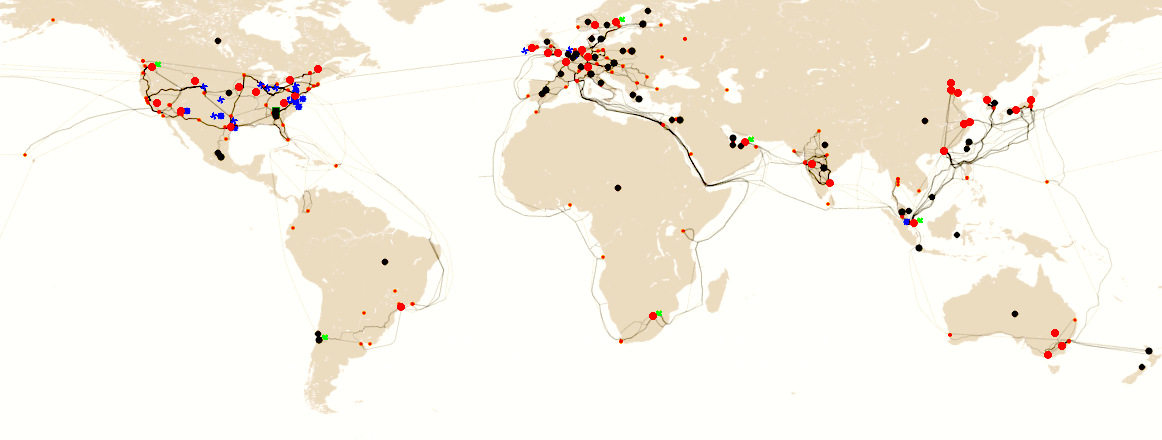
\includegraphics[width=\textwidth]{images/azure_datacenters.png}
    \caption{Azure cloud infrastructure.}
    \end{figure}
\end{column}        
\begin{column}{0.5\textwidth}
    \begin{figure}[!h]
    \centering
    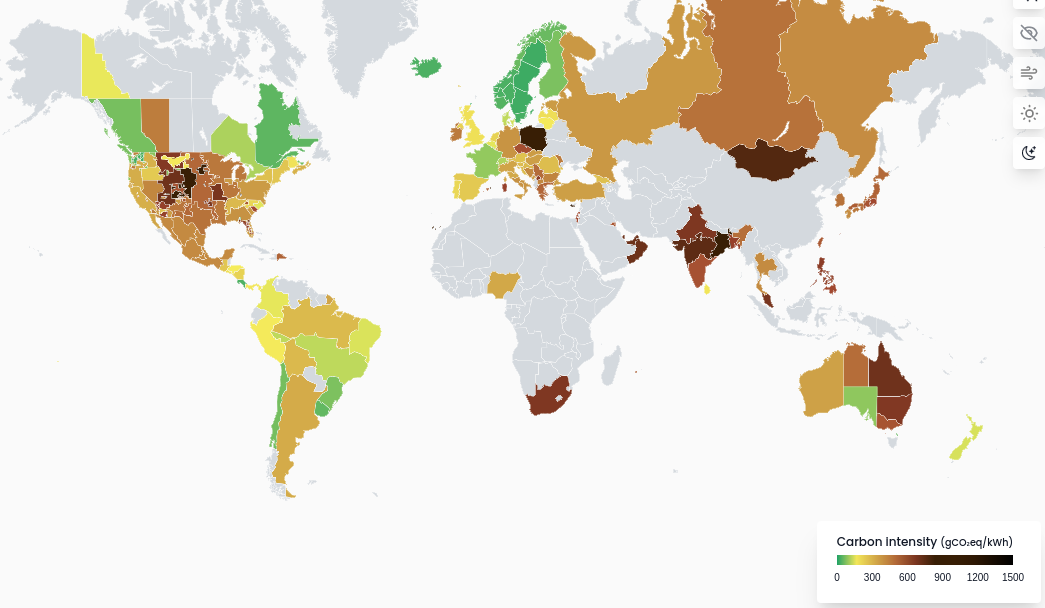
\includegraphics[width=\textwidth]{images/electricity_map.png}
    \caption{ElectricityMap.}
    \end{figure}
    \end{column} 
\end{columns}

  \begin{itemize}
  \item Computing resources on demand for most applications we use
  \item Cloud data centers (DCs) consumes $\approx$1\% of the world's electricity\footcite{IEA_2022} 
  %\item 1\% of the GHG emissions from the electricity sector
  \end{itemize}
\end{frame}


\begin{frame}{Environmental impact of cloud computing}
\begin{columns}        
\begin{column}{0.7\textwidth}
  \begin{itemize}    
  \item Renewable energy in cloud DCs
  \begin{itemize}
    \item Google avg 64\%, up to 97\%\footcite{google_sustainability_report_2023}
 \end{itemize} 
  \item Improvements in efficiency:
  \begin{itemize}
    \item 6 $\times$ workload vs 6\% energy (2010-2018)\footfullcite{masanet2020recalibrating}
  \end{itemize} 
  \item The Green House Gas (GHG) Protocol:
    \begin{enumerate}        
       \item Direct GHG emissions
       \item Electricity indirect GHG emissions
       \item Other indirect GHG emissions: 74\% from Google DCs total carbon footprint
       \end{enumerate}
   \end{itemize}   

\end{column}        
\begin{column}{0.3\textwidth}
      \begin{figure}[!h]
        \centering
        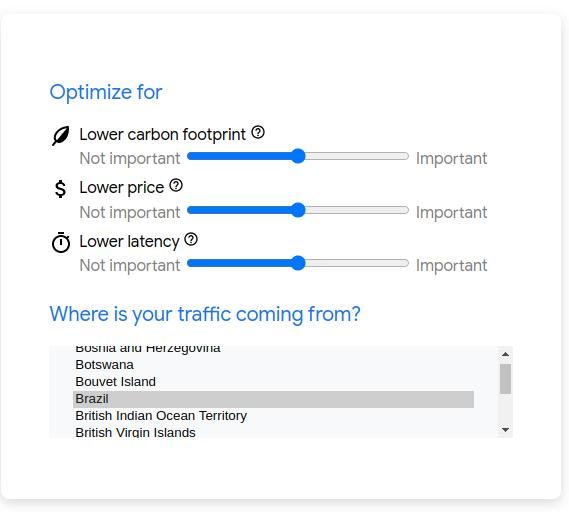
\includegraphics[width=\textwidth]{images/google_region_picker.jpeg}
        \caption{Google's Region picker tool.}
      \end{figure}
    \end{column}        
\end{columns}

\end{frame}


\begin{frame}{Strategies for operating and sizing low-carbon cloud DCs}

\alert{Low-carbon cloud DCs:}

\begin{itemize}
 \item Considering the 3 scopes of the GHG protocol
 \item \ch{CO2}-eq metric
 \begin{itemize}
  \item Compare different GHG gases based in their Global Warming Potential (GWP)
  \item R134a  GWP is 1430:  1g R134a = 1430g \ch{CO2}-eq
\end{itemize}
\end{itemize}

\alert{Carbon-responsive} strategies:\footfullcite{schooler2021carbonaware}  
    \begin{itemize}
        \item  follow-the-renewables
        \item  sizing the renewable and IT infrastructure
     \end{itemize}
     
\end{frame}

\begin{frame}{Strategies for operating and sizing low-carbon cloud DCs}
 
 Main contributions of this thesis:
 
  \begin{itemize}
  
     \item Analysis of the \alert{impact} of adopting the \alert{follow-the-renewables} approaches in both \alert{network congestion} and \alert{energy consumption} 
     \item Modeling for \alert{sizing} the \alert{renewable and IT infrastructure} and \alert{operating} the cloud data centers with \alert{follow-the-renewables} using a Linear Program formulation
     
  \end{itemize}


\end{frame}


\section{Analysis of the impact of follow-the-renewables in network congestion and energy consumption}

\begin{frame}{Follow-the-renewables}

\begin{figure}[h]
\centering
  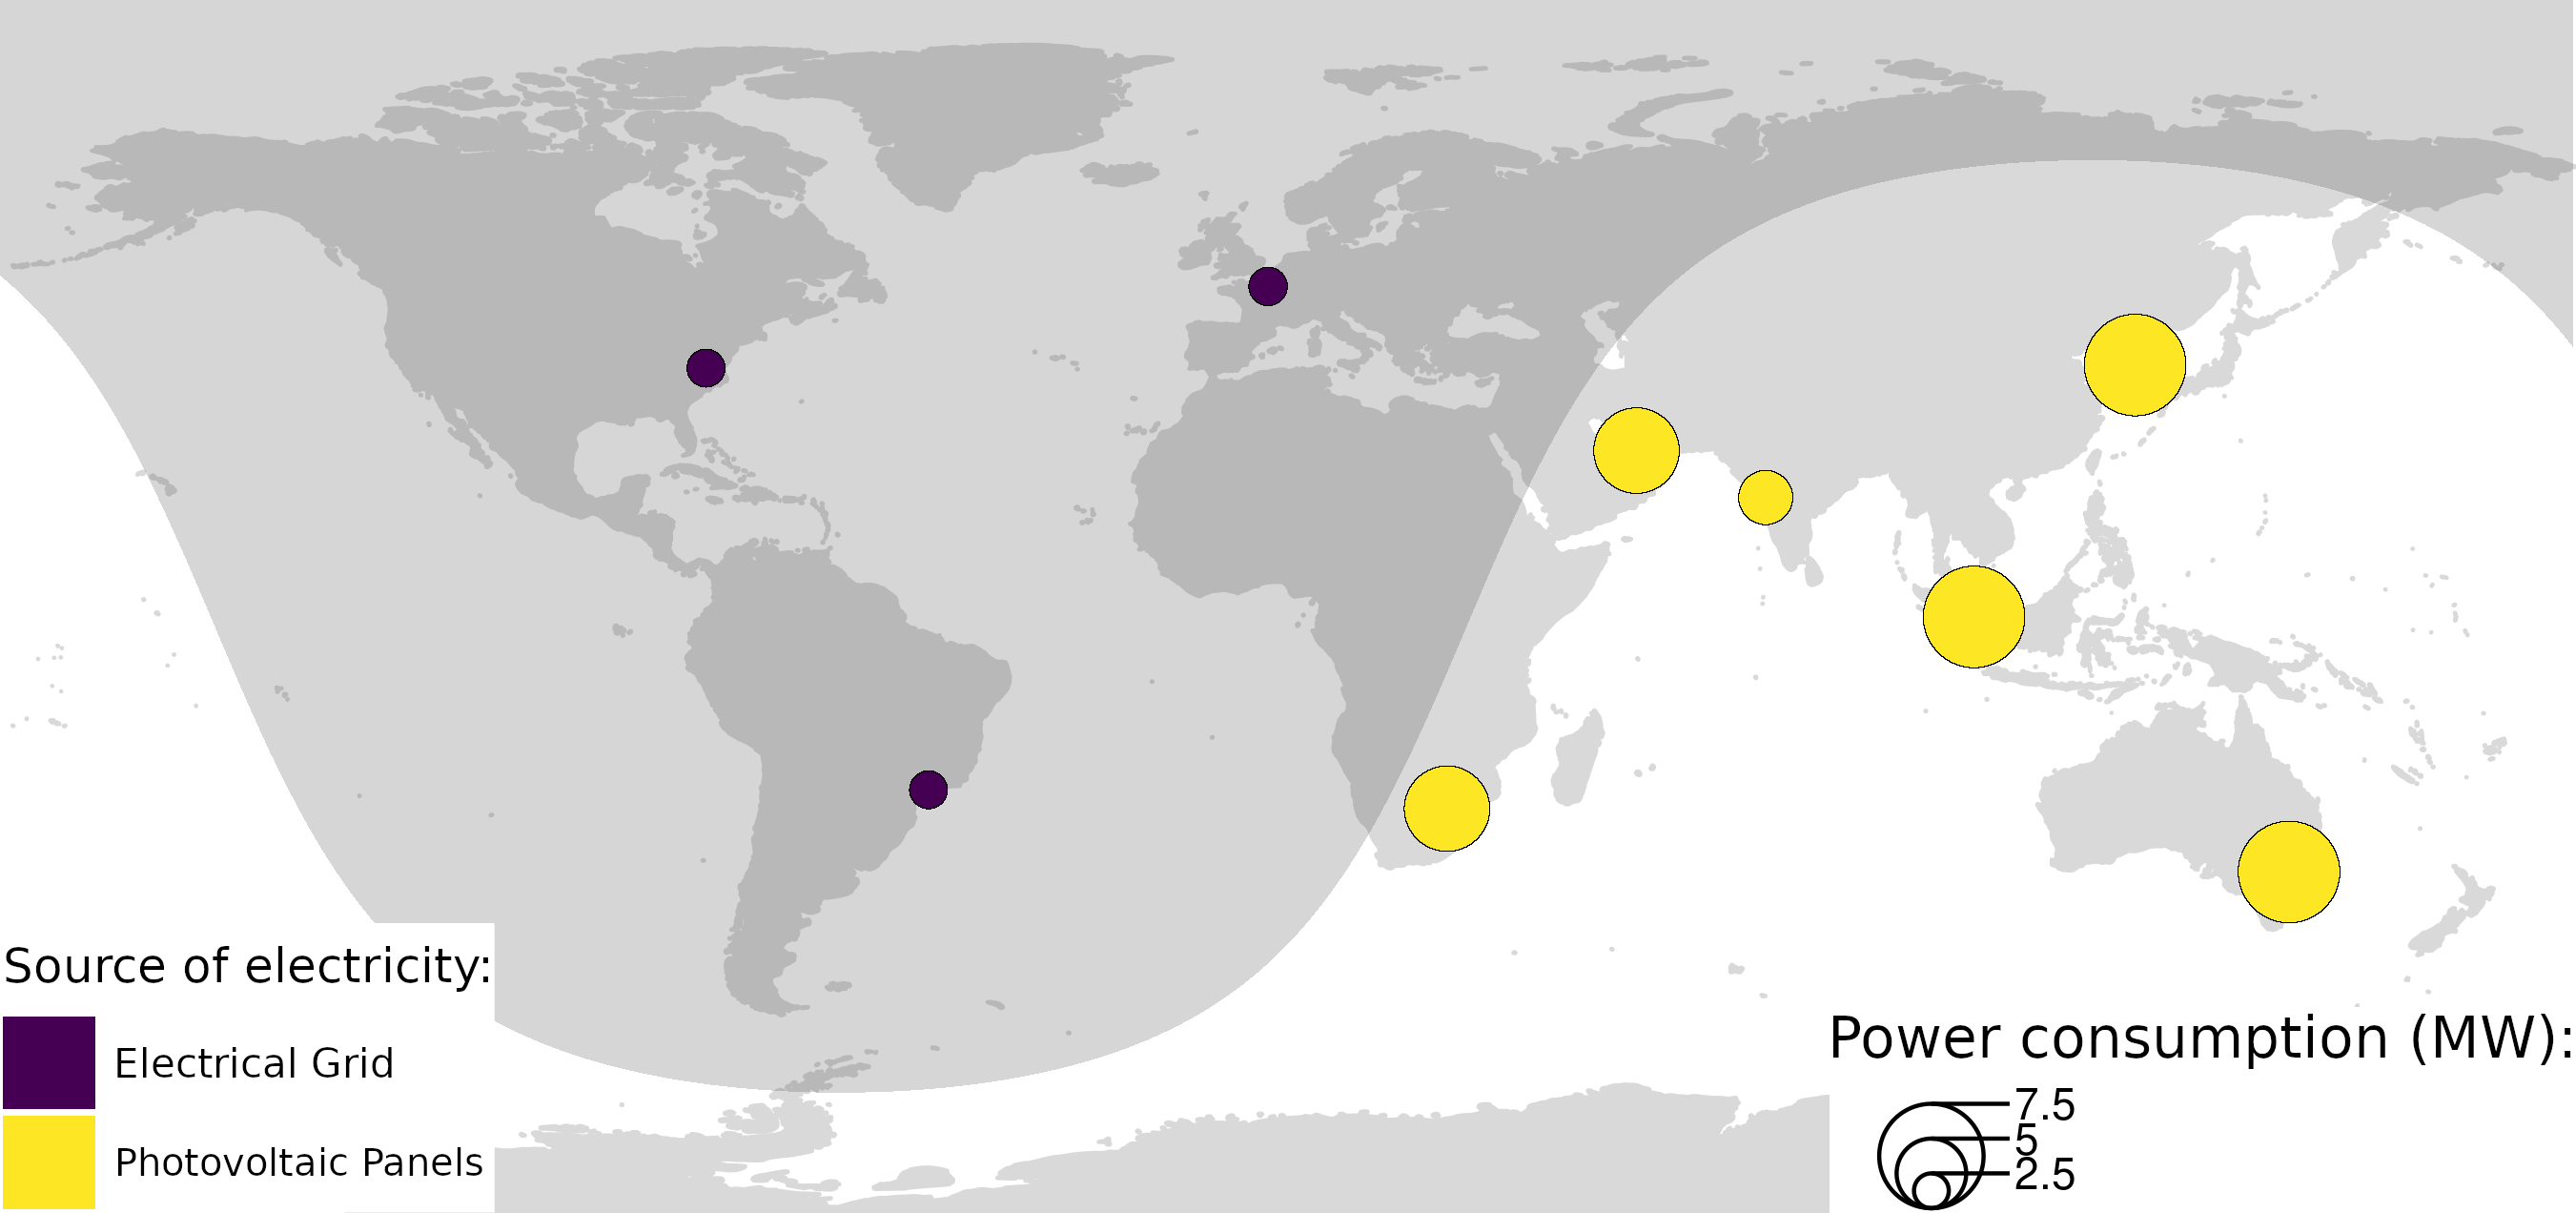
\includegraphics[width=.7\linewidth]{images/example_follow_the_renewables.png}
  \caption{An example of a cloud federation that adopts the follow-the-renewables strategy.}
  \label{fig:ex_follow_the_renewables}
\end{figure}
\vspace{-10pt}

\begin{itemize}    
  \item Allocates/Migrates the workload to the data centers (DCs) that have more renewable (green) power available
 \item Extra computations proportional to the migration duration 
 \item What is the impact in \alert{network congestion} and \alert{energy consumption}? 
  \end{itemize}
\end{frame}


%\begin{frame}{Methodology}

  %\begin{itemize}

  %\item Extension of the NEMESIS framework:
  %\begin{itemize}
   %   \item Consider network topology
    %  \item Usage of the network links while migrating
  %\end{itemize}
    
 %\item Experimental validation:
  %\begin{itemize}
   %   \item Baselines from literature (WSNB, FollowME@S)
    %  \item Cloud platform, workload,  and renewable traces inspired in real-world values
     % \item metrics: brown energy consumption, time spent migrating the workload
  % \end{itemize}
  
% \end{itemize}  
% \end{frame}


\begin{frame}{Different usages of the follow-the-renewables}
\newcommand{\tikzxmark}{%
\tikz[scale=0.25] {
    \draw[line width=1,line cap=round] (0,0) to [bend left=6] (1,1);
    \draw[line width=1,line cap=round] (0.2,0.95) to [bend right=3] (0.8,0.05);
}}
\newcommand{\tikzcmark}{%
\tikz[scale=0.25] {
    \draw[line width=1,line cap=round] (0.25,0) to [bend left=10] (1,1);
    \draw[line width=1,line cap=round] (0,0.35) to [bend right=1] (0.23,0);
}}




    



 
 \begin{table}[!h]
    \caption{Comparison between different approaches to adopt follow-the-renewables.}\label{tab:total_energy_cons} \centering
    \begin{tabular}{|l|c|c|c|}      
      \hline
      \textbf{Algorithm} & \textbf{Allocation} &  \textbf{Migration} & \textbf{Network} \\
      \hline
      NEMESIS\footfullcite{NEMESIS}  & \tikzcmark & \tikzcmark & \tikzcmark \\
      \hline
      FollowMe@S Intra \footfullcite{ALI2021110907} & \tikzcmark & \tikzcmark  &     \tikzxmark\\
      \hline
      FollowMe@S Inter & \tikzcmark & \tikzcmark &     \tikzxmark \\
      \hline
      WSNB\footfullcite{XU2020191} & \tikzcmark &     \tikzxmark &     \tikzxmark
      \\
      \hline
    \end{tabular}
  \end{table}
\end{frame}

\begin{frame}{Computational simulations}
  \begin{itemize}        
  \item Simgrid: framework to simulate large scale distributed systems
    \begin{itemize}        
  %  \item Well-validated by the scientific community (over 20 years of
   %   usage)
    \item Servers' power consumption: linear model based on CPU usage
     \item Flow-level TCP modeling of the network
     \end{itemize}
   \item Model of live-migration's power consumption:
    \begin{itemize}        
    \item one CPU core is used in the target host during the migration
   \end{itemize}
  \end{itemize}
\end{frame}

\begin{frame}{Input: cloud infrastructure} 
  \begin{columns}    
    \begin{column}{0.5\textwidth}
      \begin{itemize}        
      \item Based on a real example: Grid'5000
      \item 1035 homogeneous servers distributed among 9 DCs
        \begin{itemize}        
        \item 2 x Intel Xeon E5-2630 (6 CPU cores per processor)
        \item 32 GB RAM
        \end{itemize}
      \item Network:
        \begin{itemize}                         
        \item 1Gbps links intra DC
        \item 10Gbps links inter DC
        \end{itemize}
      \end{itemize}
    \end{column}
    
    \begin{column}{0.5\textwidth}
      \begin{figure}[!h]
        \centering
        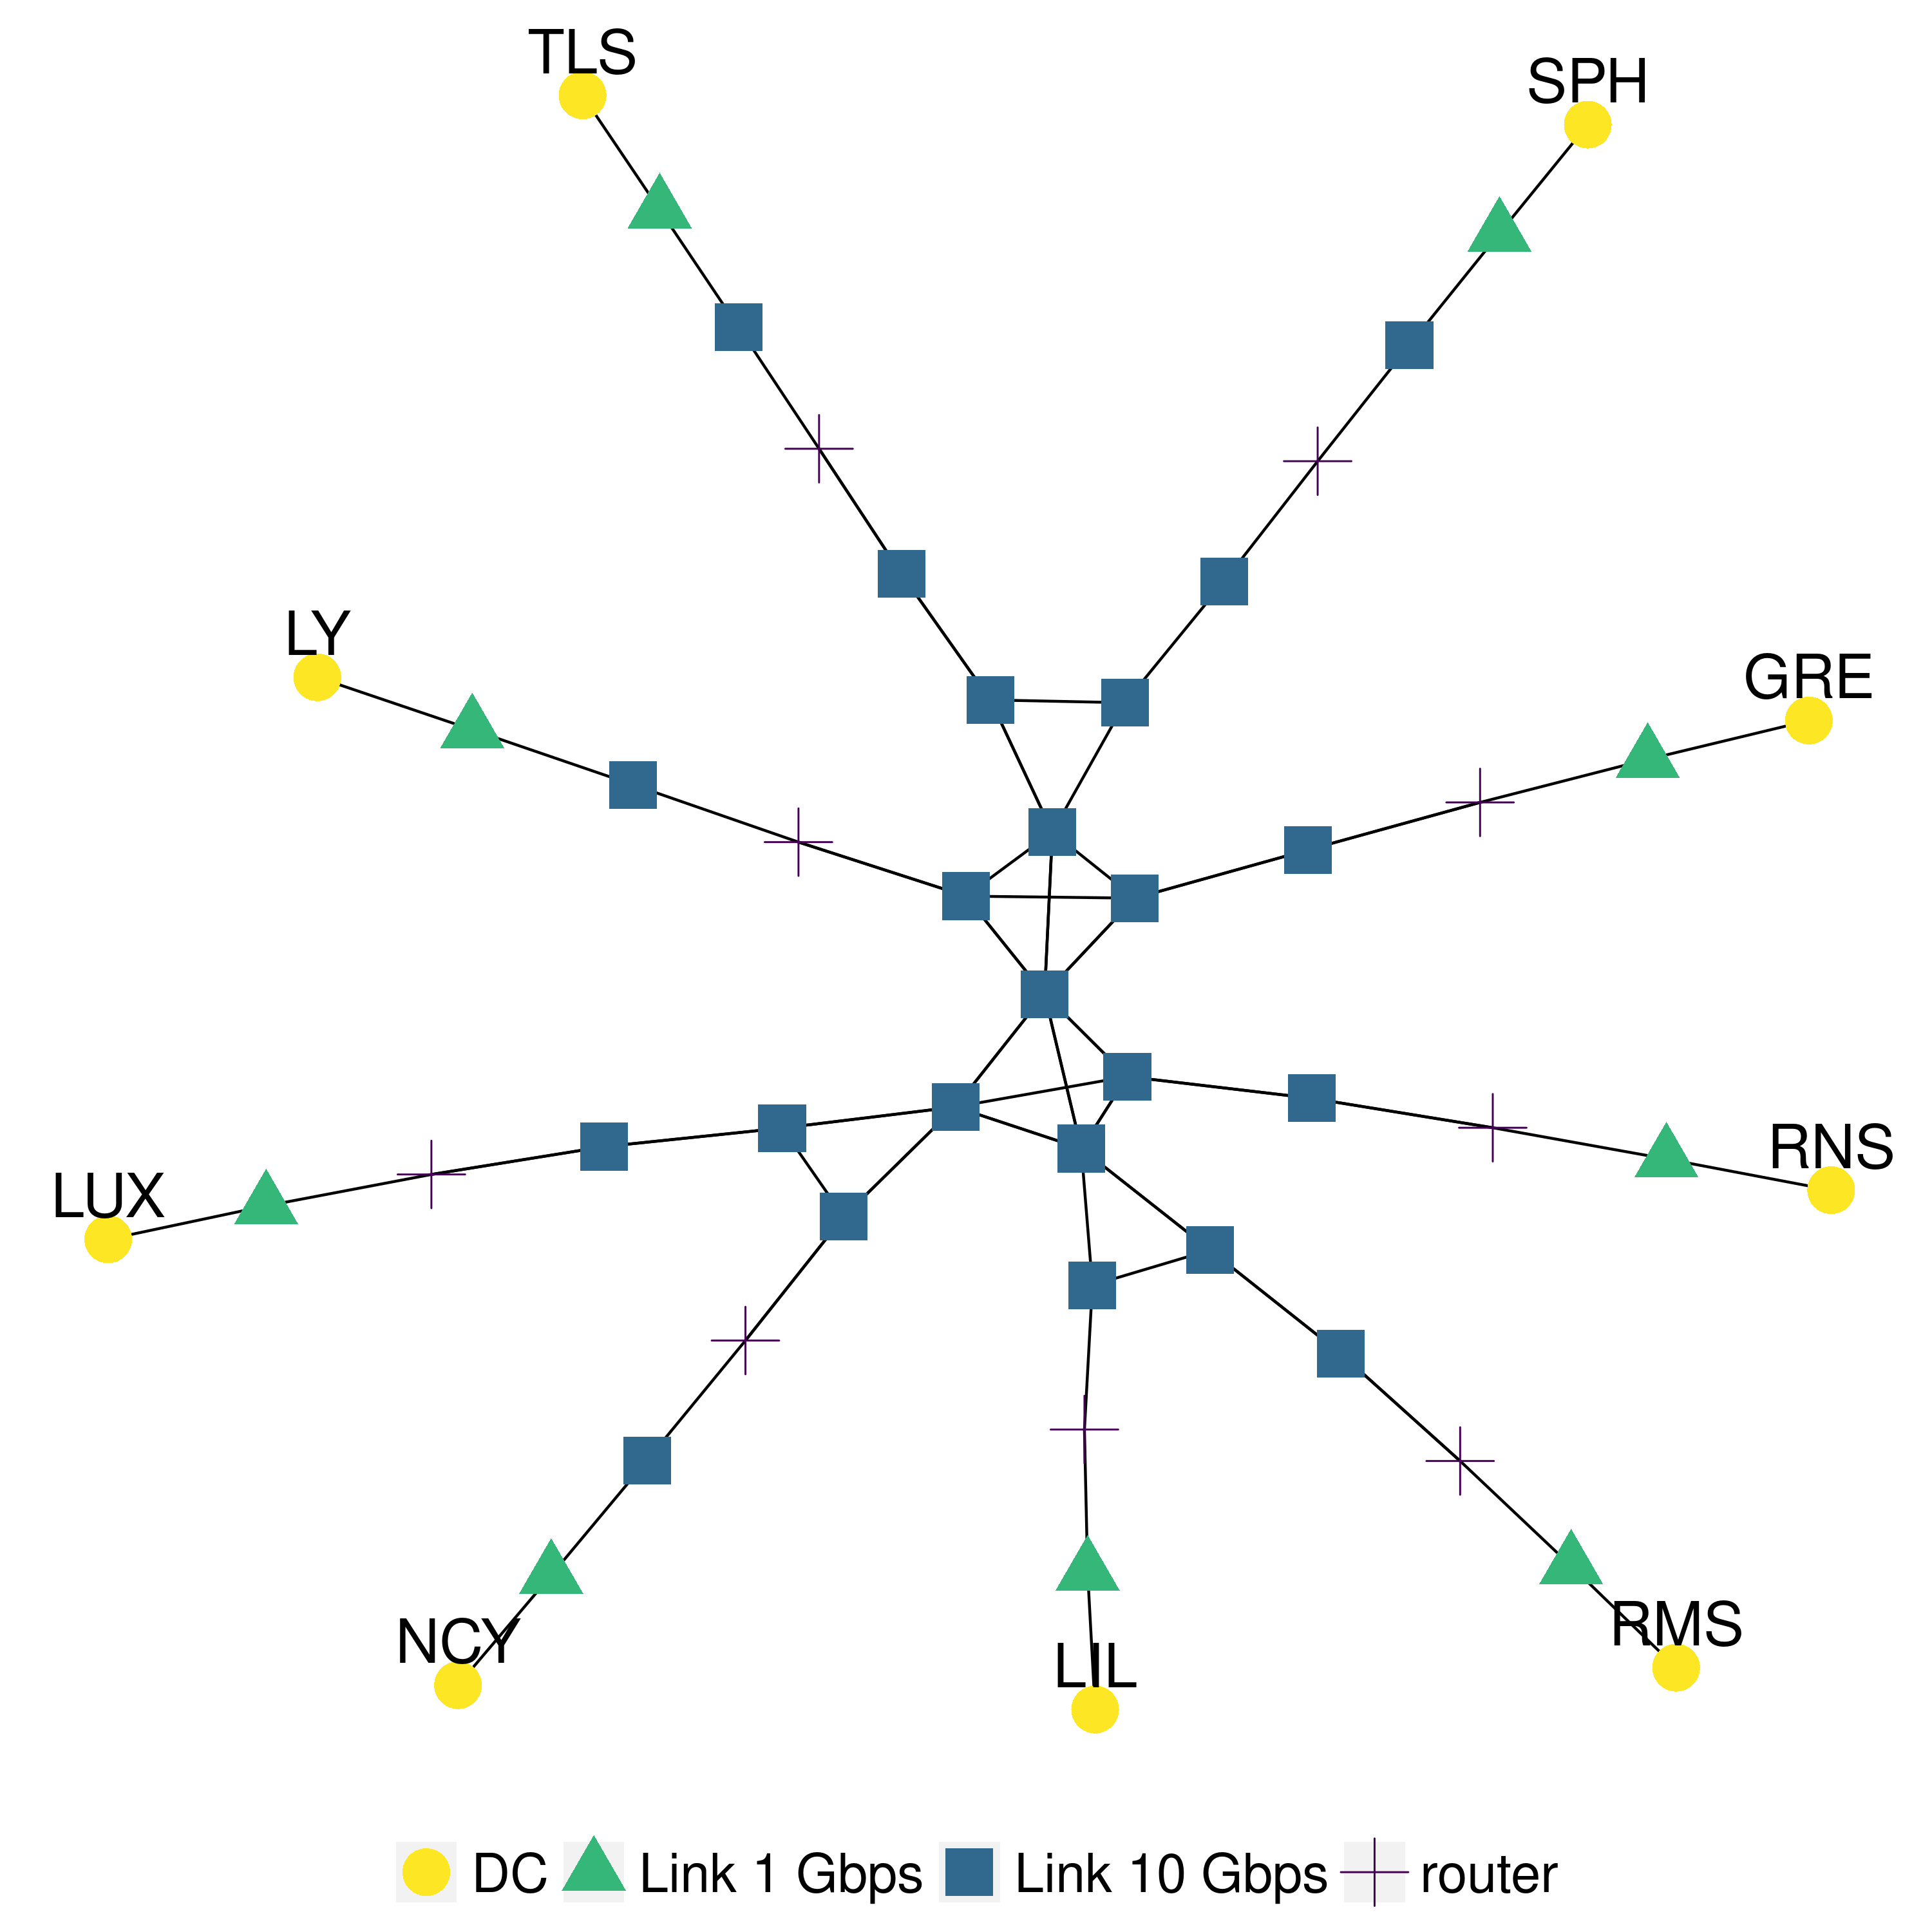
\includegraphics[width=.9\textwidth]{images/topology.png}
        \caption{How the DCs are interconnected in the network.}
      \end{figure}
    \end{column}        
  \end{columns}    
\end{frame}


\begin{frame}{Input: green energy traces}  
  \begin{figure}[!h]
    \centering
    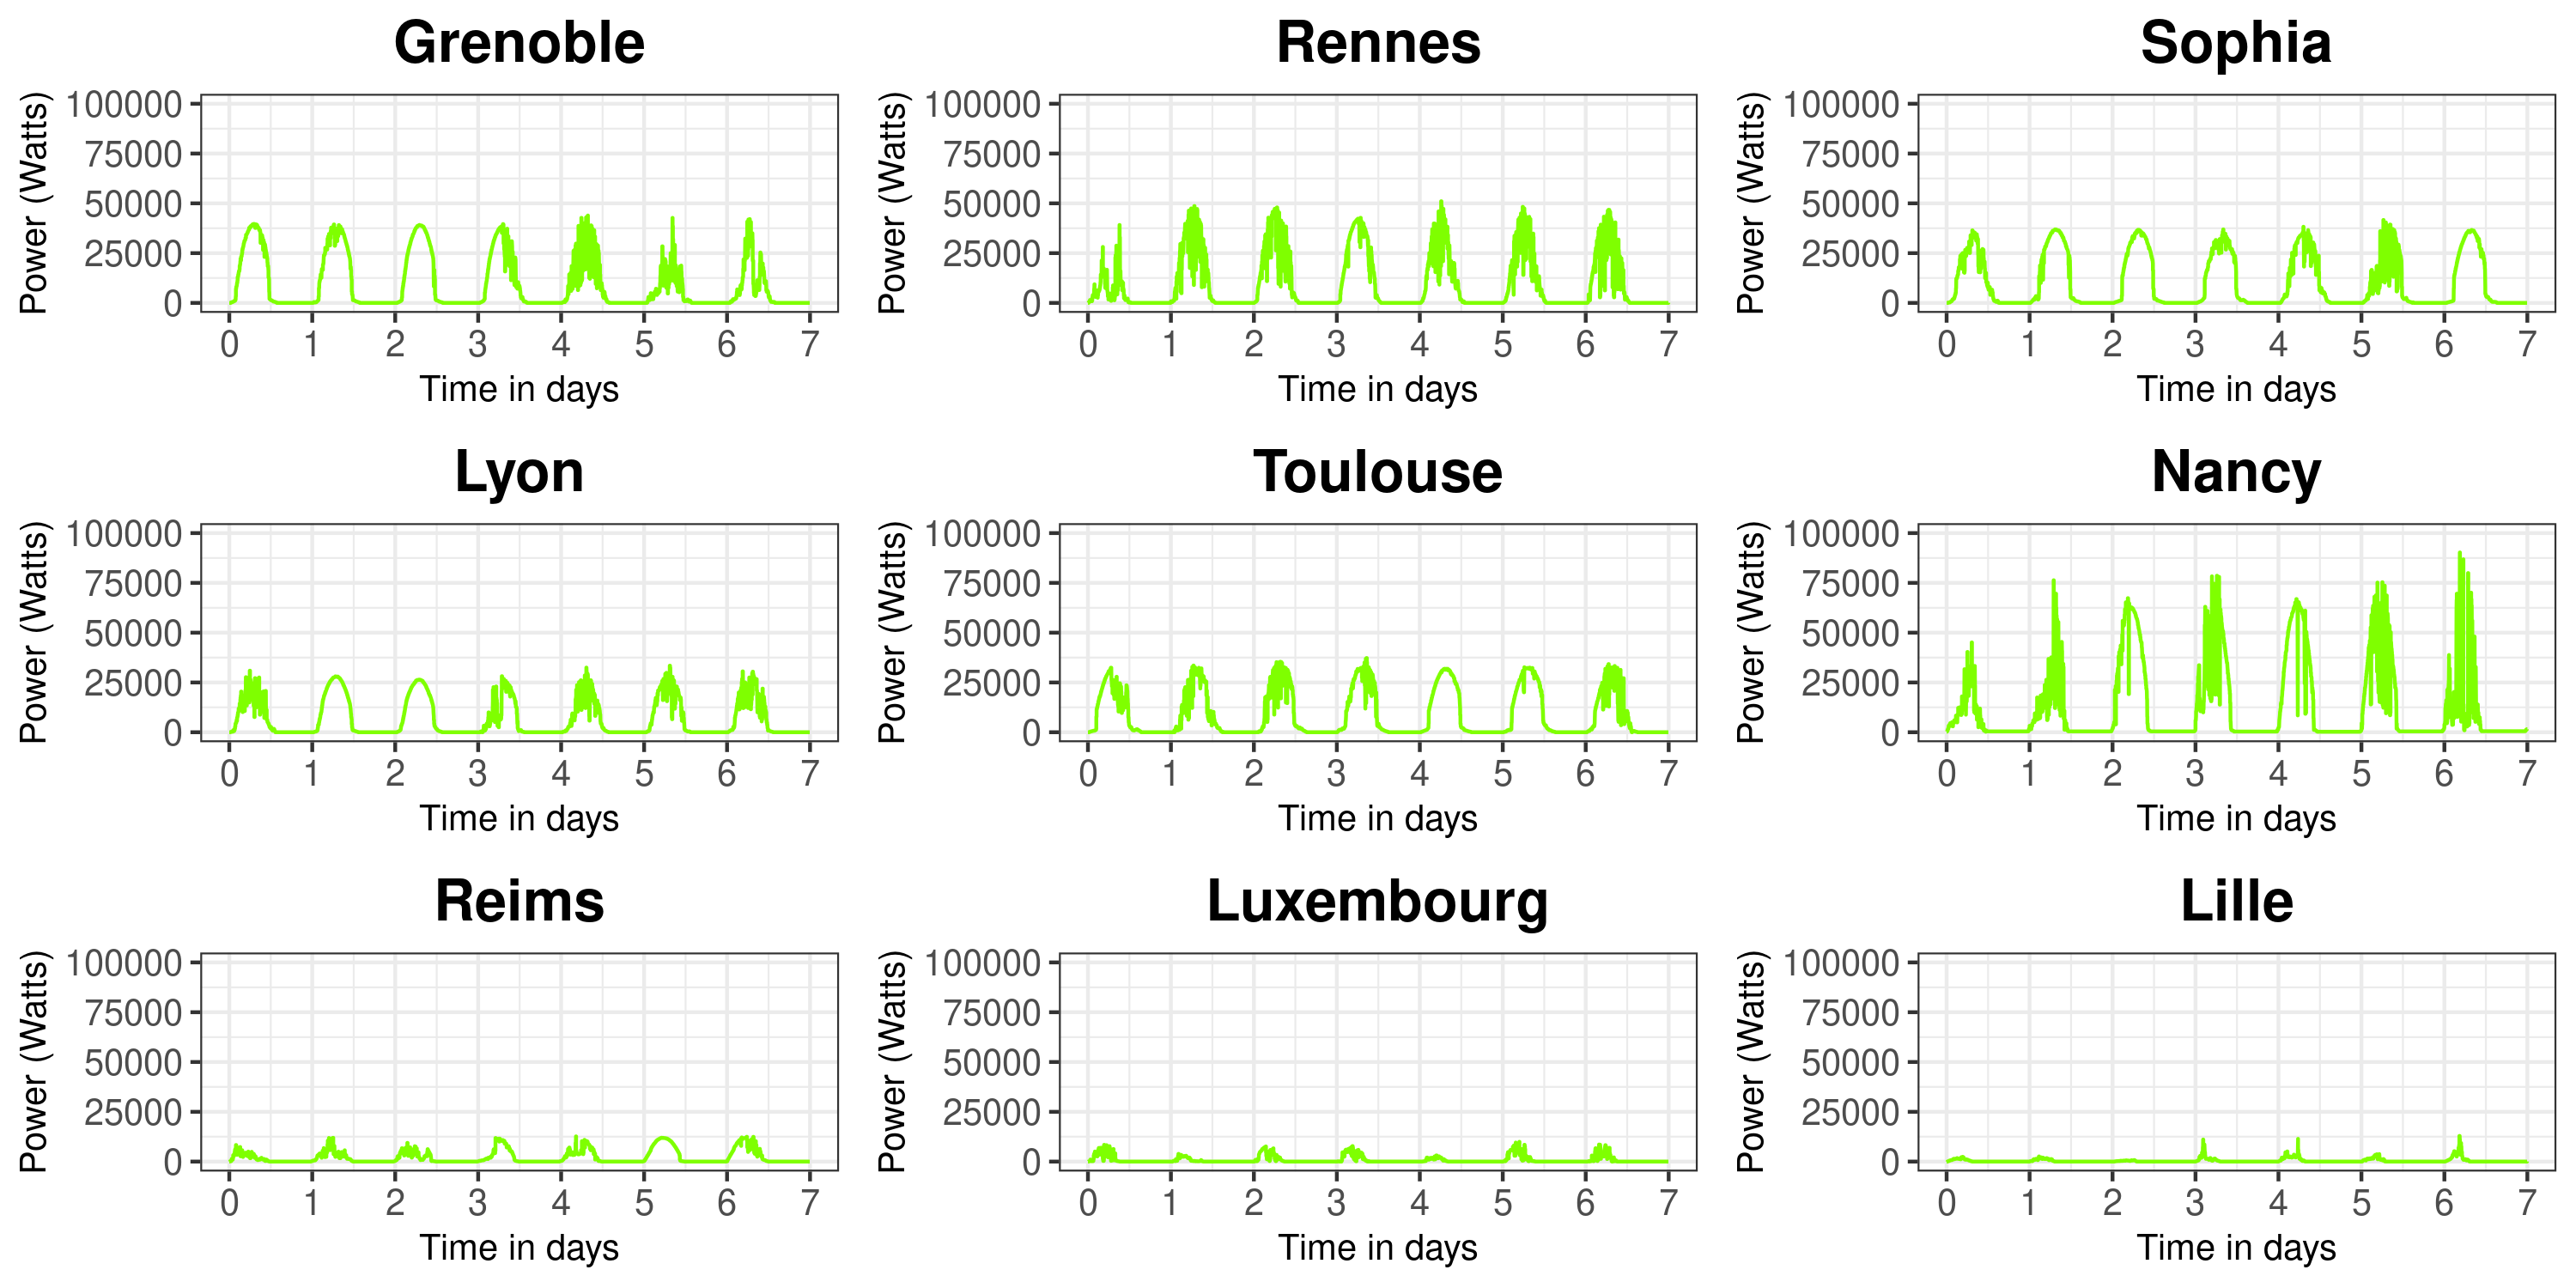
\includegraphics[width=\textwidth]{images/green_pow_production.png}
    \caption{Green energy power production per DC - Source of data:
      Photovolta project.}
  \end{figure}
\end{frame}

\begin{frame}{Input: workloads}

  \begin{columns}
    
    \begin{column}{0.5\textwidth}          
      \begin{itemize}
      \item Virtual machines
      \item Traces samples from real cloud providers:
        \begin{itemize}        
        \item Google (2011): 380k VMs
        \item Azure (2020):  300k VMs
        \end{itemize}
      \item Information extracted:
        \begin{itemize}        
        \item Submission time, CPU cores requested, runtime            
        \end{itemize}              

      \item RAM = 2GB per CPU cores (t2.small)
        \item No network usage
      \end{itemize}
    \end{column}
    
    \begin{column}{0.5\textwidth}
      \begin{figure}[!h]
        \centering
        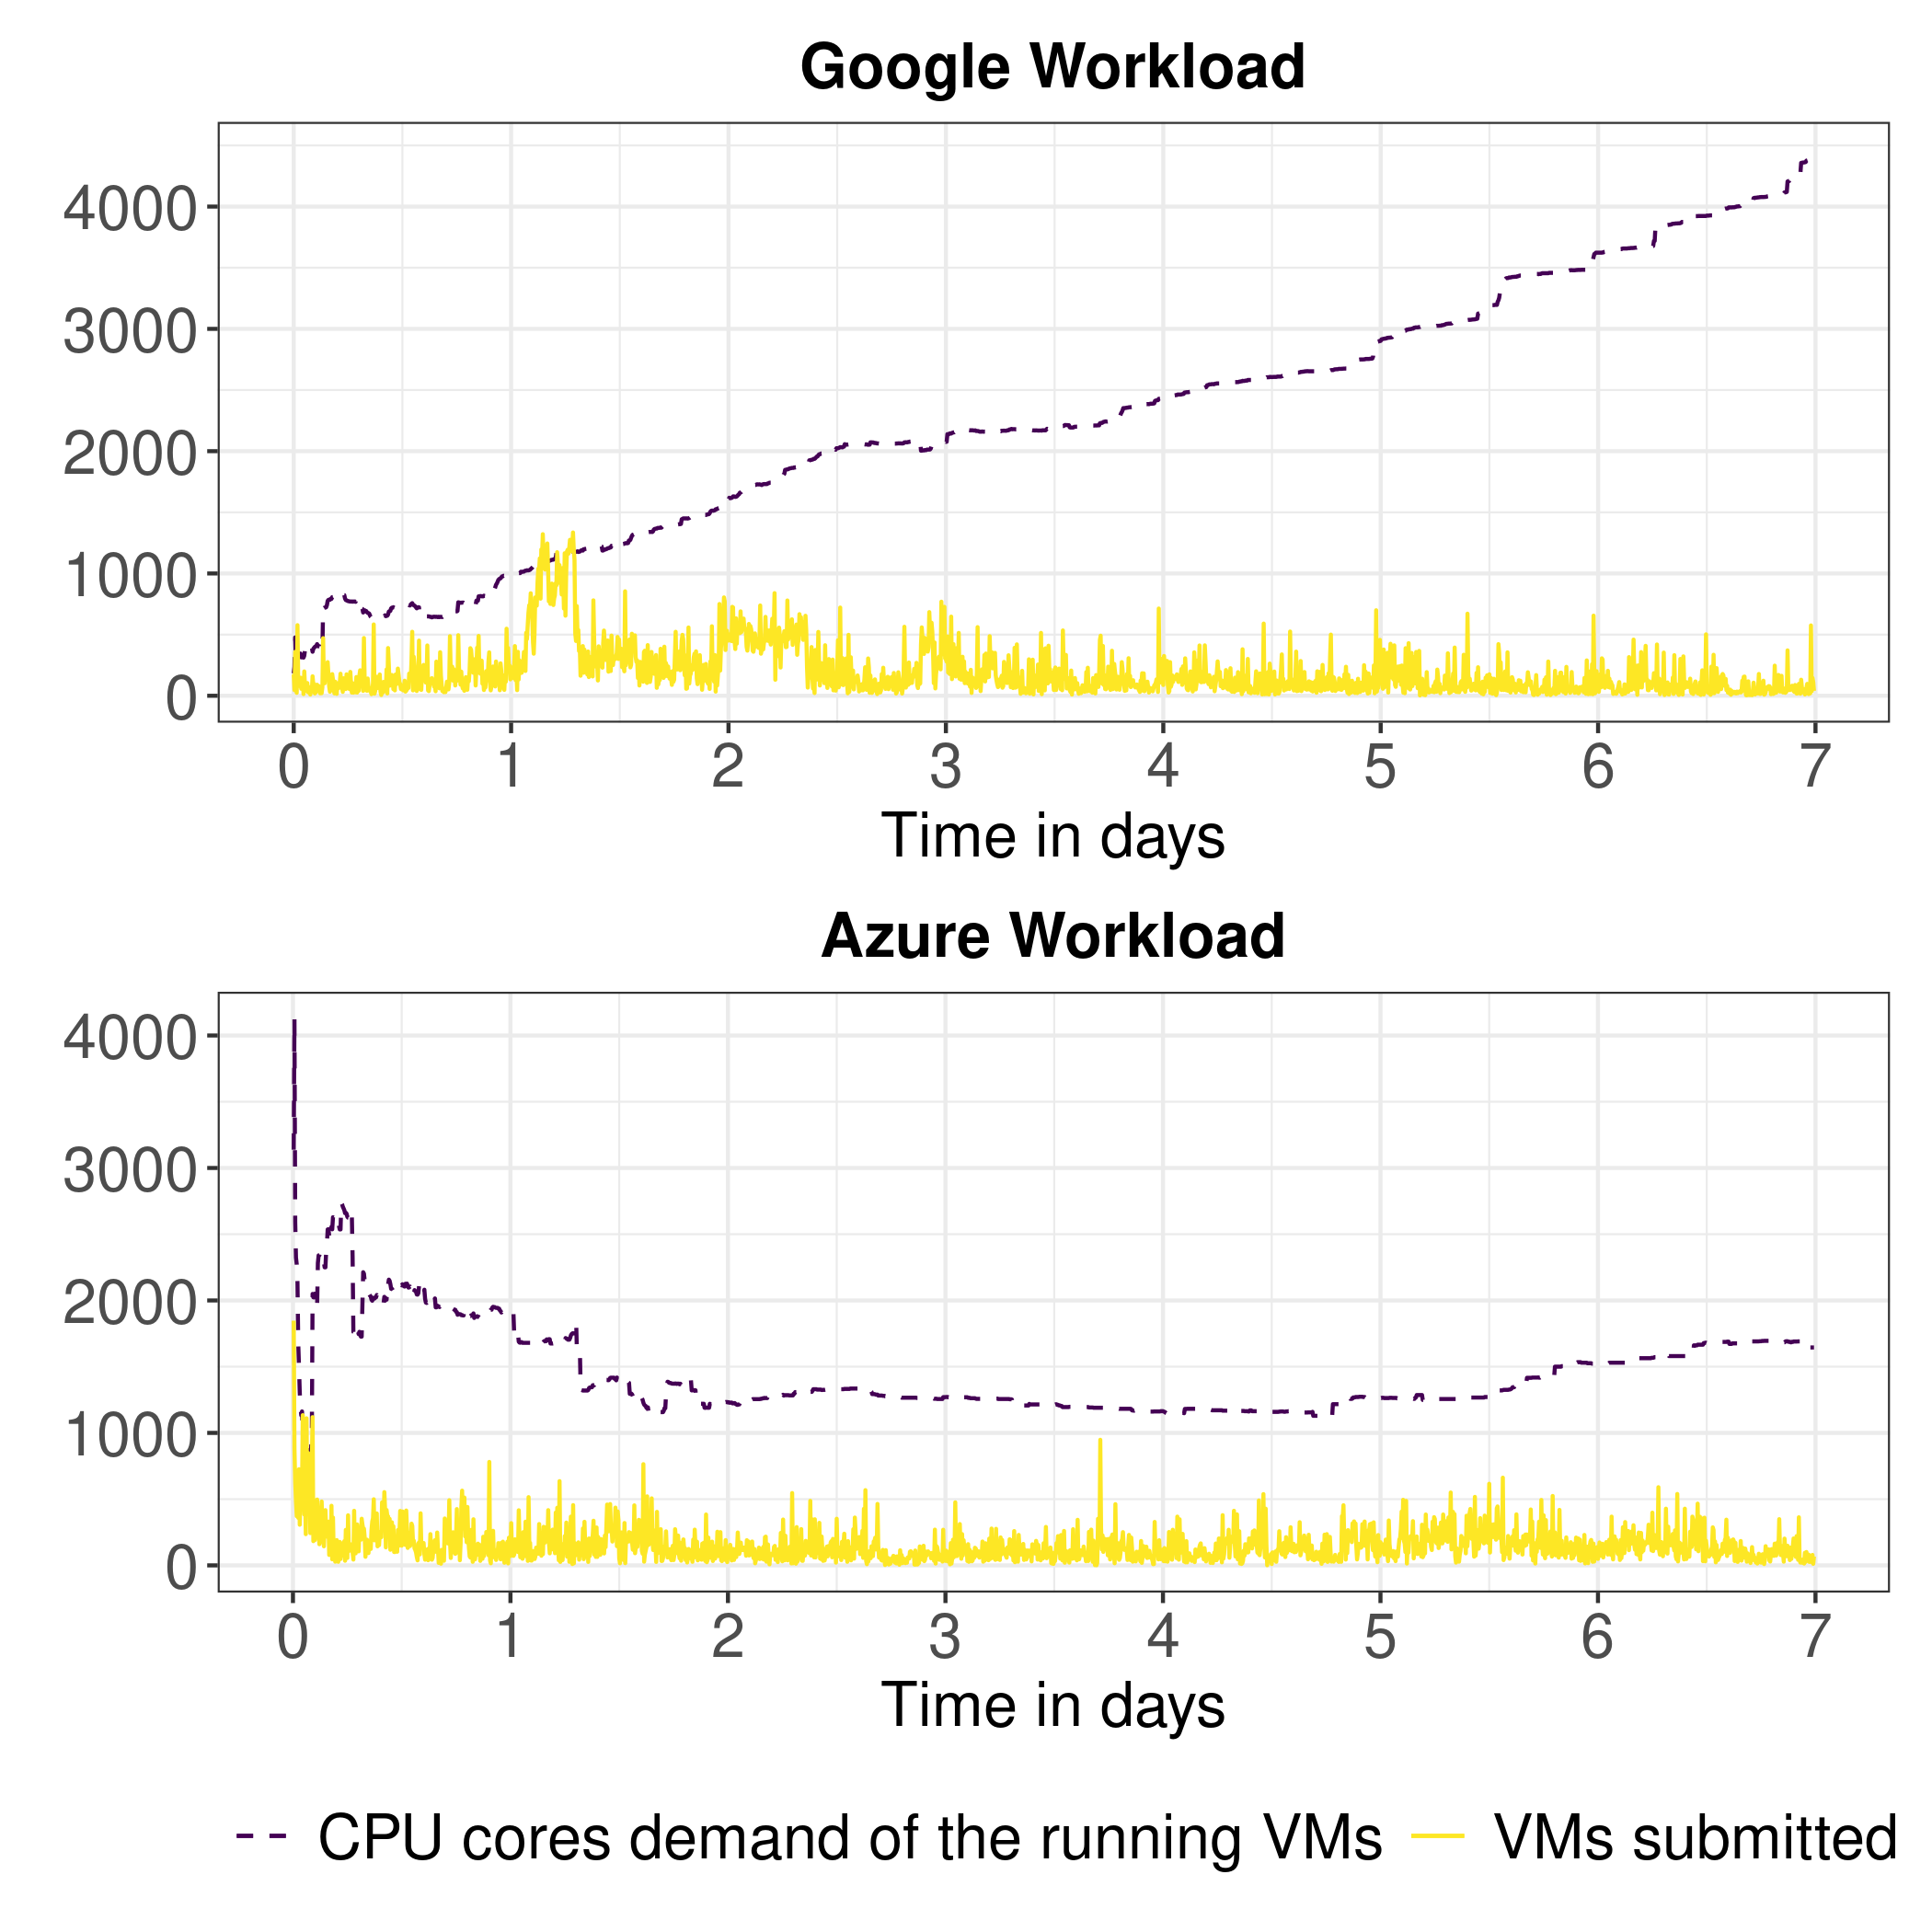
\includegraphics[width=\textwidth]{images/workloads.png}
        \caption{Workloads used for the simulations.}
      \end{figure}
    \end{column}    
  \end{columns}    
  
\end{frame}

\begin{frame}{Total and brown energy consumption}  
  \begin{table}[!h]
    \caption{Comparison of energy consumption (MWh) for the Azure workload.}\label{tab:total_energy_cons} \centering
    \begin{tabular}{|l|r|r|}      
      \hline
      \textbf{Algorithm} & \textbf{Total} &  \textbf{Non-renewable} \\
      \hline
      NEMESIS  & 30.43 & 21.21 \\
 %    \hline
 %     c-NEMESIS & 30.55 & 21.20 \\
      \hline
      FollowMe@S Inter & 31.69 & 22.40 \\
      \hline
      FollowMe@S Intra & 31.69 & 22.41 \\      
      \hline
      WSNB & 33.56 & 24.23 \\
      \hline
    \end{tabular}
  \end{table}  
  \pause

\begin{itemize}
    \item Impact of \textbf{network congestion} in the \textbf{energy consumption}?
    \item Using network information to plan the migrations without congestion
\end{itemize}
\end{frame}

\begin{frame}{NEMESIS}
  \textbf {``\alert{N}etwork-aware \alert{E}nergy-efficient
    \alert{M}anagement framework for distribut\alert{E}d
    cloud\alert{S} \alert{I}nfrastructures with on-\alert{S}ite
    photovoltaic production''}\footfullcite{NEMESIS}  
  \begin{columns}        
    \begin{column}{0.4\textwidth}
Main steps:
\small
\begin{itemize}
    \item Pre-allocation of incoming Virtual Machines (VMs)
    \item Revision of pre-allocations
    \item Migration of the running VMs
    \item Servers consolidation
\end{itemize}
\end{column}   

\begin{column}{0.6\textwidth}
      \begin{figure}[!h]
        \centering
        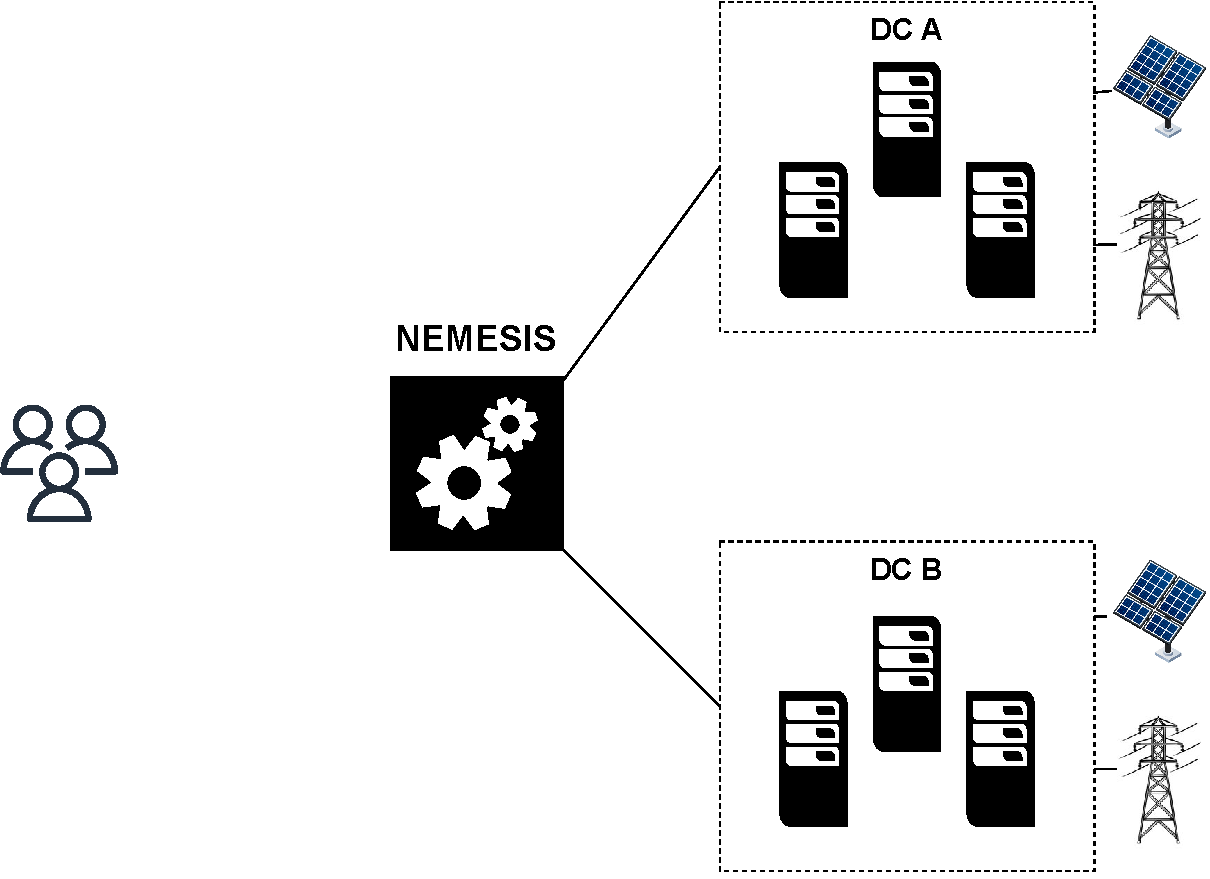
\includegraphics[width=.85\textwidth]{images/nemesis.pdf}
        \caption{NEMESIS framework.}
      \end{figure}
    \end{column}        

\end{columns}
\end{frame}
\addtocounter{framenumber}{-1}


\begin{frame}{NEMESIS}
  \textbf {``\alert{N}etwork-aware \alert{E}nergy-efficient
    \alert{M}anagement framework for distribut\alert{E}d
    cloud\alert{S} \alert{I}nfrastructures with on-\alert{S}ite
    photovoltaic production''}\footfullcite{NEMESIS}  
  \begin{columns}        
    \begin{column}{0.4\textwidth}
Main steps:
\small
\begin{itemize}
    \item \alert{\textbf{Pre-allocation of incoming Virtual Machines (VMs)}}
    \item Revision of pre-allocations
    \item Migration of the running VMs
    \item Servers consolidation
\end{itemize}
\end{column}   

\begin{column}{0.6\textwidth}
      \begin{figure}[!h]
        \centering
        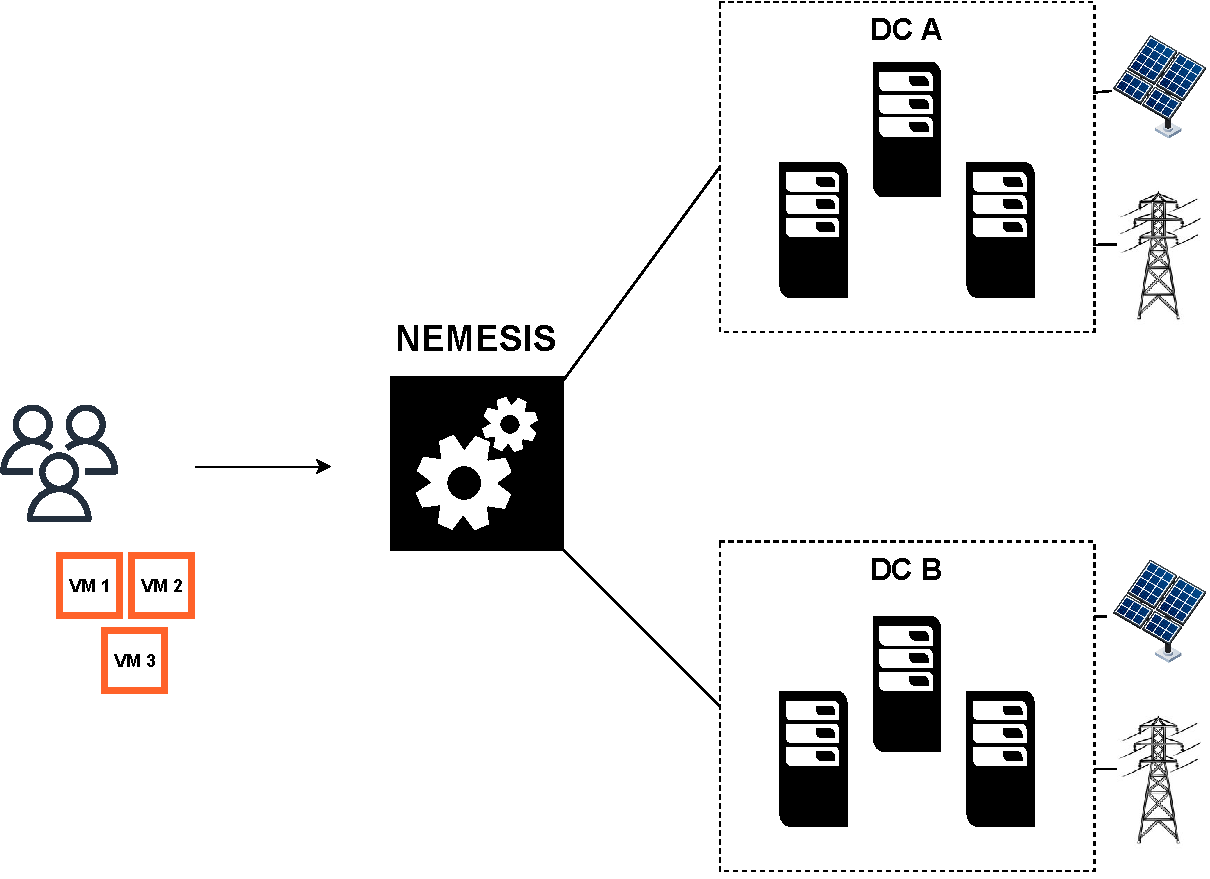
\includegraphics[width=.85\textwidth]{images/nemesis_pre_aloc_1.pdf}
        \caption{NEMESIS framework.}
      \end{figure}
    \end{column}        

\end{columns}
\end{frame}


\addtocounter{framenumber}{-1}


\begin{frame}{NEMESIS}
  \textbf {``\alert{N}etwork-aware \alert{E}nergy-efficient
    \alert{M}anagement framework for distribut\alert{E}d
    cloud\alert{S} \alert{I}nfrastructures with on-\alert{S}ite
    photovoltaic production''}\footfullcite{NEMESIS}  
  \begin{columns}        
    \begin{column}{0.4\textwidth}
Main steps:
\small
\begin{itemize}
    \item \alert{\textbf{Pre-allocation of incoming Virtual Machines (VMs)}}
    \item Revision of pre-allocations
    \item Migration of the running VMs
    \item Servers consolidation
\end{itemize}
\end{column}   

\begin{column}{0.6\textwidth}
      \begin{figure}[!h]
        \centering
        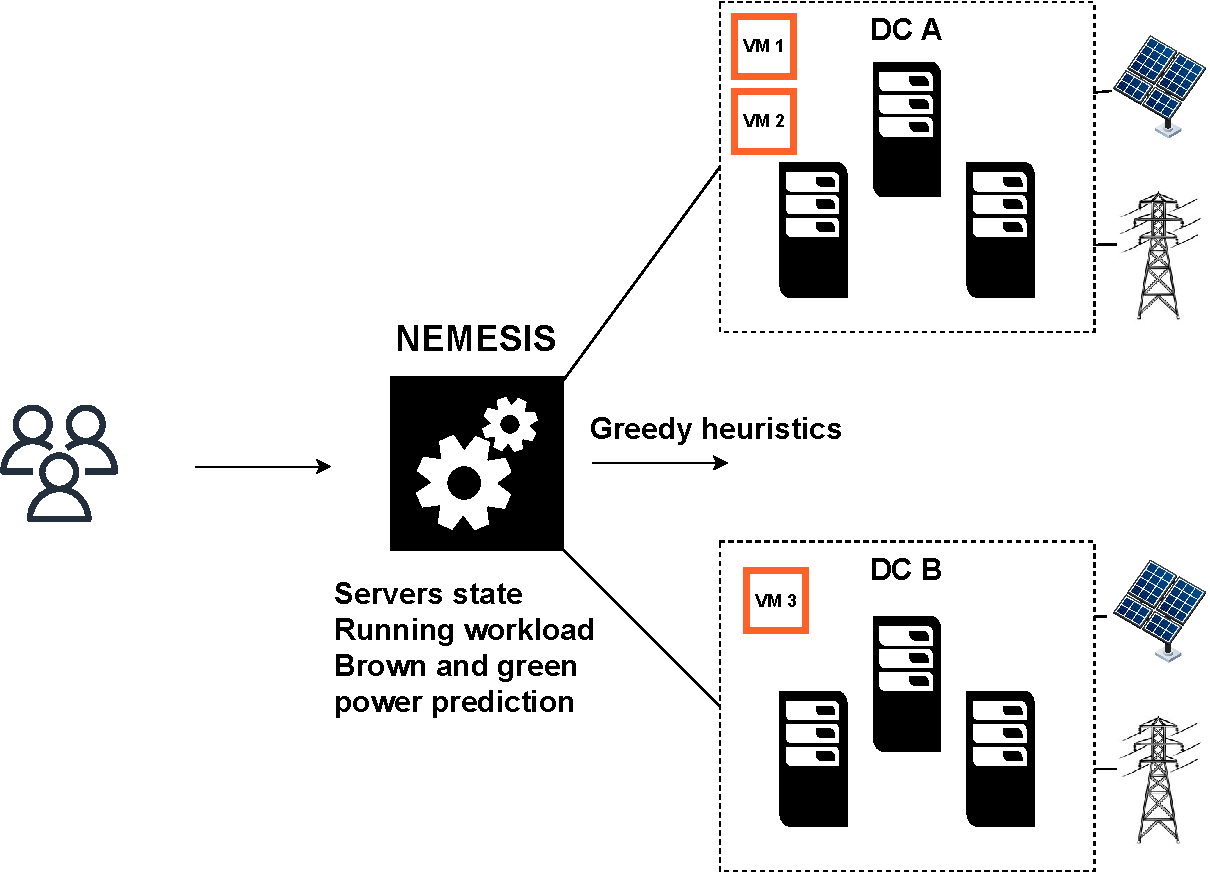
\includegraphics[width=.85\textwidth]{images/nemesis_pre_aloc_2.pdf}
        \caption{NEMESIS framework.}
      \end{figure}
    \end{column}        

\end{columns}
\end{frame}




\begin{frame}{NEMESIS}
  \textbf {``\alert{N}etwork-aware \alert{E}nergy-efficient
    \alert{M}anagement framework for distribut\alert{E}d
    cloud\alert{S} \alert{I}nfrastructures with on-\alert{S}ite
    photovoltaic production''}\footfullcite{NEMESIS}  
  \begin{columns}        
    \begin{column}{0.4\textwidth}
Main steps:
\small
\begin{itemize}
    \item Pre-allocation of incoming Virtual Machines (VMs)
    \item \alert{\textbf{Revision of pre-allocations}}
    \item Migration of the running VMs
    \item Servers consolidation
\end{itemize}
\end{column}   

\begin{column}{0.6\textwidth}
      \begin{figure}[!h]
        \centering
        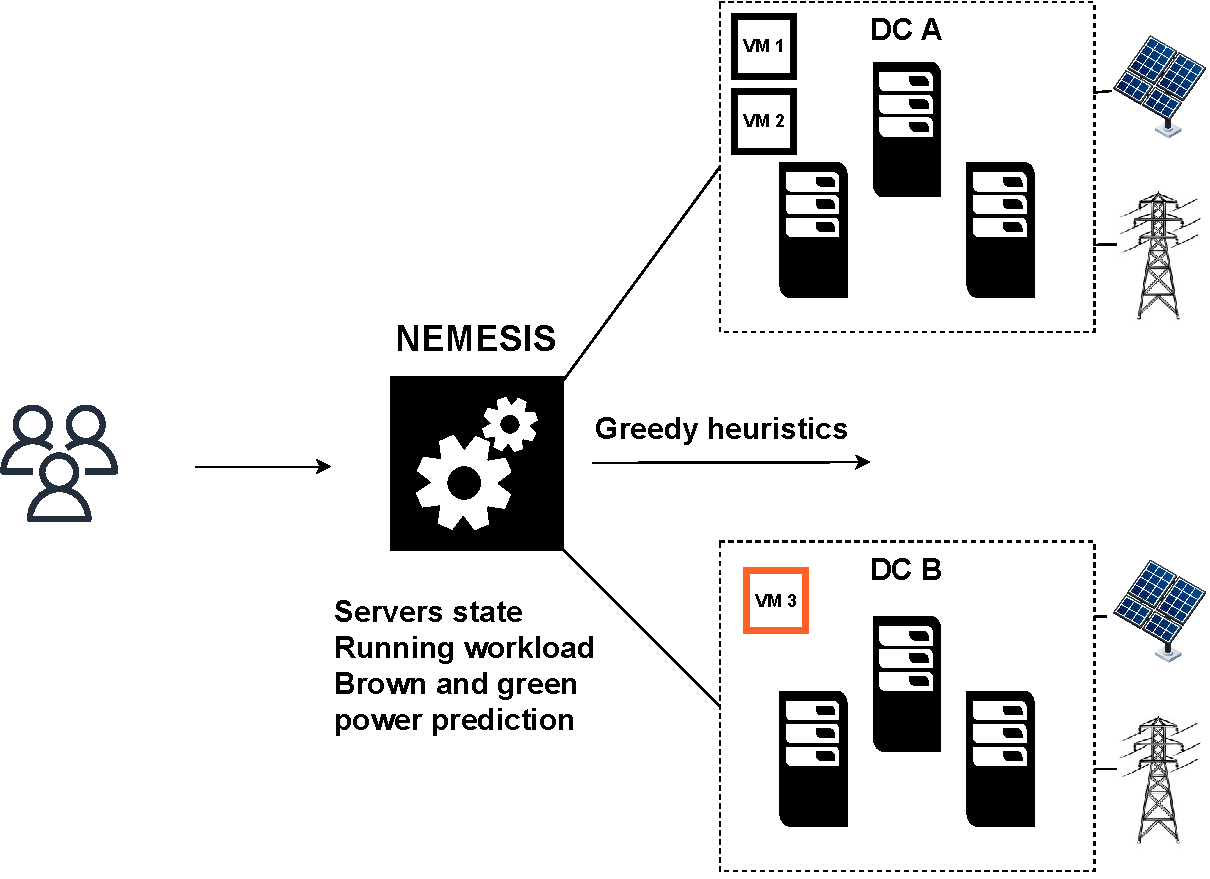
\includegraphics[width=.85\textwidth]{images/nemesis_review_1.pdf}
        \caption{NEMESIS framework.}
      \end{figure}
    \end{column}        

\end{columns}
\end{frame}

\addtocounter{framenumber}{-1}


    

\begin{frame}{NEMESIS}
  \textbf {``\alert{N}etwork-aware \alert{E}nergy-efficient
    \alert{M}anagement framework for distribut\alert{E}d
    cloud\alert{S} \alert{I}nfrastructures with on-\alert{S}ite
    photovoltaic production''}\footfullcite{NEMESIS}  
  \begin{columns}        
    \begin{column}{0.4\textwidth}
Main steps:
\small
\begin{itemize}
    \item Pre-allocation of incoming Virtual Machines (VMs)
    \item \alert{\textbf{Revision of pre-allocations}}
    \item Migration of the running VMs
    \item Servers consolidation
\end{itemize}
\end{column}   

\begin{column}{0.6\textwidth}
      \begin{figure}[!h]
        \centering
        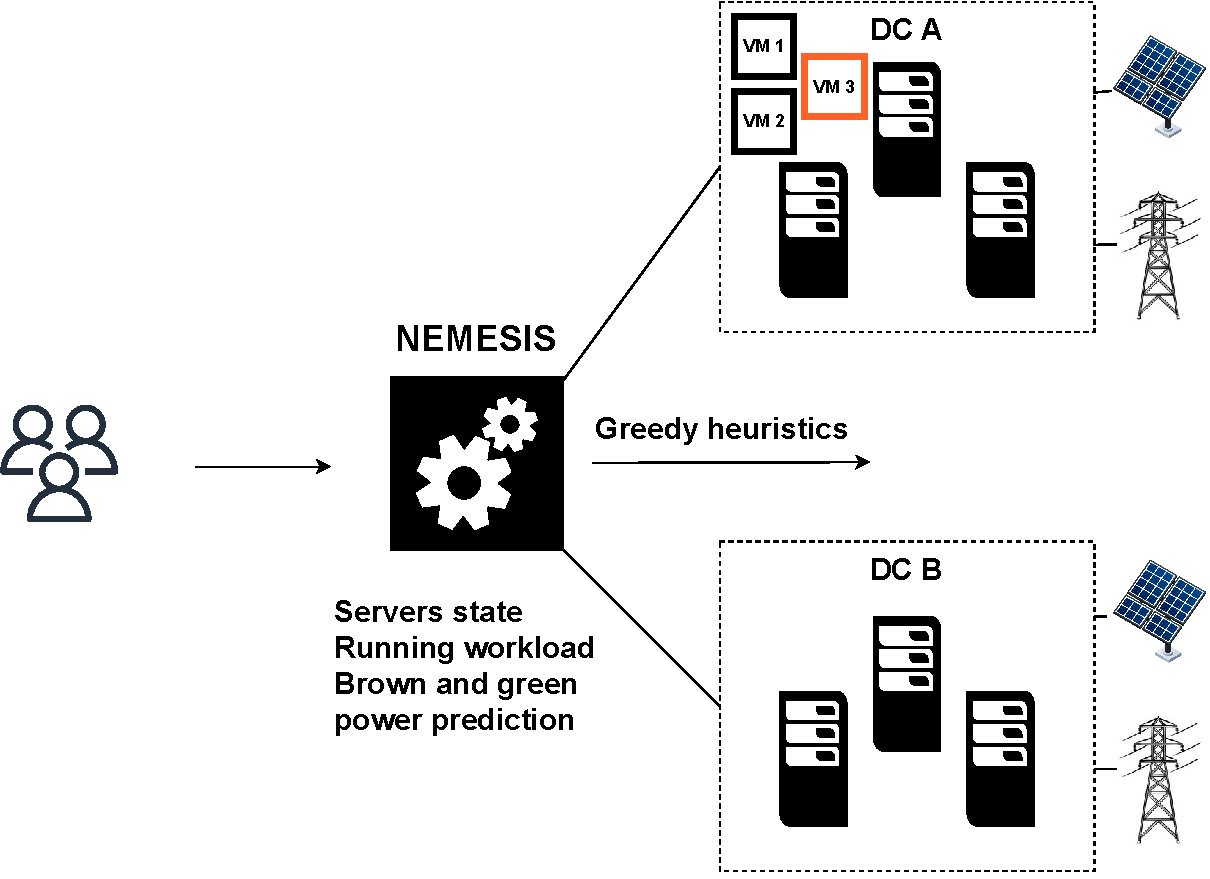
\includegraphics[width=.85\textwidth]{images/nemesis_review_2.pdf}
        \caption{NEMESIS framework.}
      \end{figure}
    \end{column}        

\end{columns}
\end{frame}



\begin{frame}{NEMESIS}
  \textbf {``\alert{N}etwork-aware \alert{E}nergy-efficient
    \alert{M}anagement framework for distribut\alert{E}d cloud\alert{S} \alert{I}nfrastructures with on-\alert{S}ite photovoltaic production''}\footfullcite{NEMESIS}
\begin{columns}        
    \begin{column}{0.4\textwidth}
Main steps:
\small
\begin{itemize}
    \item Pre-allocation of incoming Virtual Machines (VMs)
    \item Revision of pre-allocations
    \item \alert{\textbf{Migration of the running VMs}}
    \item Servers consolidation
\end{itemize}
\end{column}

\begin{column}{0.6\textwidth}
      \begin{figure}[!h]
        \centering
        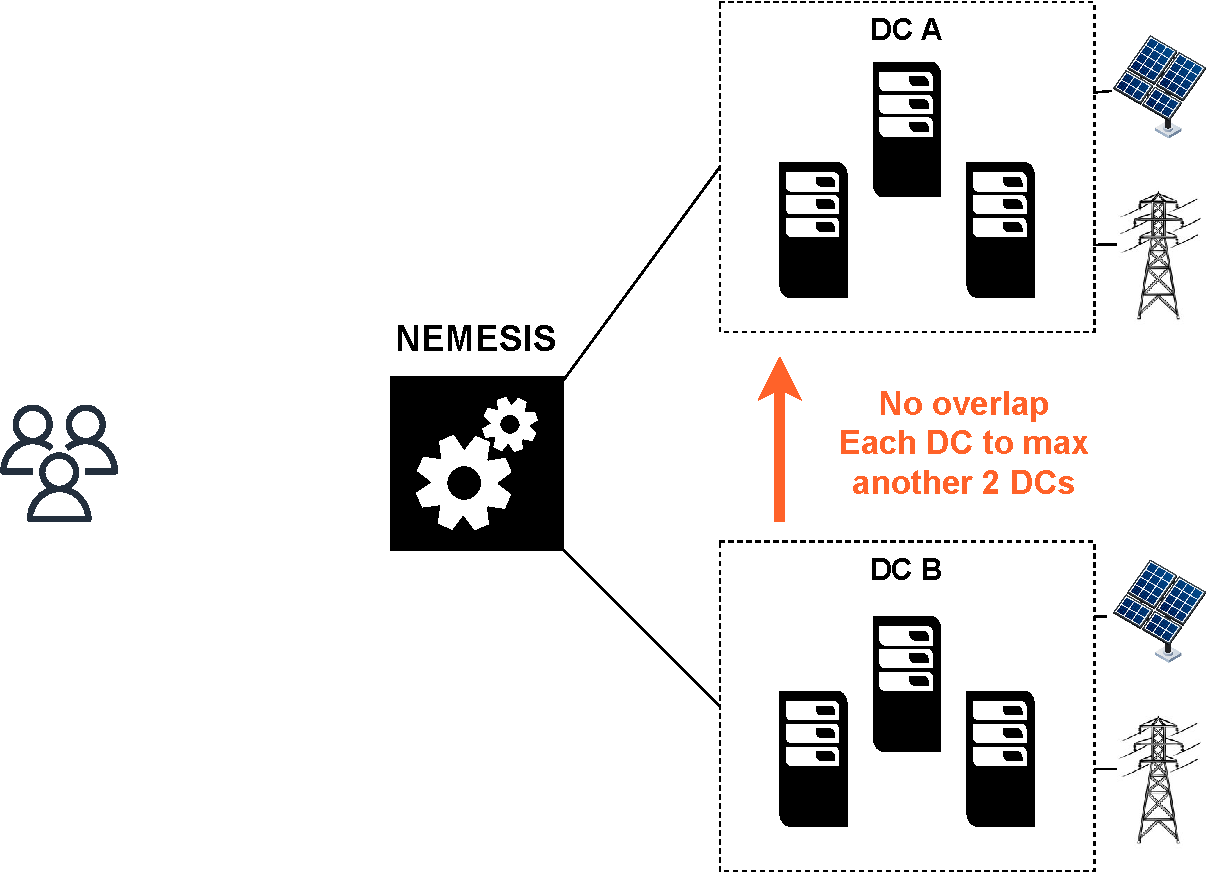
\includegraphics[width=.85\textwidth]{images/nemesis_migration.pdf}
        \caption{NEMESIS framework.}
      \end{figure}
    \end{column}        

\end{columns}
\end{frame}


\begin{frame}{NEMESIS}
  \textbf {``\alert{N}etwork-aware \alert{E}nergy-efficient
    \alert{M}anagement framework for distribut\alert{E}d cloud\alert{S} \alert{I}nfrastructures with on-\alert{S}ite photovoltaic production''}\footfullcite{NEMESIS}
\begin{columns}        
    \begin{column}{0.4\textwidth}
Main steps:
\small
\begin{itemize}
    \item Pre-allocation of incoming Virtual Machines (VMs)
    \item Revision of pre-allocations
    \item Migration of the running VMs
    \item \alert{\textbf{Servers consolidation}}
\end{itemize}
\end{column}

\begin{column}{0.6\textwidth}
      \begin{figure}[!h]
        \centering
        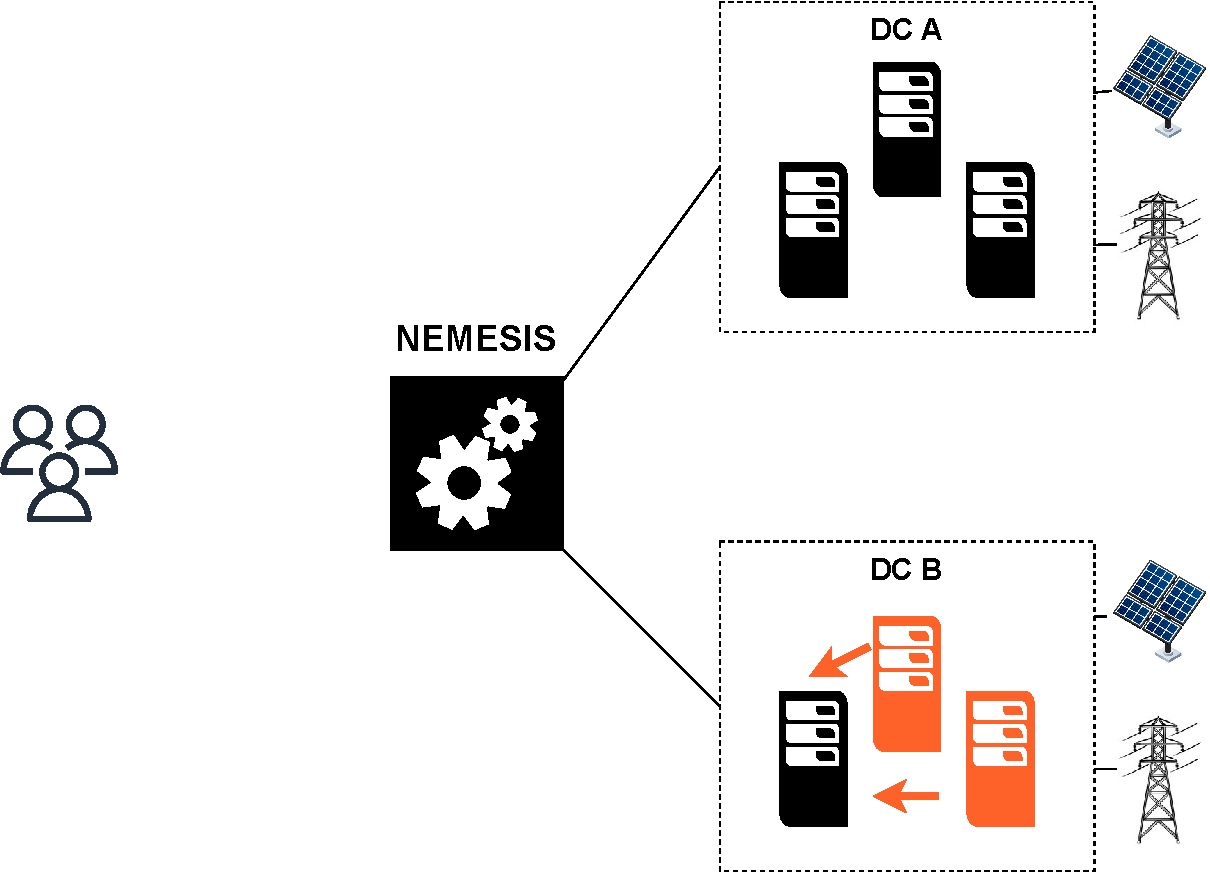
\includegraphics[width=.85\textwidth]{images/nemesis_server_consolidation.pdf}
        \caption{NEMESIS framework.}
      \end{figure}
    \end{column}        
\end{columns}
\end{frame}

\addtocounter{framenumber}{-1}

\begin{frame}{NEMESIS}
  \textbf {``\alert{N}etwork-aware \alert{E}nergy-efficient
    \alert{M}anagement framework for distribut\alert{E}d cloud\alert{S} \alert{I}nfrastructures with on-\alert{S}ite photovoltaic production''}\footfullcite{NEMESIS}
\begin{columns}        
    \begin{column}{0.4\textwidth}
Main steps:
\small
\begin{itemize}
    \item Pre-allocation of incoming Virtual Machines (VMs)
    \item Revision of pre-allocations
    \item Migration of the running VMs
    \item \alert{\textbf{Servers consolidation}}
\end{itemize}
\end{column}

\begin{column}{0.6\textwidth}
      \begin{figure}[!h]
        \centering
        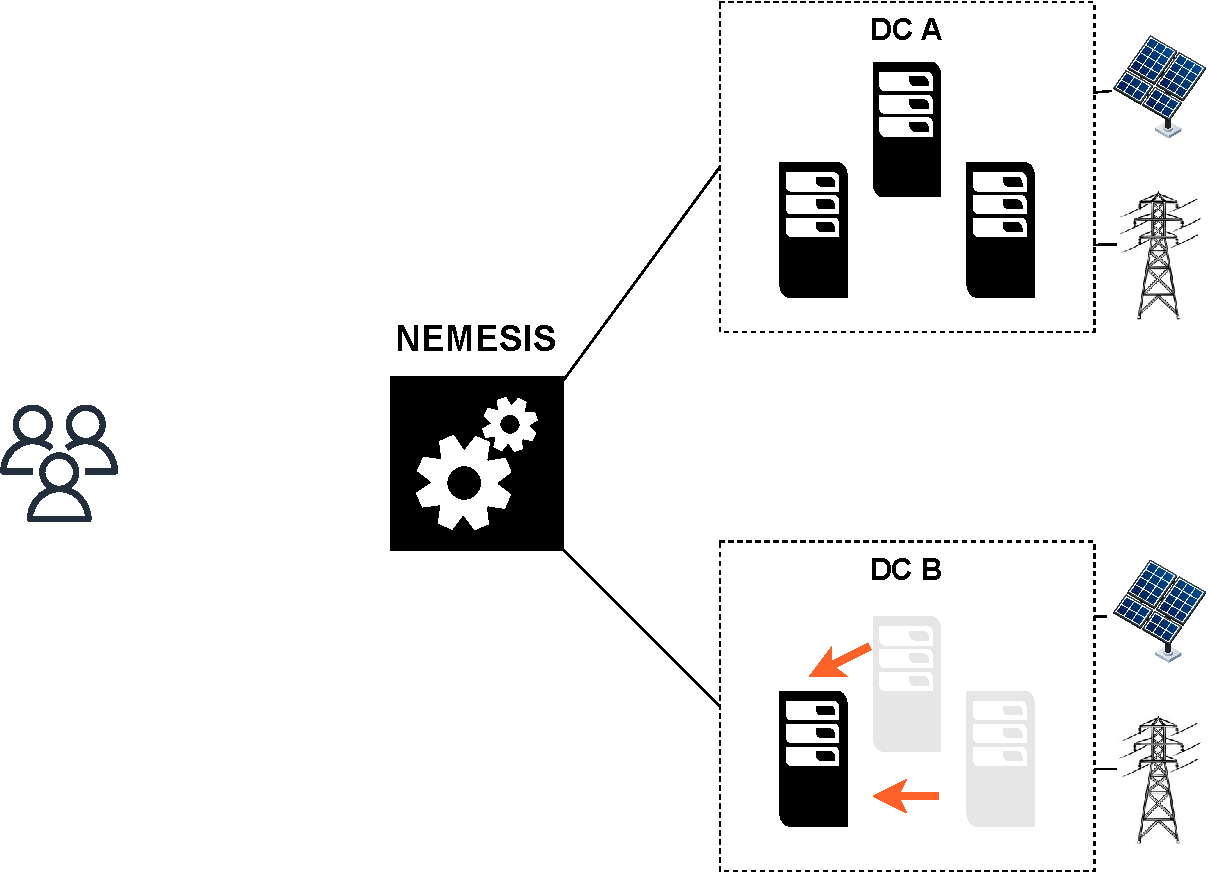
\includegraphics[width=.85\textwidth]{images/nemesis_server_consolidation_2.pdf}
        \caption{NEMESIS framework.}
      \end{figure}
    \end{column}        

\end{columns}
\end{frame}

\begin{frame}{NEMESIS}
  \textbf {``\alert{N}etwork-aware \alert{E}nergy-efficient
    \alert{M}anagement framework for distribut\alert{E}d cloud\alert{S} \alert{I}nfrastructures with on-\alert{S}ite photovoltaic production''}\footfullcite{NEMESIS}
\begin{columns}        
    \begin{column}{0.4\textwidth}
\alert{\textbf{Steps extended:}}
\small
\begin{itemize}
    \item Pre-allocation of incoming Virtual Machines (VMs)
    \item Revision of pre-allocations
    \item \alert{\textbf{Migration of the running VMs}}
    \item \alert{\textbf{Servers consolidation}}
\end{itemize}
\end{column}

\begin{column}{0.6\textwidth}
      \begin{figure}[!h]
        \centering
        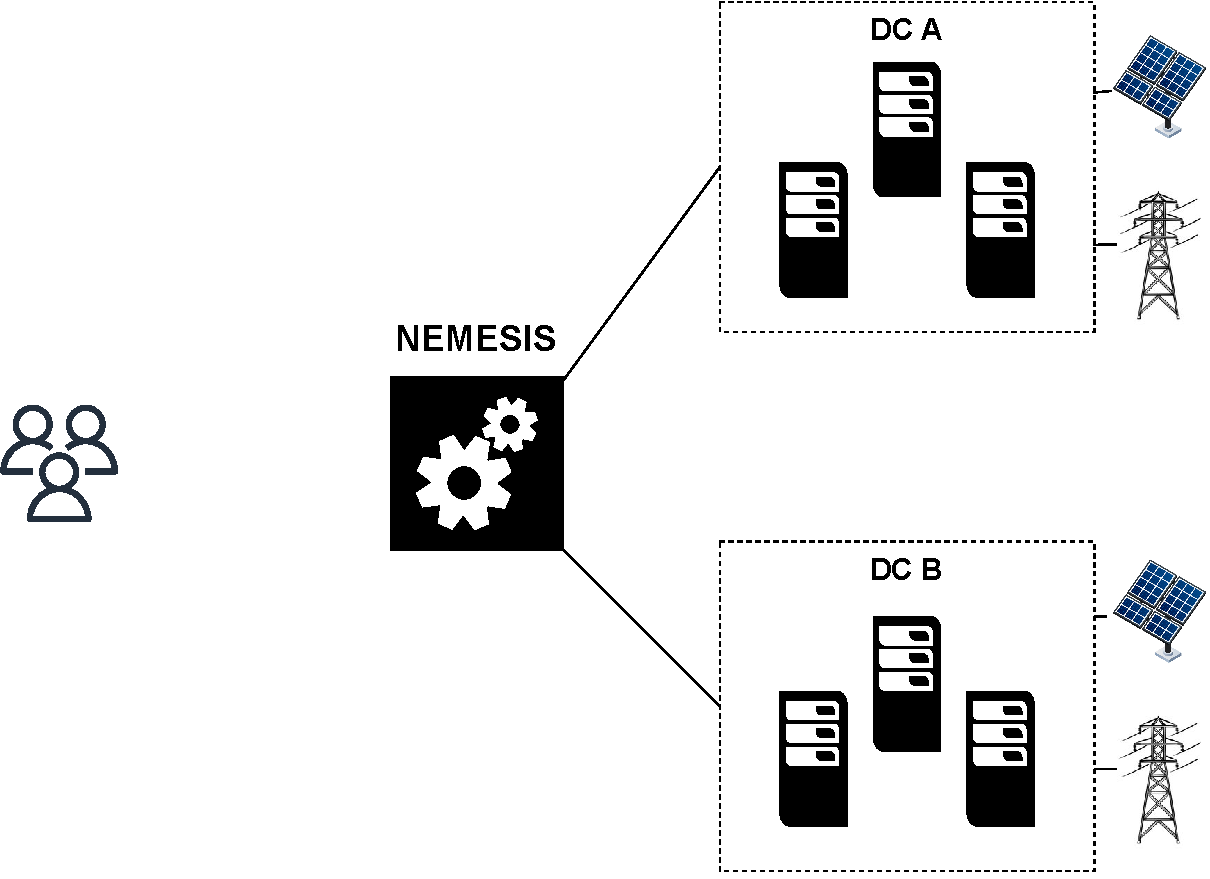
\includegraphics[width=.85\textwidth]{images/nemesis.pdf}
        \caption{NEMESIS framework.}
      \end{figure}
    \end{column}        

\end{columns}
\end{frame}

\begin{frame}{c-NEMESIS}  
  \textbf {``\alert{Congestion} and \alert{N}etwork-aware \alert{E}nergy-efficient
    \alert{M}anagement framework for distribut\alert{E}d cloud\alert{S} \alert{I}nfrastructures with on-\alert{S}ite photovoltaic production''}\footfullcite{smartgreens22}
  \begin{columns}        
    \begin{column}{0.7\textwidth}
\small
\textbf{Modifications:}
\begin{itemize}
    \item Bandwidth and usage of links
    \item Network topology
    \item Migrations for server consolidation distributed in time (no overlap)

  \end{itemize}
  
\end{column}   

\begin{column}{0.3\textwidth}
      \begin{figure}[!h]
        \centering
        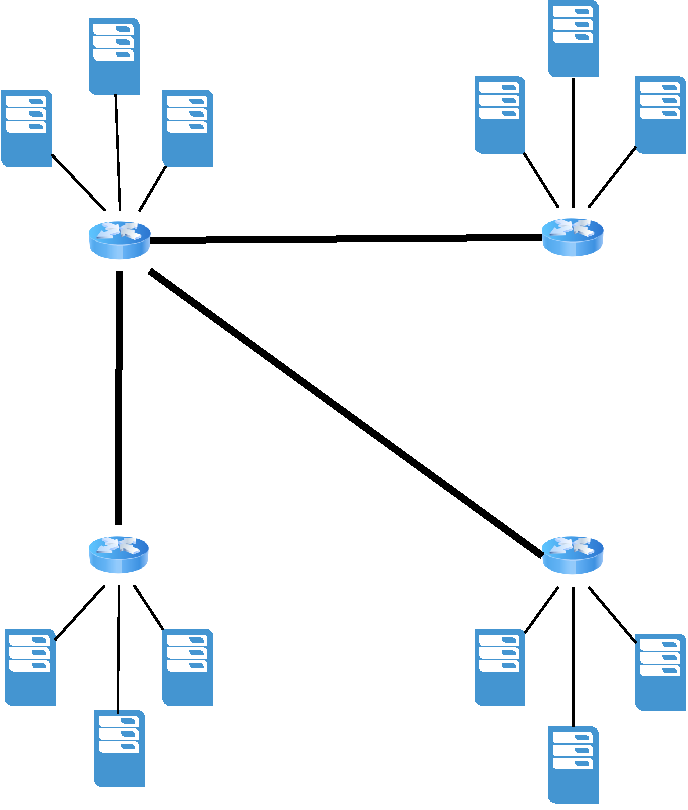
\includegraphics[width=.9\textwidth]{images/cnemesis_1.pdf}
        \caption{c-NEMESIS example.}
      \end{figure}
    \end{column}        

\end{columns}

\end{frame}

\addtocounter{framenumber}{-1}

\begin{frame}{c-NEMESIS}  
  \textbf {``\alert{Congestion} and \alert{N}etwork-aware \alert{E}nergy-efficient
    \alert{M}anagement framework for distribut\alert{E}d cloud\alert{S} \alert{I}nfrastructures with on-\alert{S}ite photovoltaic production''}\footfullcite{smartgreens22}
  \begin{columns}        
    \begin{column}{0.7\textwidth}
\small
\textbf{Modifications:}
\begin{itemize}
    \item Bandwidth and usage of links
    \item Network topology
    \item Migrations for server consolidation distributed in time (no overlap)

  \end{itemize}
  
\end{column}   

\begin{column}{0.3\textwidth}
      \begin{figure}[!h]
        \centering
        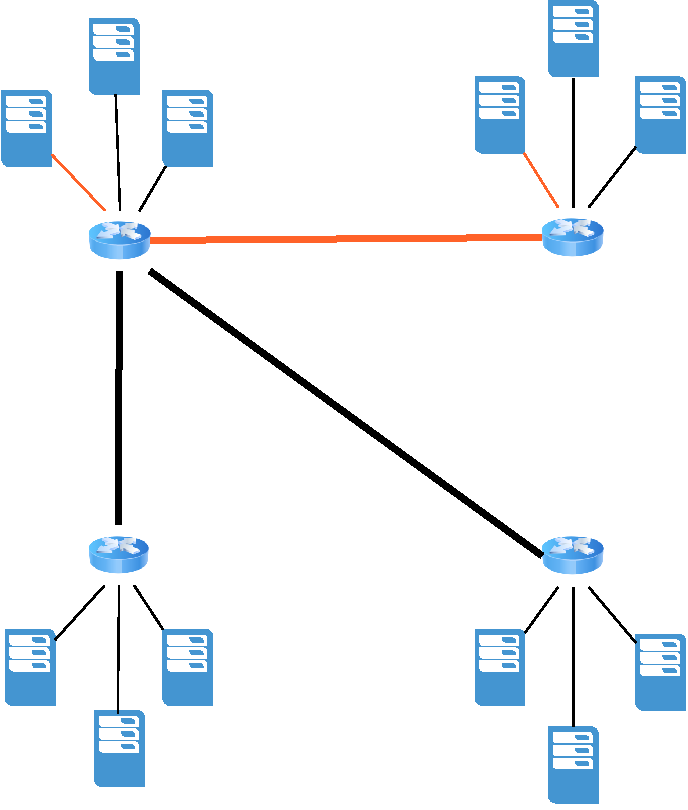
\includegraphics[width=.9\textwidth]{images/cnemesis_2.pdf}
        \caption{c-NEMESIS example.}
      \end{figure}
    \end{column}        

\end{columns}

\end{frame}
\addtocounter{framenumber}{-1}


\begin{frame}{c-NEMESIS}  
  \textbf {``\alert{Congestion} and \alert{N}etwork-aware \alert{E}nergy-efficient
    \alert{M}anagement framework for distribut\alert{E}d cloud\alert{S} \alert{I}nfrastructures with on-\alert{S}ite photovoltaic production''}\footfullcite{smartgreens22}
  \begin{columns}        
    \begin{column}{0.7\textwidth}
\small
\textbf{Modifications:}
\begin{itemize}
    \item Bandwidth and usage of links
    \item Network topology
    \item Migrations for server consolidation distributed in time (no overlap)

  \end{itemize}
  
\end{column}   

\begin{column}{0.3\textwidth}
      \begin{figure}[!h]
        \centering
        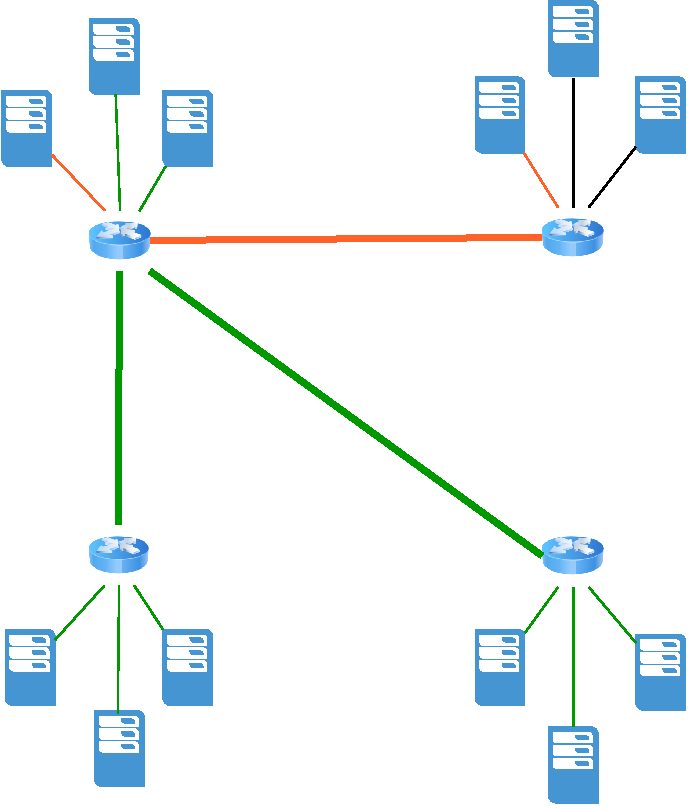
\includegraphics[width=.9\textwidth]{images/cnemesis_3.pdf}
        \caption{c-NEMESIS example.}
      \end{figure}
    \end{column}        

\end{columns}

\end{frame}

\addtocounter{framenumber}{-1}

\begin{frame}{c-NEMESIS}  
  \textbf {``\alert{Congestion} and \alert{N}etwork-aware \alert{E}nergy-efficient
    \alert{M}anagement framework for distribut\alert{E}d cloud\alert{S} \alert{I}nfrastructures with on-\alert{S}ite photovoltaic production''}\footfullcite{smartgreens22}
  \begin{columns}        
    \begin{column}{0.7\textwidth}
\small
\textbf{Modifications:}
\begin{itemize}
    \item Bandwidth and usage of links
    \item Network topology
    \item Migrations for server consolidation distributed in time (no overlap)

  \end{itemize}
  
\end{column}   

\begin{column}{0.3\textwidth}
      \begin{figure}[!h]
        \centering
        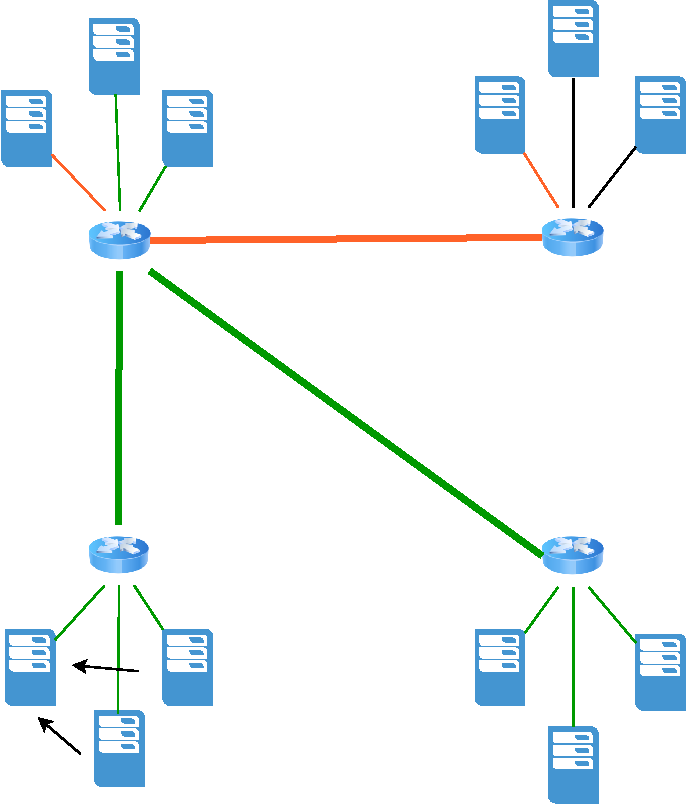
\includegraphics[width=.9\textwidth]{images/cnemesis_4.pdf}
        \caption{c-NEMESIS example.}
      \end{figure}
    \end{column}        

\end{columns}

\end{frame}

\begin{frame}{Assessing network congestion}
  \begin{columns}        
\begin{column}{0.6\textwidth}
  \begin{itemize}    
  \item \textbf{\alert{``Perfect scenario''}}:
  \begin{itemize}    
  \item full access to network resources
  \end{itemize}
  \item Additional time the migration takes vs the perfect scenario    
 \item Link under congestion:  migration 10\% longer vs  ``perfect scenario''
  \end{itemize}
\end{column}        
\begin{column}{0.4\textwidth}
  \begin{center}
    \begin{figure}[!h]
      \centering
      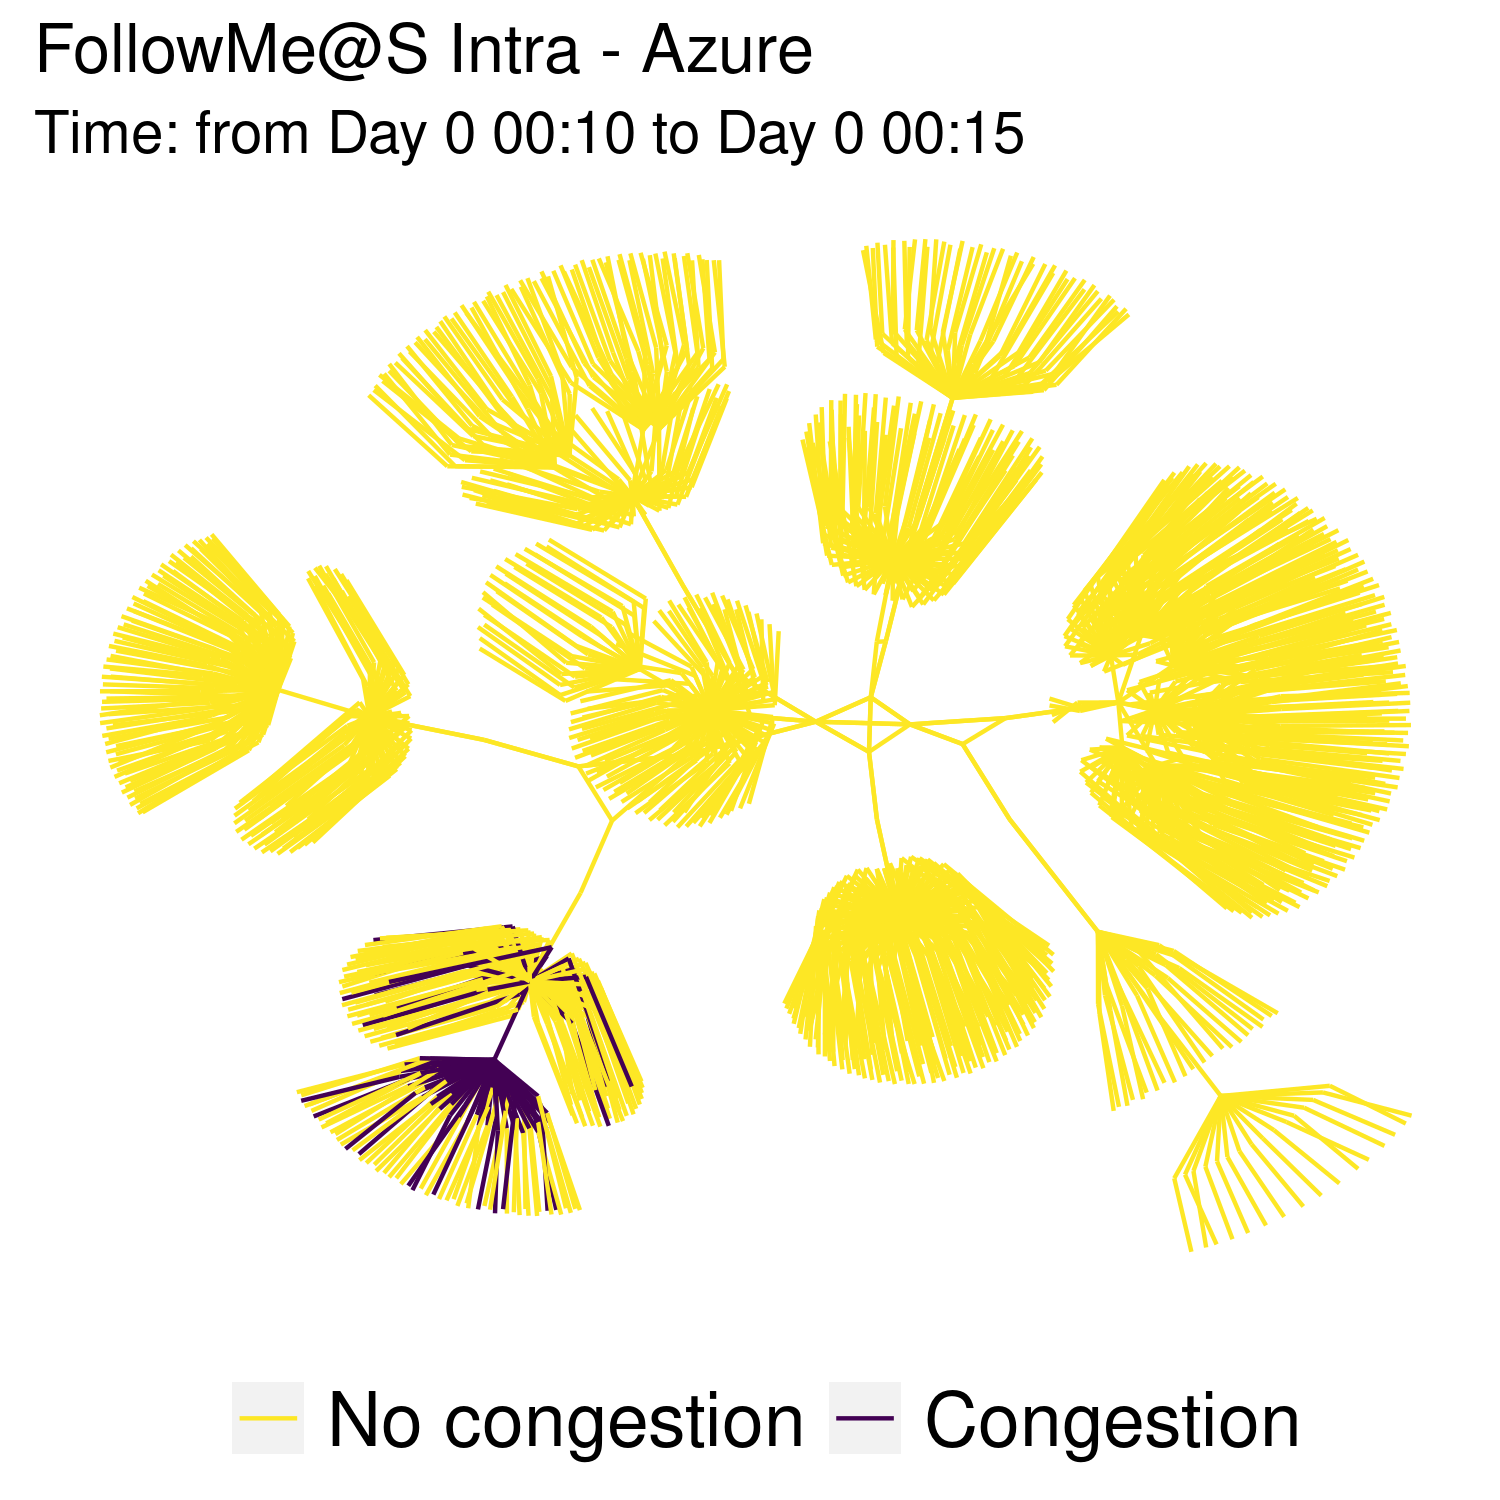
\includegraphics[width=\textwidth]{images/example_congestion.png}
      \caption{Example of links with congestion.}
    \end{figure}
  \end{center}

    \end{column}        
\end{columns}


        \end{frame}


{ % all template changes are local to this group.
    \setbeamertemplate{navigation symbols}{}
    \begin{frame}<article:0>[plain]
        \begin{tikzpicture}[remember picture,overlay]

            \node[at=(current page.center)] {
  
    \movie[width=9cm, height =9cm,autostart]{}{migrations.mp4}
  
            };
        \end{tikzpicture}
  \tikz[overlay, remember picture,
    shift=(current page.south west),
    x=(current page.south east), y=(current page.north west),
  ]{
    \node[align=left]at (0.89,0.1) {
        \small
    Network not considered\\Duration:\\ avg=4.4, max=25.56 }; 
    % Optional help grid lines
    %\draw[step=.1, opacity=0.3, thick, red] (0,0) grid (1,1);
  }
  \tikz[overlay, remember picture,
    shift=(current page.south east),
    x=(current page.south west), y=(current page.north east),
  ]{
    \node[align=left]at (0.89,0.1) {
    \small
    Network not considered\\Duration:\\ avg=7.8, max=157.24 }; 
    % Optional help grid lines
    %\draw[step=.1, opacity=0.3, thick, red] (0,0) grid (1,1);
  }
  
  \tikz[overlay, remember picture,
    shift=(current page.north east),
    x=(current page.north west), y=(current page.south east),
  ]{
    \node[align=left]at (0.9,0.15) {
    \small
    Network considered\\Bandwidth, Usage\\Topology\\Duration:\\ avg=1.0, max=1.32 }; 
    % Optional help grid lines
    %\draw[step=.1, opacity=0.3, thick, red] (0,0) grid (1,1);
  }
 \tikz[overlay, remember picture,
    shift=(current page.north west),
    x=(current page.north east), y=(current page.south west),
  ]{
    \node[align=left]at (0.89,0.15) {
        \small
    Network considered\\No overlap, 1 DC\\ to max other 2 DCs\\Duration:\\ avg=1.6, max=3.98 }; 
    % Optional help grid lines
    %\draw[step=.1, opacity=0.3, thick, red] (0,0) grid (1,1);
  }
  
     \end{frame}
}


\begin{frame}{Wasted and non-renewable energy}  
  \begin{itemize}
  \item Wasted energy proportional to the extra time speding migrating in comparison to the perfect scenario
  \item \alert{367 kWh} of green energy was wasted in the case of the
    FollowMe@S Intra algorithm with the Google workload
  \item This energy could have powered the one of the DCs \alert{(38 servers at maximum capacity)}  for approximately \alert{ 44 hours}
  
  \end{itemize}
  
\end{frame}



\begin{frame}{Total and brown energy consumption}  
  \begin{table}[!h]
    \caption{Comparison of energy consumption (MWh) for the Azure workload.}\label{tab:total_energy_cons} \centering
    \begin{tabular}{|l|r|r|}      
      \hline
      \textbf{Algorithm} & \textbf{Total} &  \textbf{Non-renewable} \\
      \hline
      c-NEMESIS & 30.55 & 21.20 \\
      \hline
      NEMESIS  & 30.43 & 21.21 \\ 
            \hline
      FollowMe@S Inter & 31.69 & 22.40 \\

      \hline
      FollowMe@S Intra & 31.69 & 22.41 \\
      \hline
      WSNB & 33.56 & 24.23 \\
      \hline
    \end{tabular}
  \end{table}  
\end{frame}



\begin{frame}{Summary - first main contribution of this thesis}
    \begin{itemize}
    \item Bad migration planning results in network congestion, waste of renewable energy (and increase in non-renewable energy consumption)
    \item Follow-the-renewables approaches need to consider all the workload execution, given the intermittent nature of renewables
    \end{itemize} \pause

\textbf{Modern cloud DCs are geographically distributed all over the world, not all DCs have on-site renewable infrastructure, and some locations already have presence of renewable sources, how to reduce the carbon footprint in this scenario?}

\end{frame}

\section{Model for sizing the renewable and IT infrastructure and operating the DCs}



\begin{frame}{Sizing the renewable and IT infrastructure}  


  \begin{columns}        
\begin{column}{0.5\textwidth}
  \begin{itemize}
  \item Defining:  
  
  \begin{itemize}
  \item Area of solar panels
  %\item Number of wind turbines
  \item Capacity of energy storage devices %and servers
  \end{itemize}

\item{Considerations:}
\begin{itemize}
  \item Climate conditions
  \item Energy-mix
  \item Carbon footprint of renewable sources %and renewable %and servers,  servers hardware specifications
\end{itemize}
\end{itemize}
\end{column}        
\begin{column}{0.5\textwidth}
  \begin{center}
    \begin{figure}[!h]
      \centering
      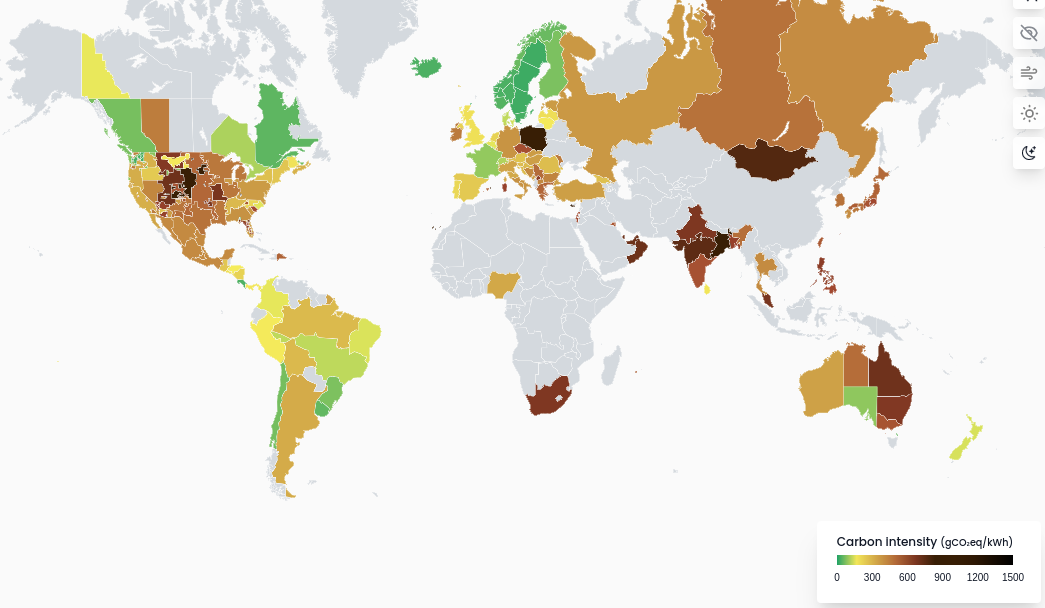
\includegraphics[width=\textwidth]{images/electricity_map.png}
      \caption{Electricitymap service.}
    \end{figure}

  \end{center}

    \end{column}        
\end{columns}


\end{frame}




\begin{frame}{Proposed solution}
 
  Linear program formulation to minimize the carbon emissions from the cloud federation operation (timespan of 1 year) \footnotemark[2]
  
  \begin{itemize}
    
  \item Scheduling and sizing modeled as single problem
    \begin{itemize}
      
    \item Allocate workload to other DC or increase the \textbf{battery capacity} or \textbf{solar panels} (PV) area?
    \end{itemize}
    
  \item Only real variables 
    \begin{itemize}     
    \item  Optimal solution in polynomial time

    \end{itemize}

  \end{itemize}
    
  \footnotetext[2]{M. Vasconcelos, D. Cordeiro, G. Da Costa, F. Dufossé, J.-M. Nicod, and V. Rehn-Sonigo, ``Optimal sizing of a globally distributed low carbon cloud federation''. \textit{In: 2023 23nd IEEE International Symposium on Cluster, Cloud and Internet Computing (CCGrid), Bengaluru, India, 2023.}}
\end{frame}

\begin{frame}{Data centers modeling}  

\begin{columns}
    \begin{column}{.5\textwidth}
        
  
  \begin{itemize}

  \item Infrastructure already built (servers, network)
  \item Homogeneous (regarding CPU cores)
  \item Server power consumption: idle and dynamic 
  \item Intra-network power consumption: static 
  \item Specific Power Usage Effectiveness (PUE) for each DC

  \end{itemize}
    \end{column}
    \begin{column}{.5\textwidth}
  \begin{figure}[!h]
    \centering
    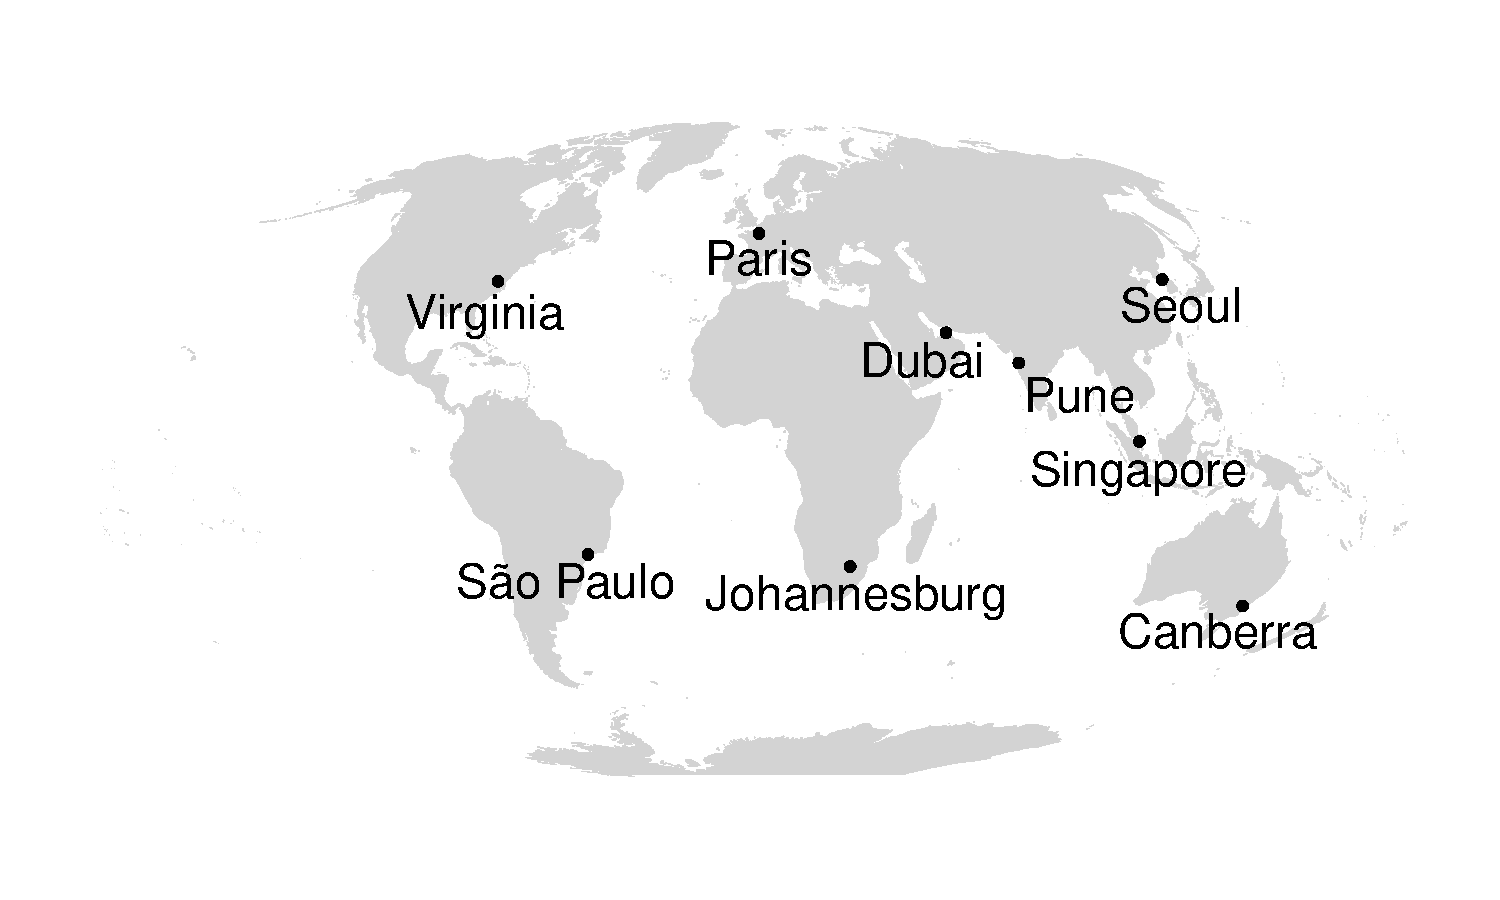
\includegraphics[width=\textwidth]{images/locations_.pdf}
    \caption{Selected data centers location (inspired from Microsoft Azure)}
  \end{figure}       
    \end{column}
\end{columns}

  

   
\end{frame}


\begin{frame}{Workload modeling}  
  \textbf{}
  
  \begin{itemize}  
  \item All tasks must be scheduled and executed on time
  \item Batch tasks that can be executed in any of the DCs 
  \item Task execution cannot be delayed
  \item No migration %\pause 
    \begin{itemize}  
    \item High network links latency, migrating a VM with 12 GB of RAM takes: min. $\approx 4$ min, avg. $\approx 14$ min, max. $\approx 49$ min
  \end{itemize}
  \end{itemize}

\end{frame}

\begin{frame}{Renewables infrastructure modeling}
  
  
  
  \begin{itemize}    
  \item Batteries charge and discharge efficiency, Maximum Depth of Discharge
  \item PV panels efficiency    
  \item Carbon emissions from manufacturing (PV: 250 kg \ch{CO2}-eq per m², bat: 59 kg \ch{CO2}-eq per kWh)
  \item Lifetime (PV: 30 years, bat: 10 years)      
  \end{itemize}
  
\end{frame}
\addtocounter{framenumber}{-1}

\begin{frame}{Local electricity grid modeling}
  
  \begin{itemize}

  \item The energy mix is different at each location
  \item May have the presence of renewables or low carbon-intensive sources    
    
    \begin{table}
      
      \caption{Carbon footprint of the regular grid at each location. Source for grid emissions: electricityMap, climate-transparency.org.}\label{tab:carbonfootprint} \centering
      \small
      \begin{tabular}{|l|r|}
        
        \hline

        \textbf{Location} &  \textbf{Emissions (g \ch{CO2}-eq per kWh)}  \\
        \hline
        Johannesburg & 900.6  \\
        \hline
        Pune & 702.8\\
        \hline
        Canberra & 667.0 \\
        \hline
        Dubai & 530.0   \\
        \hline
        Singapore & 495.0  \\
        \hline     
        Seoul & 415.6  \\
        \hline
        Virginia  & 342.8  \\
        \hline
        São Paulo &  61.7 \\
        \hline 
        Paris &  52.6  \\
        \hline  

      \end{tabular}  
    \end{table}
    
  \end{itemize}
  \normalsize
\end{frame}



\begin{frame}{LP model - DC power consumption and supply} 
  \alert{ Data center power consumption ($P^d_k $):}
  
  \begin{equation}    
    P^d_k  = PUE^d \times \big( Pintranet^d + Pidle^d  + Pcore \times w^d_k\big)
  \end{equation}

 % where $PUE^d$ is the cooling efficiency at data center $d$,
 % $Pintranet^d$ is the power consumption of the network devices,
 % $Pidle^d$ is the server static power consumption, $PCore$ the
 % dynamic power consumption of using a CPU core, and $w^d_k$ is the
 % workload allocated on DC d at time slot k .


  \alert{ Data center power supply:}
  
  \begin{equation}
    P^d_k \leq Pre^d_k + Pgrid^d_k + Pdch_k^d - Pch_k^d   
  \end{equation}


  %where $Pch_k^d$ is the power to charge the battery at each time of time slot $k$ on $DC^d$ and $Pdch_k^d$ is the power to discharge the battery, $Pre^d_k $ is the solar power produced, and $ Pgrid^d_k $ is the power used from the local grid.

\end{frame}

\begin{frame}{LP model - renewable infrastructure}

  \alert{Batteries level of energy ($B^d_ k$):} 

  \begin{equation} \label{eq:bdk}
    B^d_k = B^d_{k-1}  + Pch^d_{k-1} \times \eta_{ch} \times \Delta{t} - \frac{Pdch^d_{k-1}}{\eta_{dch}} \times \Delta{t}
  \end{equation}

%  where $\eta_{ch}$ is efficiency of the charge process and $\eta_{dch}$ is the efficiency of the discharge process.

  \alert{Solar power production:}

  \begin{equation} \label{eq:predk}
    Pre^d_{k}= I^d_k \times Apv^d \times \eta_{pv}
  \end{equation}

 % where $I^d_k$ is the solar irradiance, $Apv^d$ the PV panel area,  and $\eta_{pv}$ is the efficiency of PV module

\end{frame}



\begin{frame}{  Linear Program summary}

  \alert{Obj. function:} Minimize the DC's operation \ch{CO2} emissions (1 year 8760 time slots of 1 h)
  \small   
 \begin{equation} \label{eq:FPALL}
    \text{minimize }\sum_{k=0}^{K-1} \sum_{d=1}^D ( FPgrid^d_k +  FPpv^d_k) + \sum_{d=1}^D FPbat^d
  \end{equation}
\normalsize
  \begin{itemize}
  \item \ch{CO2} comes from: grid power, manufacturing PV and batteries
  \end{itemize}
  
  \begin{columns}[T]
    \begin{column}{0.55\textwidth}
      \pause
      \alert{Input}

      \begin{itemize}
      \item Power consumption of servers and network equipment
      \item 1 year of workload  (Google trace)
      \item Renewable infrastructure specs (efficiency, manufacturing \ch{CO2})
      \item For each DC:
        \begin{itemize}
        \item Solar irradiation (1 year), Grid \ch{CO2}, PUE, CPU cores number
        \end{itemize}
      \end{itemize}
      
    \end{column}

    \begin{column}{0.45\textwidth}
      
      \pause          
      \alert{Output}
      
      \begin{itemize}          
      \item PVs area (m²)          
      \item Batteries capacity (kWh)                  
      \item Total \ch{CO2} emissions 
      \item Schedule of the workload         
      \end{itemize}
    \end{column}
  \end{columns}      
\end{frame}




\begin{frame}{Results - \ch{CO2} emissions}
  \begin{table}[!ht]
    \caption{Total emissions for the different scenarios.}\label{tab:emissions} \centering
    \begin{tabular}{|p{5cm}|r|}
      \hline
      \textbf{Scenarios} & \textbf{Emissions (t \ch{CO2}-eq)}   \\
      \hline
      Electrical grid                    & 201 211.3    \\
      \hline
      PV and batteries  &                  42 370.6 \\ 
      \hline
      PV, batteries, and grid            &  29 600.6   \\
      \hline
    \end{tabular}
  \end{table}
\pause
    Reductions on carbon emissions:
  
  \begin{itemize}
  \item Grid vs DC renewable infra : \alert{$\simeq 5$ times}\pause
  \item Grid vs hybrid configuration (DC renewables and grid) : \alert{$\simeq 6$ times}
  \end{itemize}

\end{frame}



\begin{frame}{Results - Sizing}
  \begin{figure}[!htbp]
    \centering
    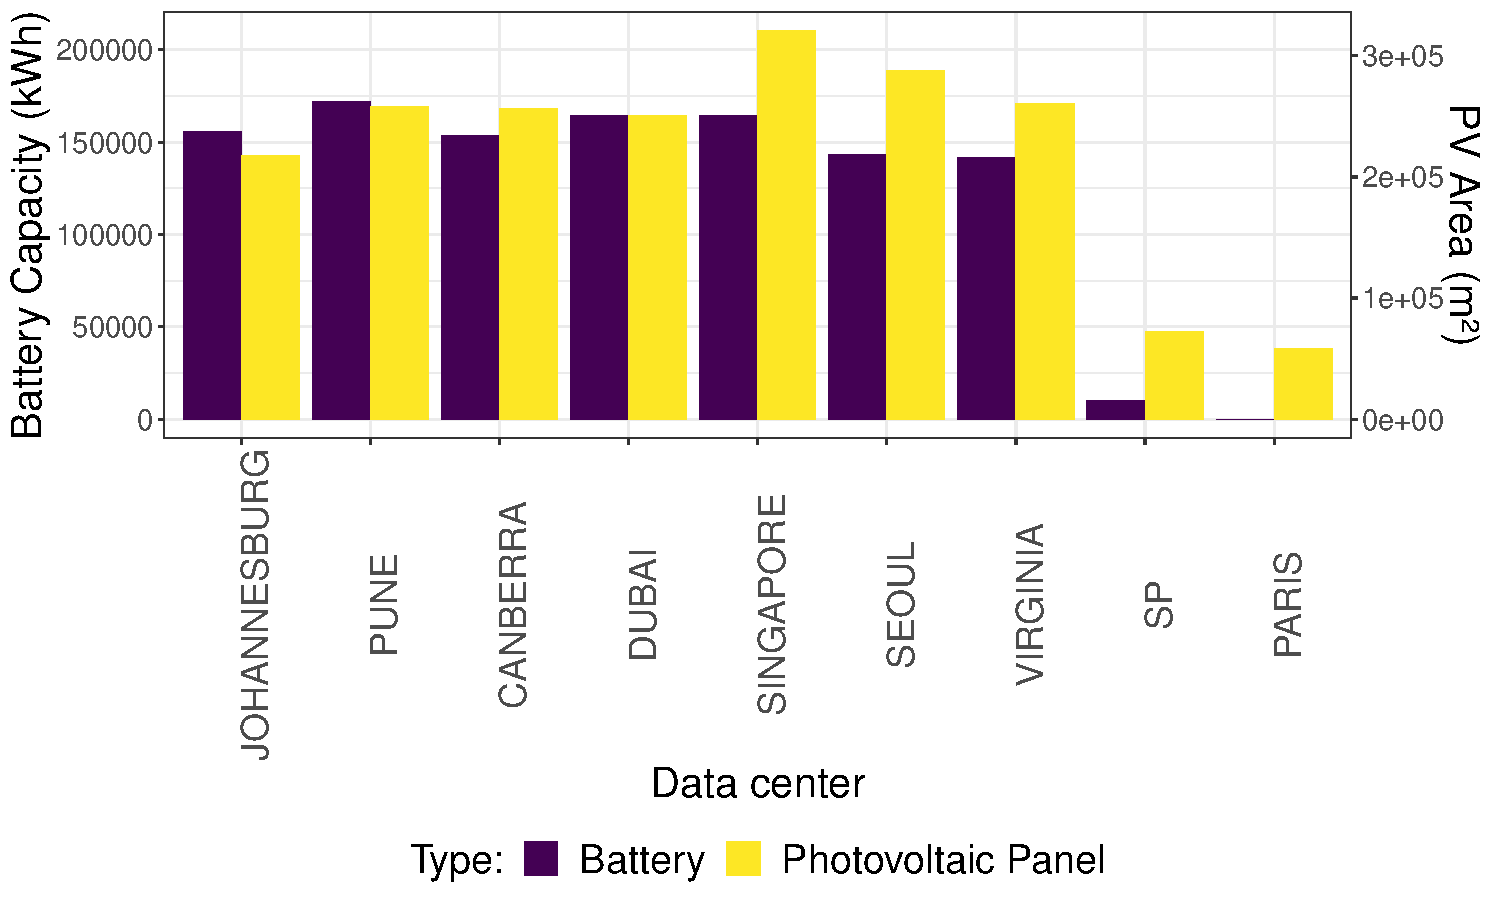
\includegraphics[width=.8\textwidth]{images/sizing.pdf}
    \caption{Optimal result for the area of PV panels and capacity of the batteries.}
    \label{fig:sizing}
  \end{figure}
\end{frame}

\begin{frame}{Visualization of DCs operation}
  
  \begin{itemize}    
  \item Each circle is a DC, and the radius is the power consumption (MW)
  \item The pizza graph represents the share of electricity source being used at that instant (PVs, batteries, or from the grid)
  \item The gray shadow represents the night
  \item Visualization for the first week of 2021
  \end{itemize}
  
  \begin{center}
    \begin{figure}[!h]
      \centering
      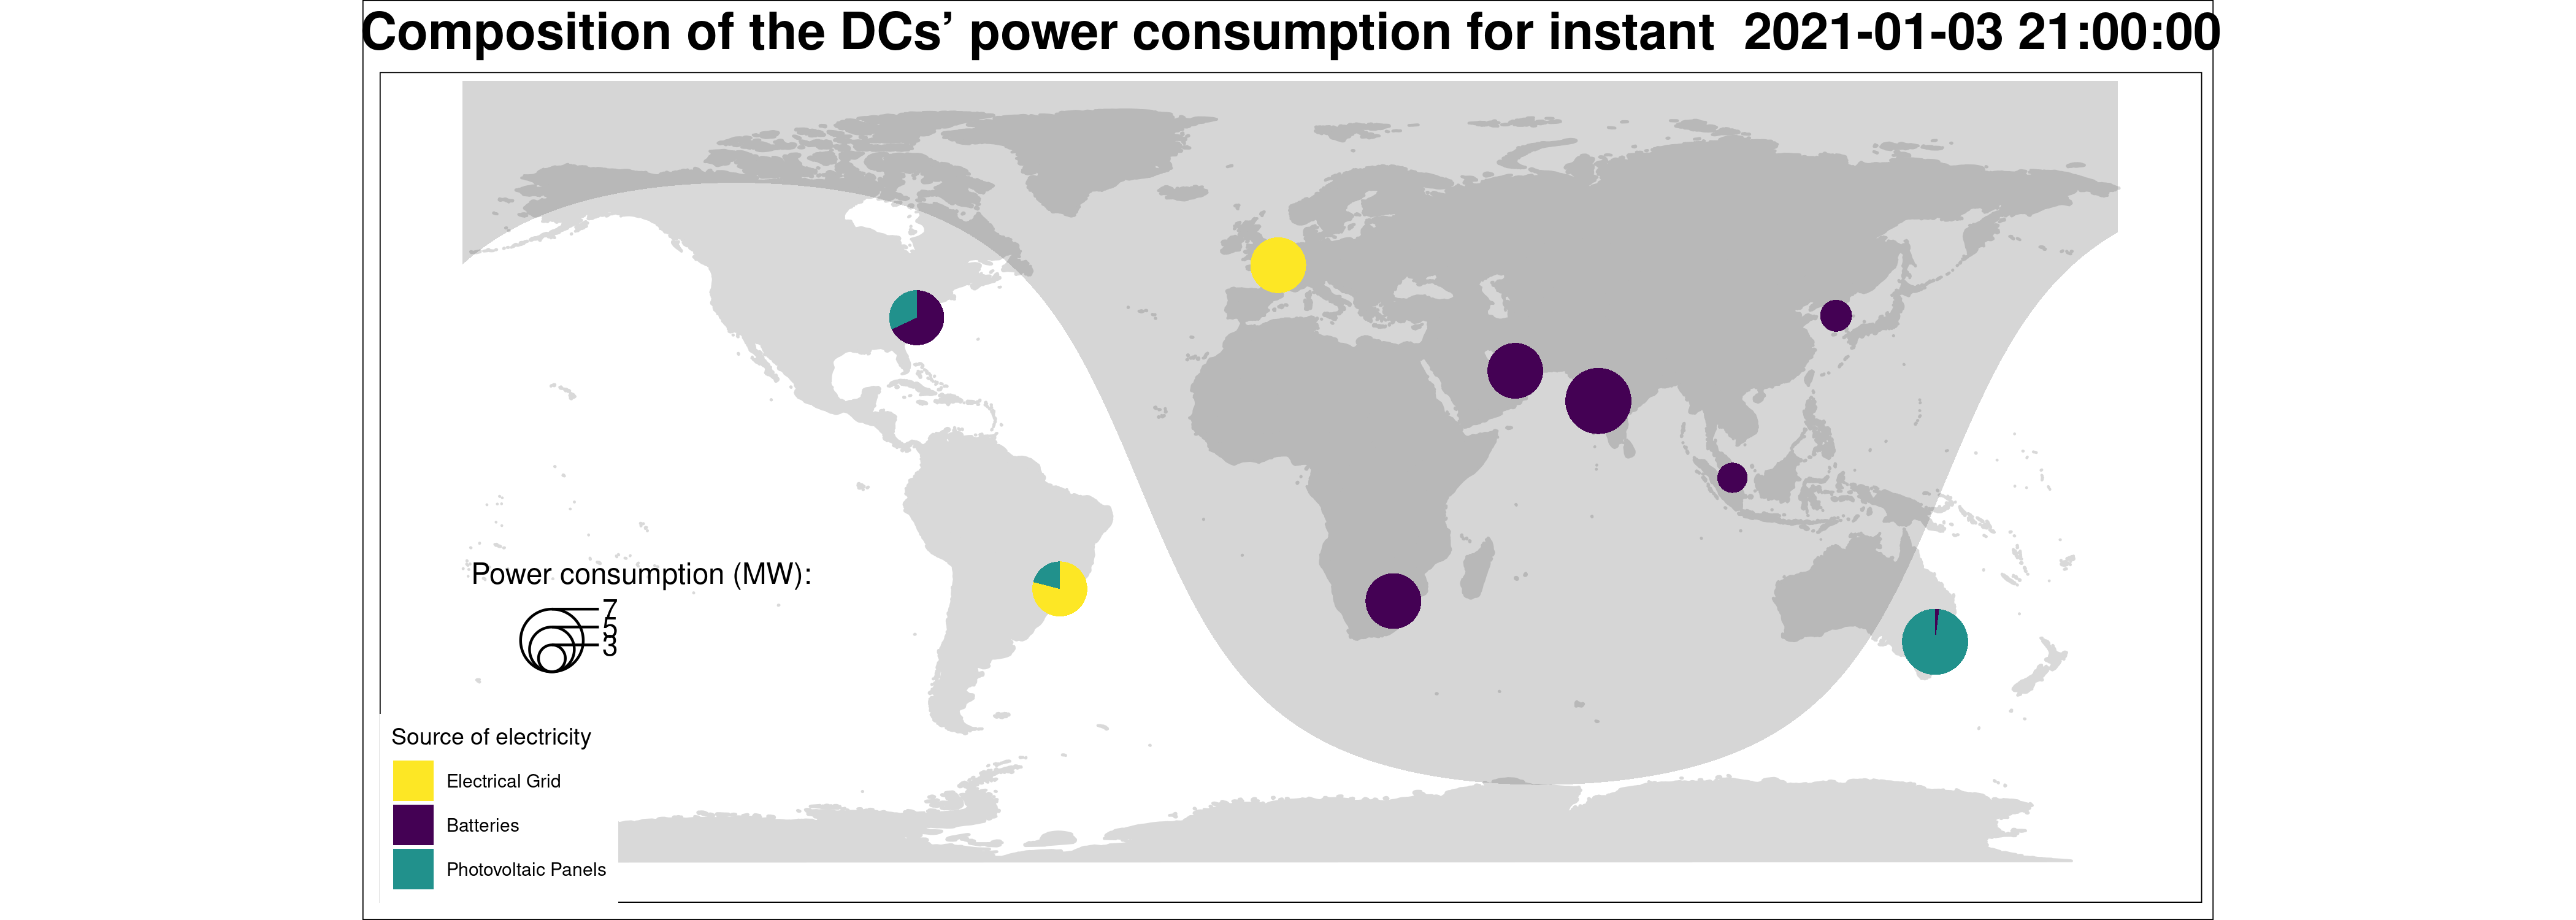
\includegraphics[width=.8\textwidth]{images/dc_op_plot.png}
      \caption{Example of data centers electricity source used.}
    \end{figure}
  \end{center}
\end{frame}
\addtocounter{framenumber}{-1}



{ % all template changes are local to this group.
    \setbeamertemplate{navigation symbols}{}
    \begin{frame}<article:0>[plain]
        \begin{tikzpicture}[remember picture,overlay]
            \node[at=(current page.center)] {
  
    \movie[width=16cm, height =16cm,loop,autostart]{}{dc_op.mp4}
  
            };
        \end{tikzpicture}
     \end{frame}
}



\begin{frame}{Sizing for the long term}

First modeling considering the short-term, but DCs have lifetime \textbf{longer than one decade} 

\begin{itemize}  
    \item Manufacturing is only one of the phases of the life cycle of renewable infrastructure
    \item Workload keep increasing over time
    \item Hardware might be more power-efficient
    
\end{itemize}  

What about?
\begin{itemize} 
  \item Wind power
  \item Delaying the workload
  \item Costs (dollars)
\end{itemize}

\end{frame}
\addtocounter{framenumber}{-1}

\begin{frame}{Sizing for the long term}

First modeling considering the short-term, but DCs have lifetime longer than one decade
\begin{itemize}  
    \item Manufacturing is only one of the phases of the life   cycle of renewable infrastructure
    \item \textbf{\alert{Workload keep increasing over time}}
    \item \textbf{\alert{Hardware might be more power-efficient}}

\end{itemize}  

What about?
\begin{itemize} 
  \item Wind power
  \item Delaying the workload
  \item \textbf{\alert{Costs (dollars)}}
\end{itemize}

\end{frame}


\begin{frame}{Costs (\$) of reducing the environmental impact}

  \begin{itemize}  
  \item   How to measure the price of the renewable infrastructure? 
  
  \begin{itemize}
  
  \item  \textbf{Levelized Cost of Energy (LCOE)}: Cost of manufacturing, operating, maintenance, related to the energy it can produce during the lifetime (\$ per kWh)
  \item  \textbf{Levelized Cost of Storage (LCOS)}: Cost of manufacturing, operating, maintenance, related to the energy it is possible to discharge during the lifetime (\$ per kWh)
  
  \end{itemize}
      
  \end{itemize}
 
 
\end{frame}

\addtocounter{framenumber}{-1}

\begin{frame}{Costs (\$) of reducing the environmental impact}
  \begin{itemize}
  
  \item   Considered the Levelized Cost of Energy for the renewables
%  \item   Values computed using models, and parameters from the NREL
  \item   Grid price is half at off-peak times (10 pm to 8 am)
  \item   Battery price: 0.20 dollars per kWh of electricity delivered
  
  \end{itemize}
  \begin{figure}[!htbp]
    \centering
    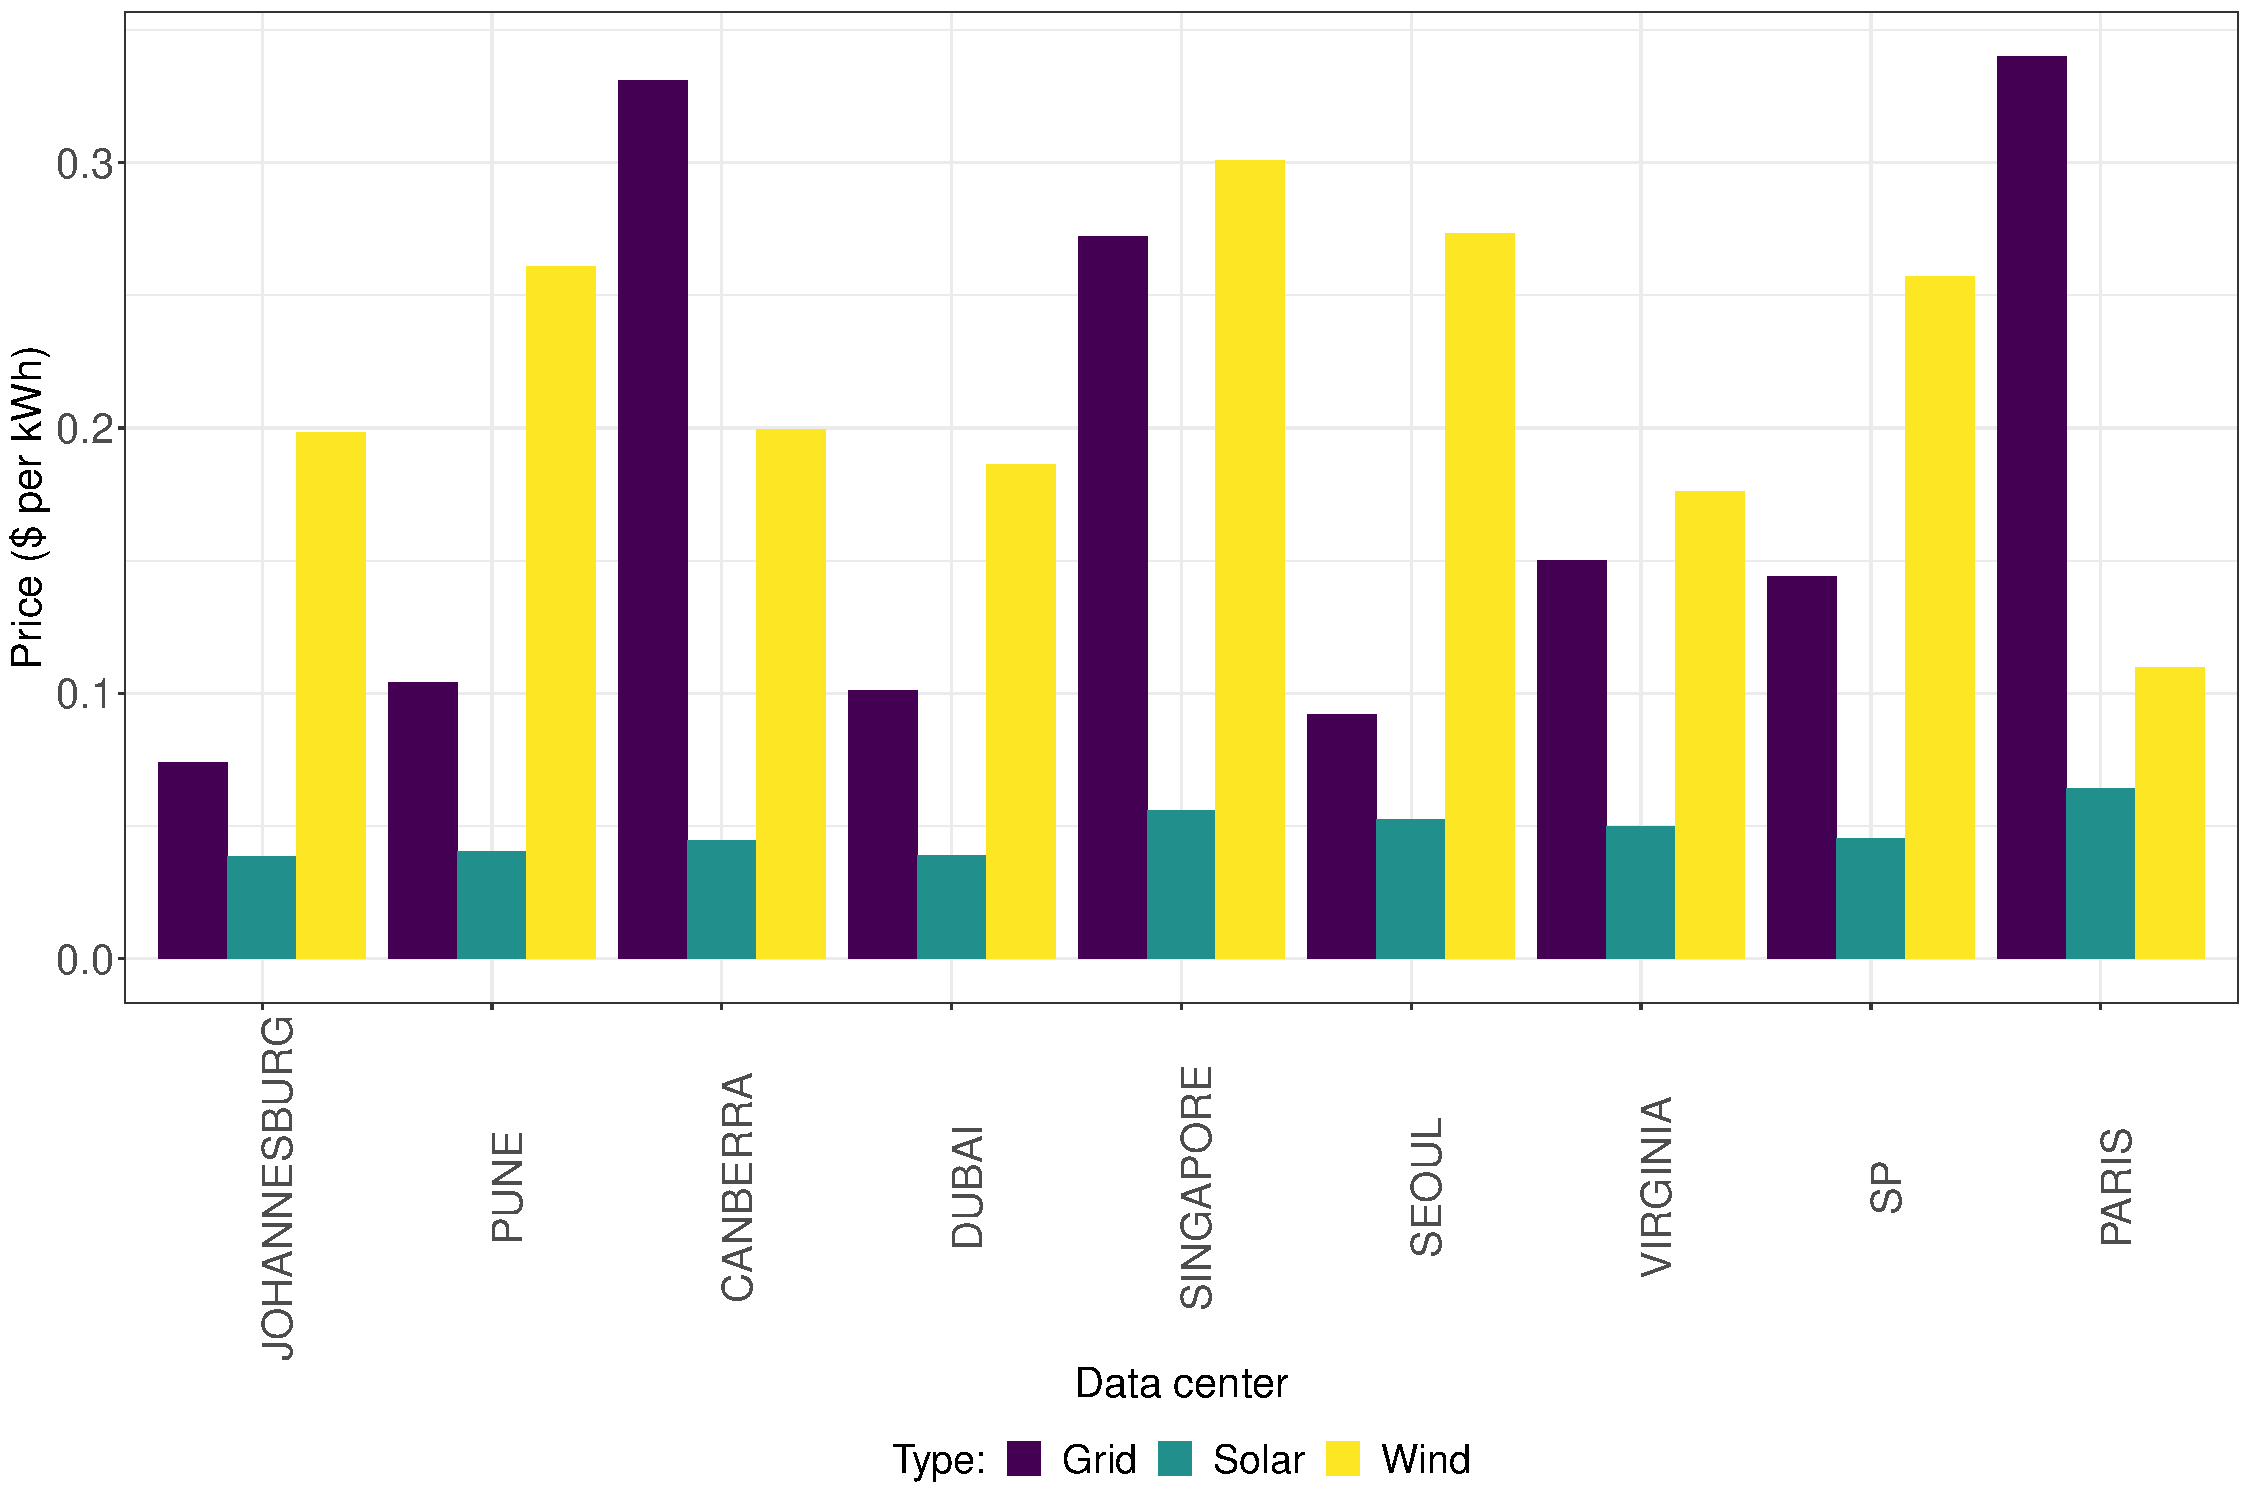
\includegraphics[width=.65\textwidth]{images/price_electricity.pdf}
    \caption{Price of different sources of energy (USD per kWh) at each location.}
    \label{fig:sizing}
  \end{figure}
  
\end{frame}


\begin{frame}{Costs (\$) of reducing the environmental impact}


\begin{figure}[h]
\centering
  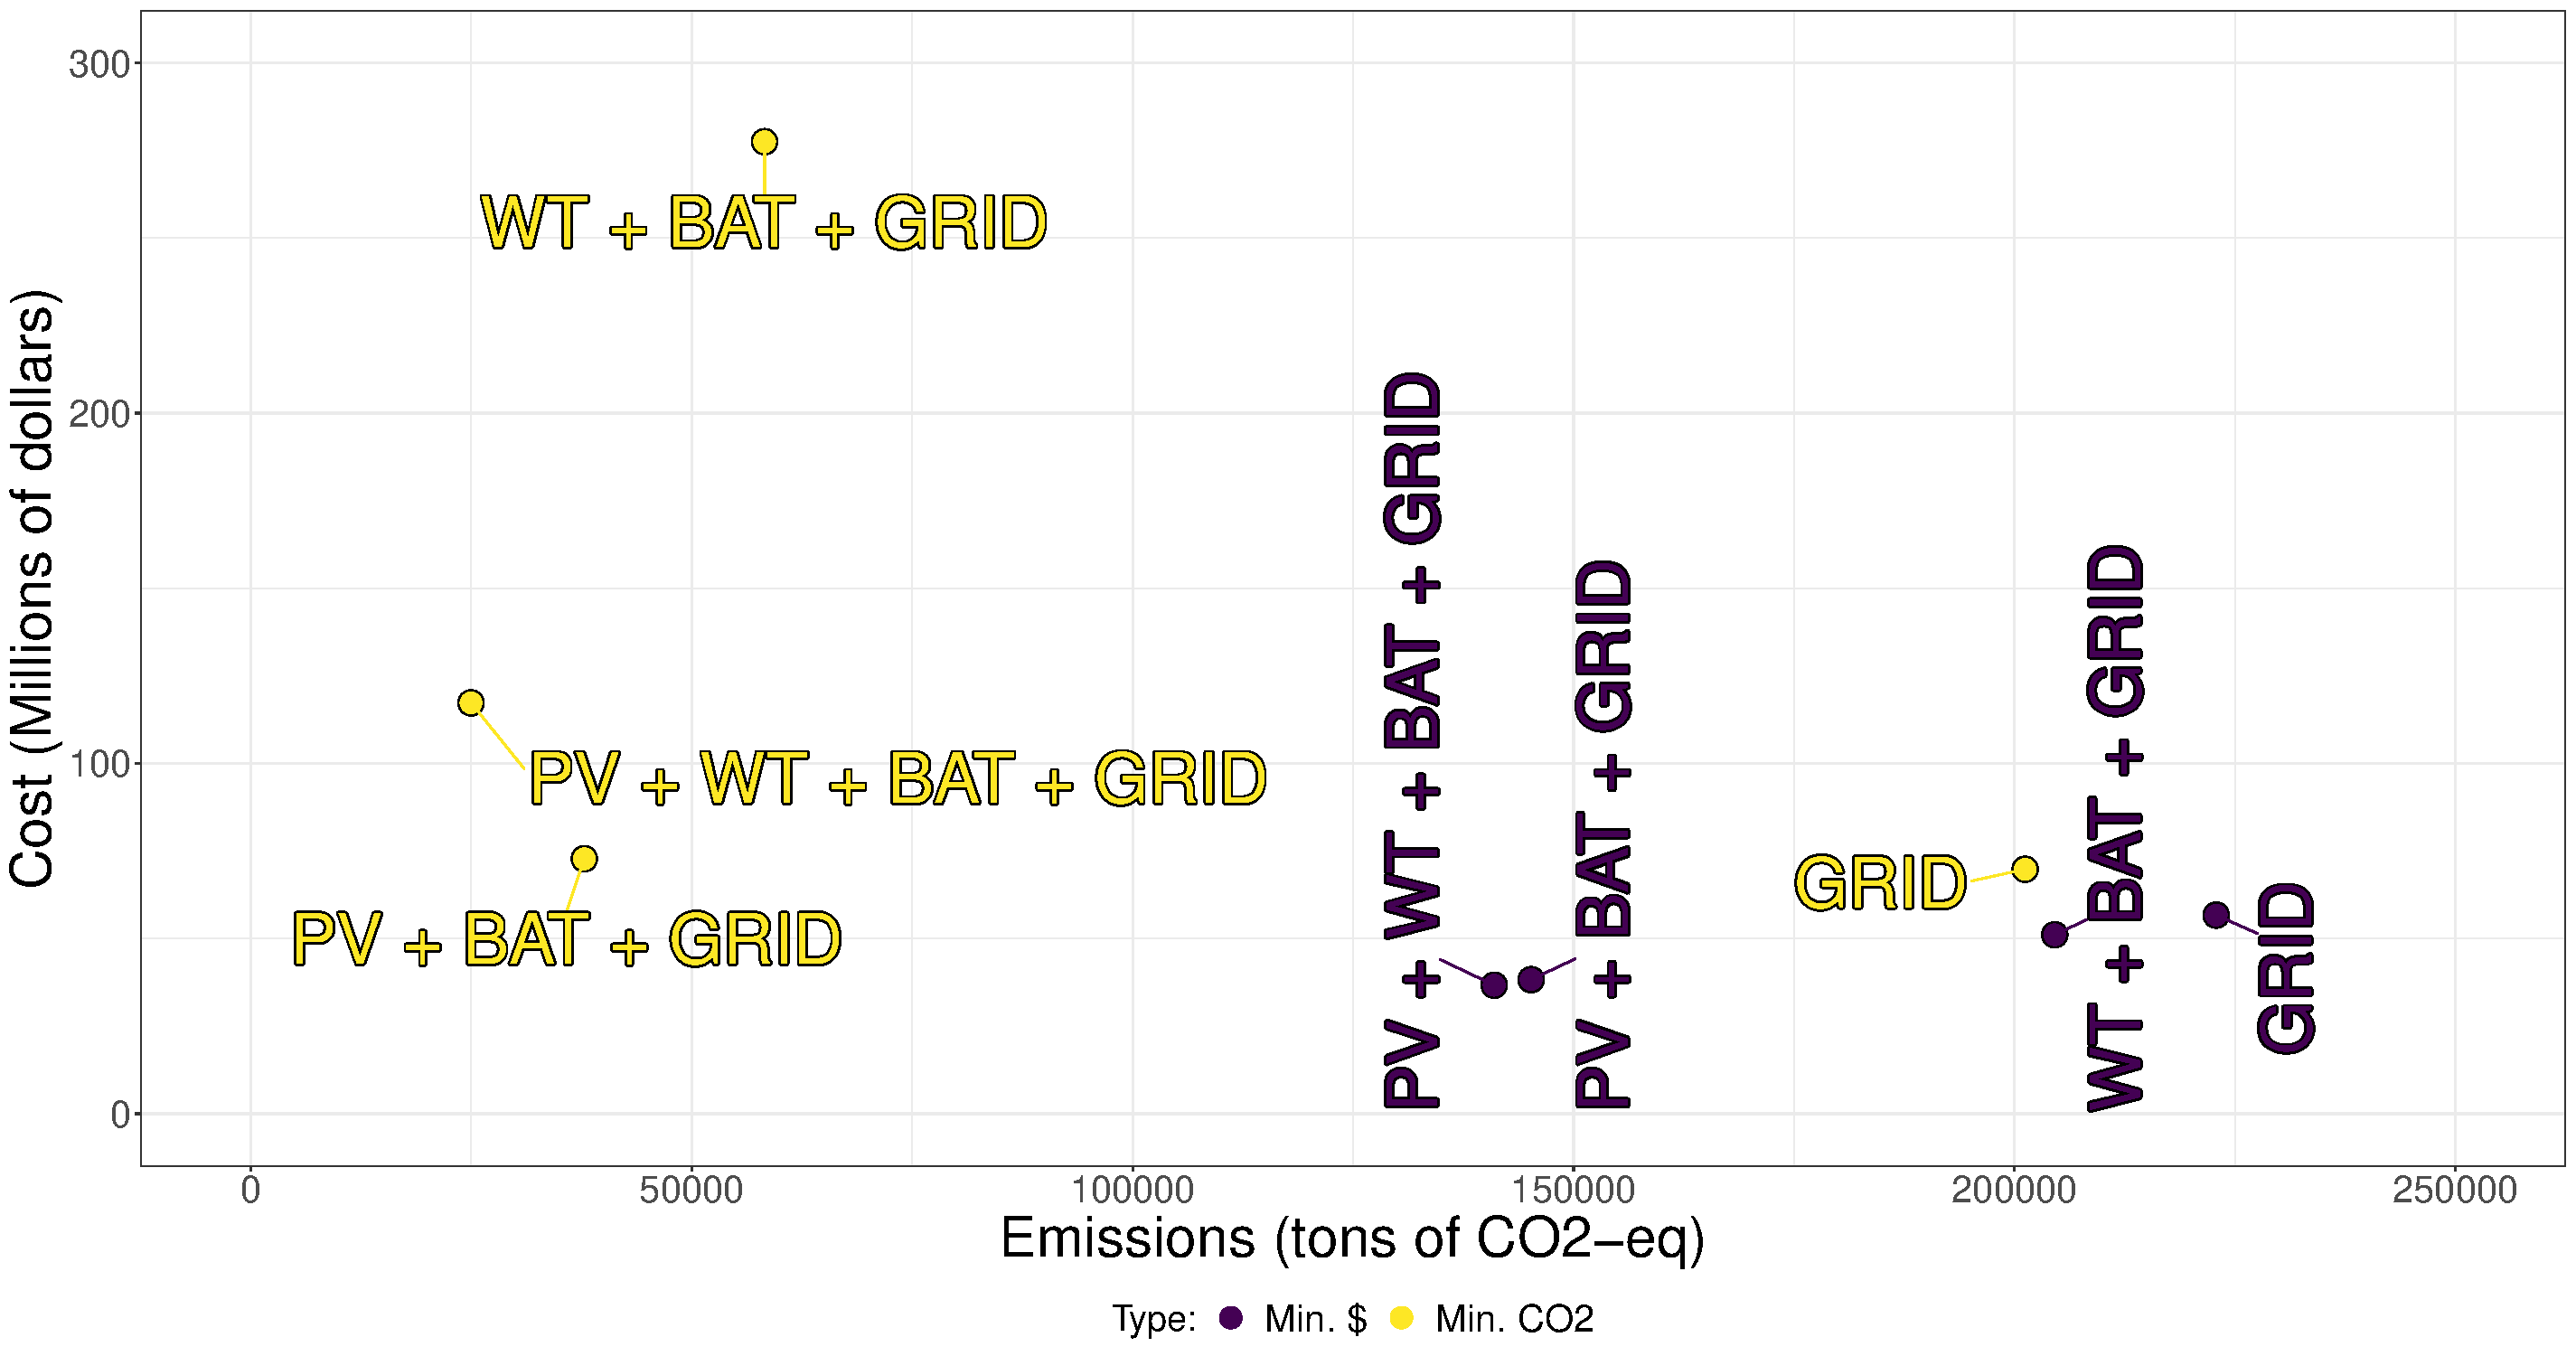
\includegraphics[width=.9\textwidth]{images/costs_vs_co2_scenarios.pdf}
  \caption{Costs vs \ch{CO2} emissions for the different scenarios.}
\end{figure}


\end{frame}

\addtocounter{framenumber}{-1}

\begin{frame}{Costs (\$) of reducing the environmental impact}


\begin{figure}[h]
\centering
  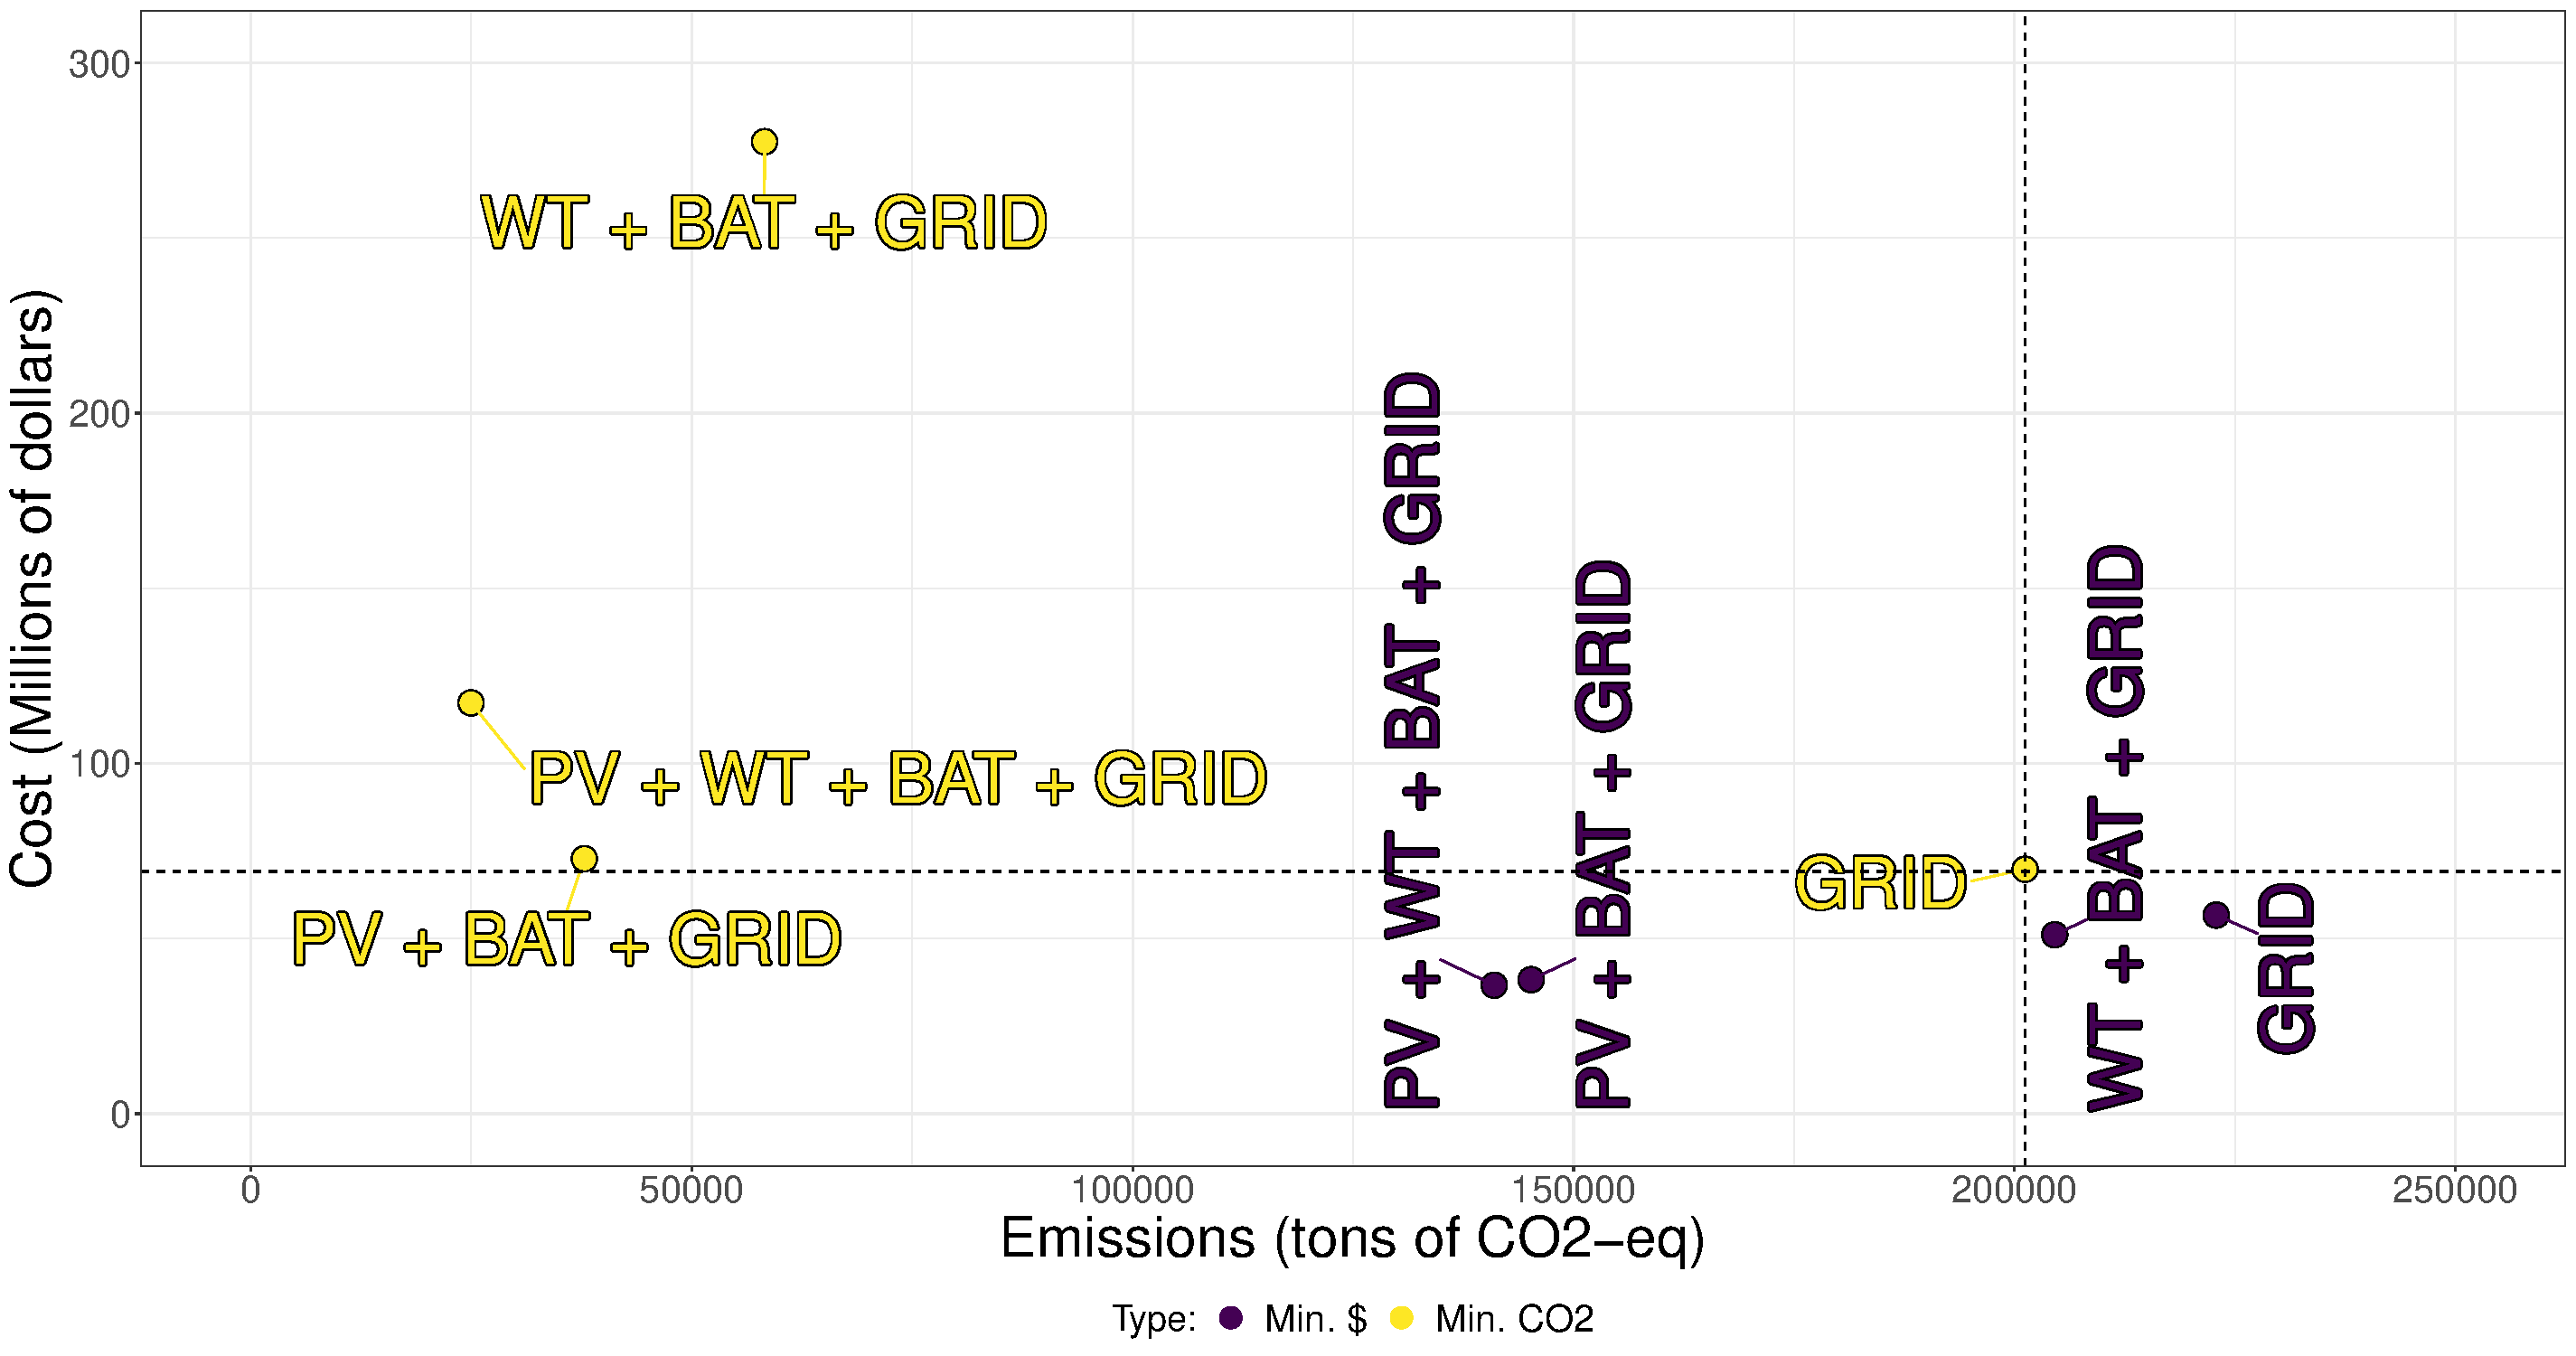
\includegraphics[width=.9\textwidth]{images/costs_vs_co2_scenarios_only_grid_co2.pdf}
  \caption{Costs vs \ch{CO2} emissions for the different scenarios.}
\end{figure}


\end{frame}


\addtocounter{framenumber}{-1}

\begin{frame}{Costs (\$) of reducing the environmental impact}


\begin{figure}[h]
\centering
  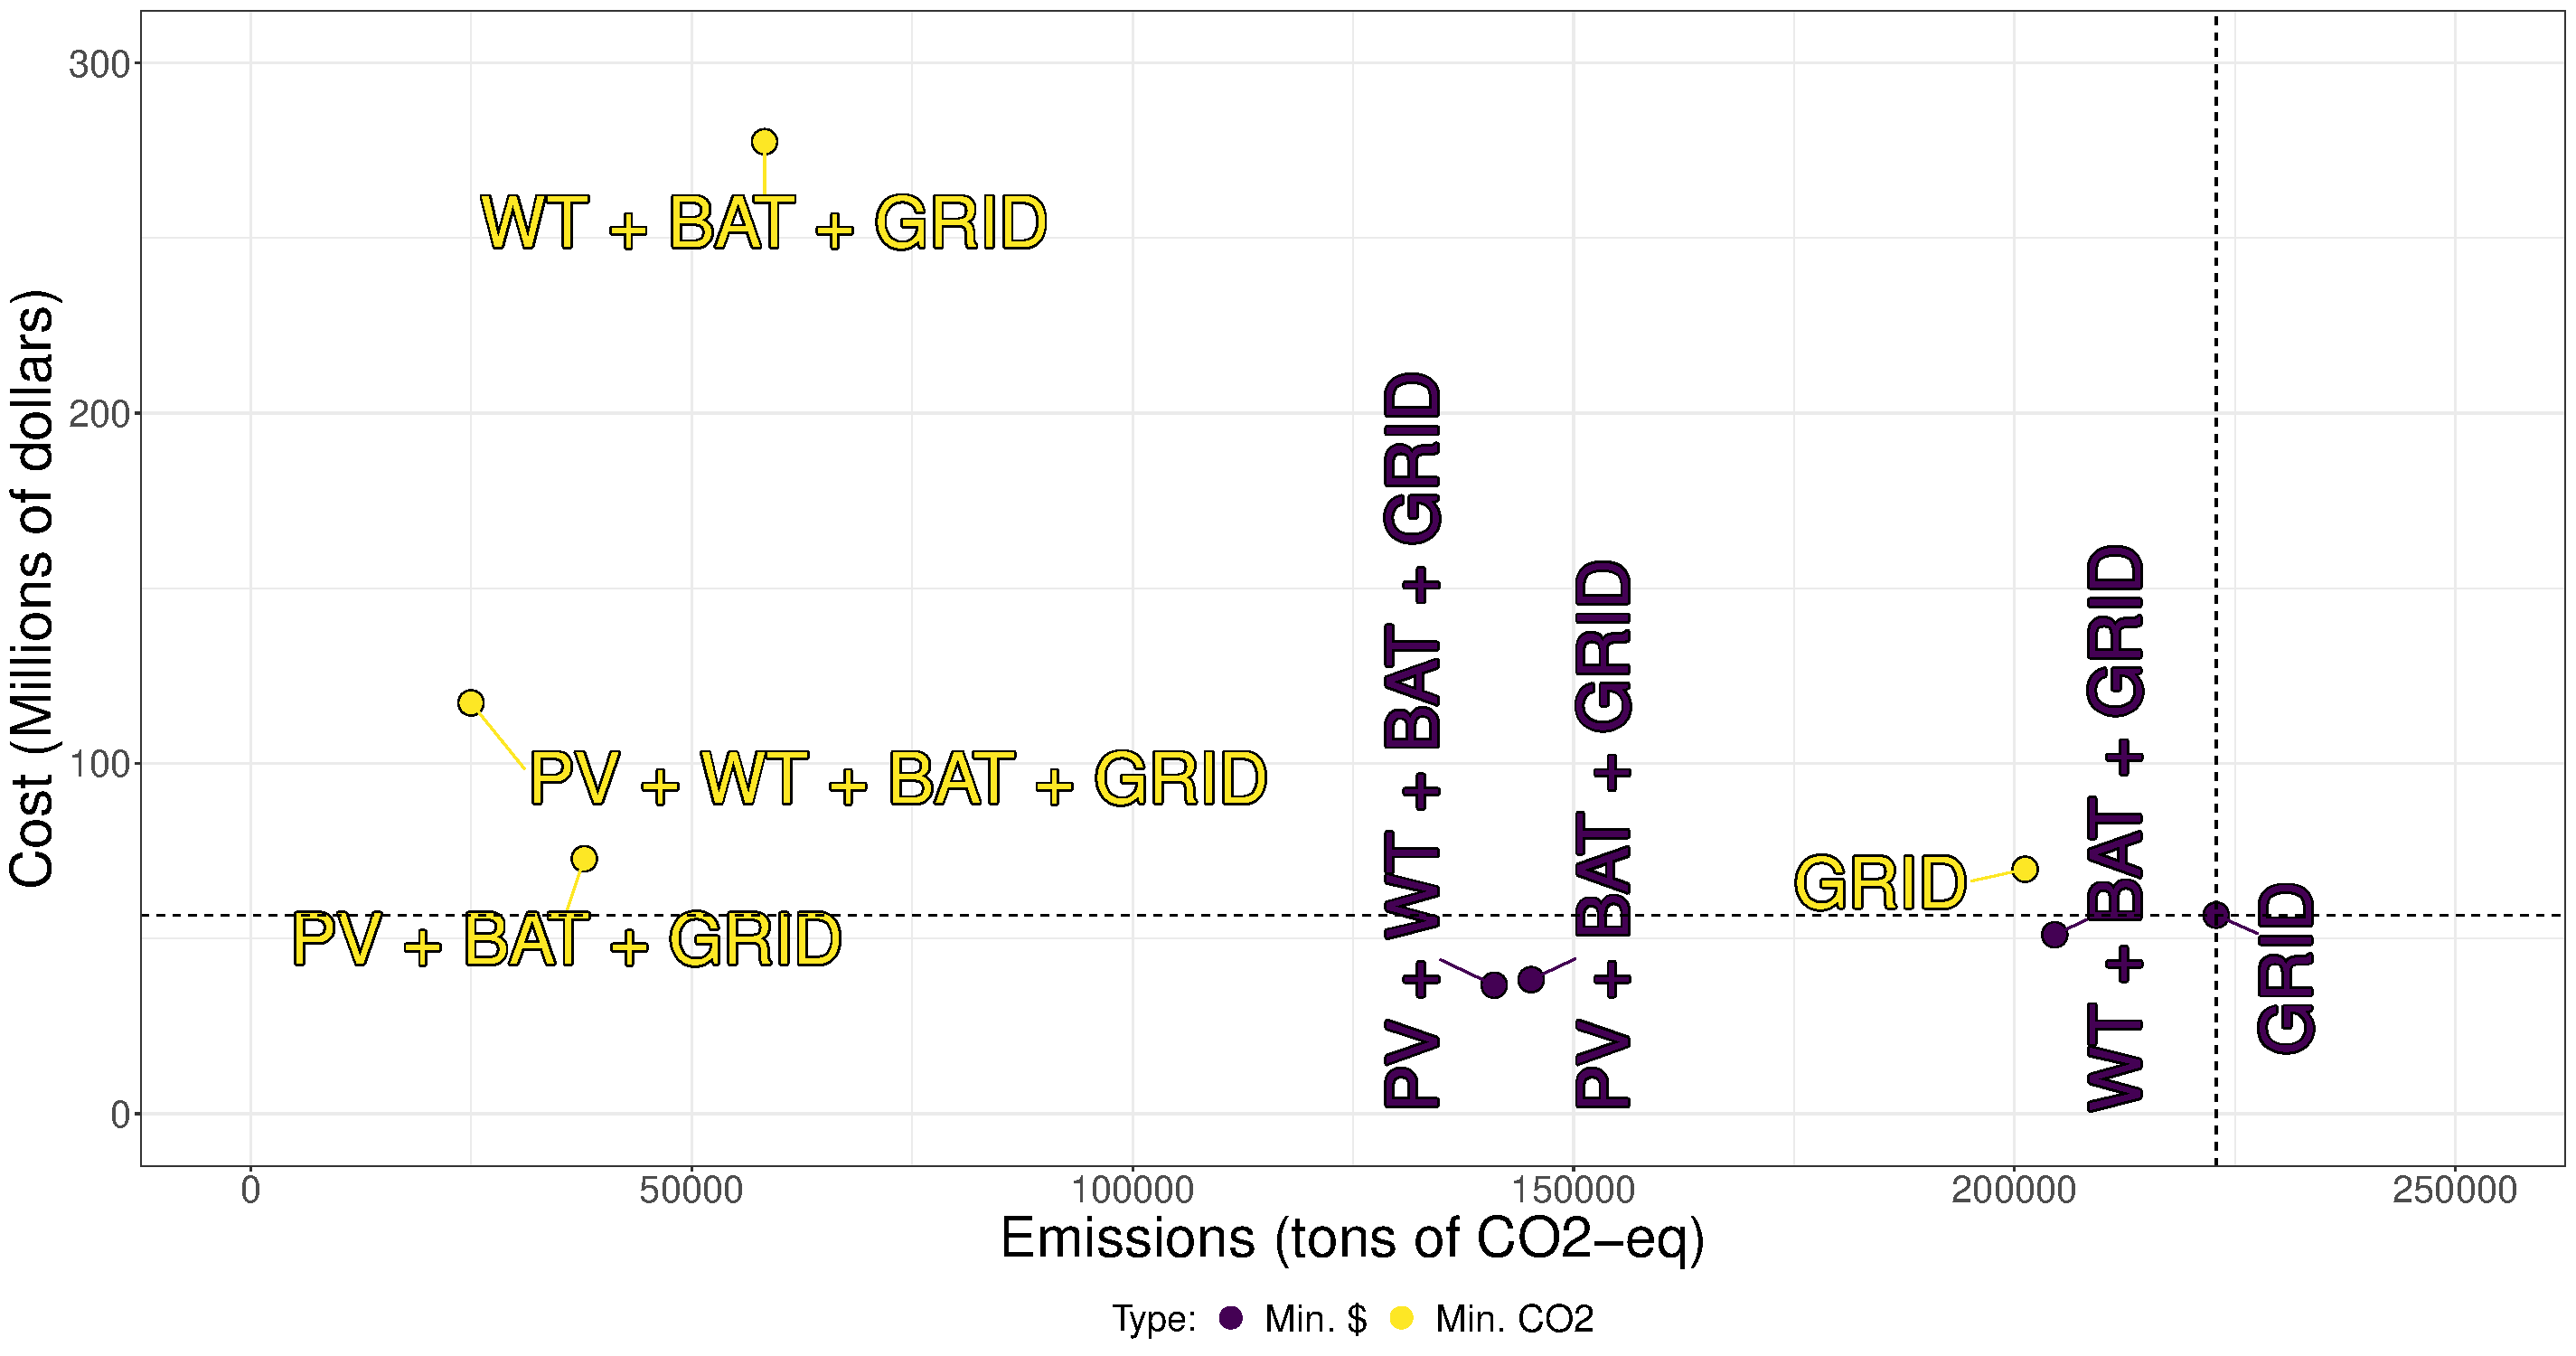
\includegraphics[width=.9\textwidth]{images/costs_vs_co2_scenarios_only_grid_costs.pdf}
  \caption{Costs vs \ch{CO2} emissions for the different scenarios.}
\end{figure}

\end{frame}
\addtocounter{framenumber}{-1}

\begin{frame}{Costs (\$) of reducing the environmental impact}


\begin{figure}[h]
\centering
  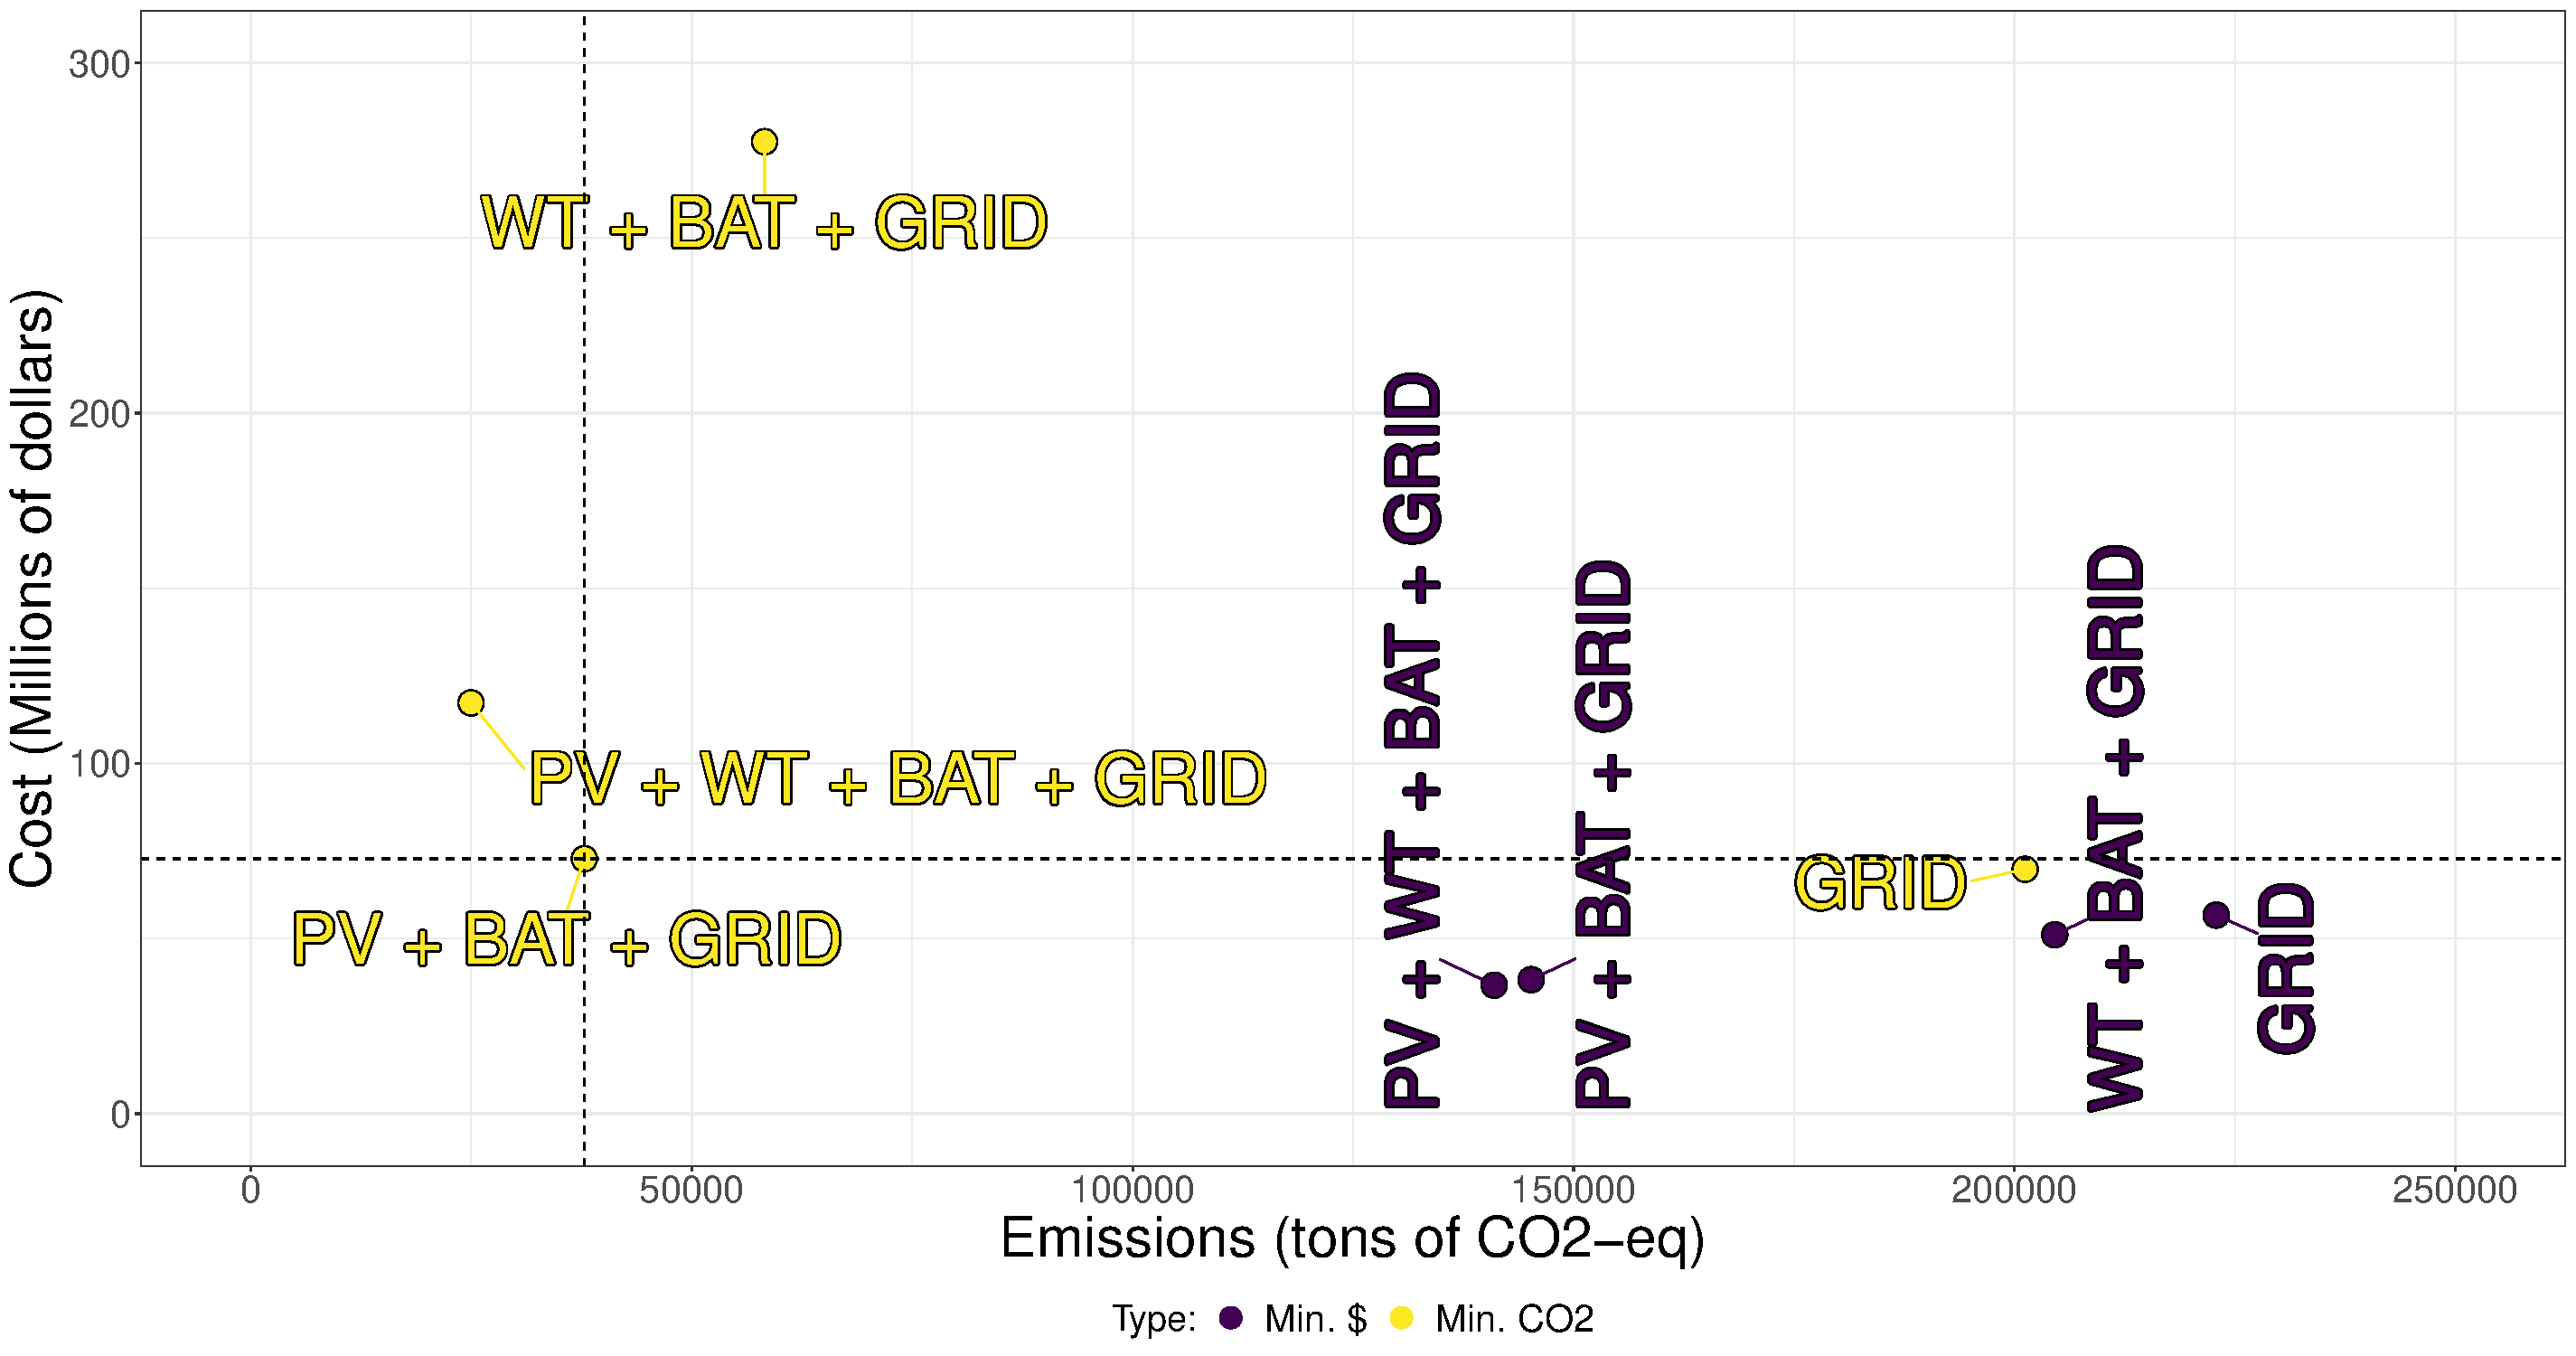
\includegraphics[width=.9\textwidth]{images/costs_vs_co2_scenarios_interesting_candidate.pdf}
  \caption{Costs vs \ch{CO2} emissions for the different scenarios.}
\end{figure}

\end{frame}


\begin{frame}{Sizing the IT part}
Defining the number of servers needed for the operation
\begin{itemize}
    \item Workload growth over time 
    \item New hardware generations that may be more power-efficient
    \item \textbf{\ch{CO2} from manufacturing the servers}      
\end{itemize}  

\ch{CO2}-eq computed based in the specifications of the integrated circuits~\footcite{gupta2022_ACT}  
\begin{itemize}
 \item Dell R740: 4020 vs 688 kg \ch{CO2}-eq
\end{itemize}
\end{frame}

\begin{frame}{Sizing the IT part}

\textbf{Is it worth to add/replace the servers every year?}
\begin{itemize}
 \item Decision made year by year (greedy approach)
 \item Optimal solution (all information is known in advance)
\end{itemize}
\textbf{Settings:}
\begin{itemize}
    \item Workload increase 25\% per year\footcite{cisco_global_cloud_index_2018}
    \item Server expected lifetime of 4 years
    \item 5 years of operation
\end{itemize}

\begin{table}[h]
  \small
  \label{tab:servers_specs} 
  \caption{Servers specifications for different generations.} \centering
  \begin{tabular}{|l|r|r|r|r|r|}
  \hline    
  \textbf{Year} & \textbf{CPU} &   \textbf{Cores} & \textbf{Pidle}  & \textbf{Pcore}  & \textbf{$\mathbf{kg\,\ch{CO2}\text{-}eq}$}  \\
  \hline
  < 2016      & Intel Xeon E5-2660 v2 & 20 & 52 & 7.5  & -   \\
  \hline
  2017, 2018 & Intel Xeon Platinum 8180 & 56 & 48.9 & 6.68  & 578.6   \\
  \hline
  2019, 2020   & AMD EPYC 7742  & 64 & 66.1 & 2.71  & 587.2 \\
  \hline
  2021        & AMD EPYC 7763 & 128 & 75.6 & 3     & 590.3 \\
  \hline
  
\end{tabular}  
\end{table}
\end{frame}


\begin{frame}{Sizing the IT part}
  \begin{center}
    \begin{figure}[h]    
      \centering
      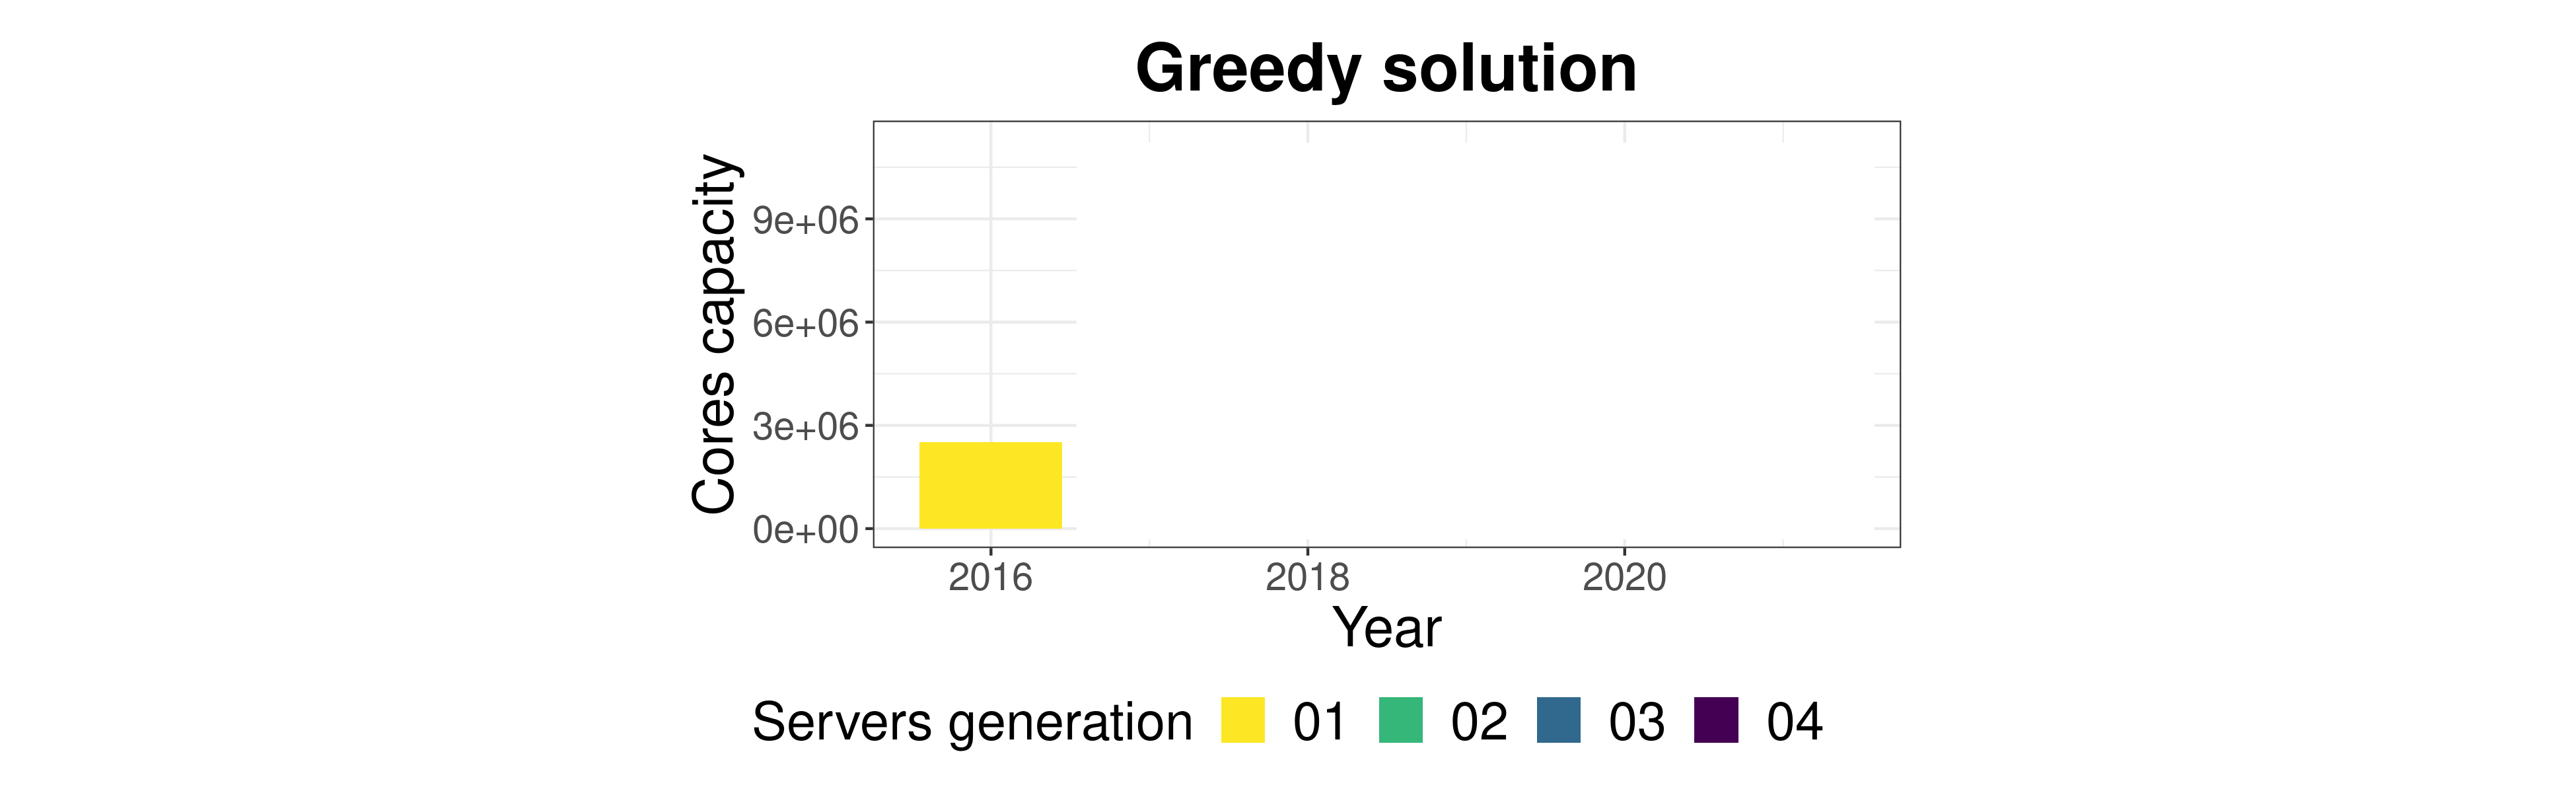
\includegraphics[width=.9\textwidth]{images/cloud_federation_evolution_lifetime_year1.png}
      \caption{Comparison between the optimal and greedy approaches.}
    \end{figure}    
  \end{center}  

  \begin{table}[h]
  \tiny
  \label{tab:servers_specs} 
  \caption{Servers specifications for different generations.} \centering
  \begin{tabular}{|l|l|r|r|r|r|r|}
  \hline    
  \textbf{Gen} & \textbf{Years} & \textbf{CPU} &   \textbf{Cores} & \textbf{Pidle}  & \textbf{Pcore}  & \textbf{$\mathbf{kg\,\ch{CO2}\text{-}eq}$}  \\
  \hline
  01      &  2016 < & Intel Xeon E5-2660 v2 & 20 & 52 & 7.5  & -   \\
  \hline
  02 & 2017, 2018 & Intel Xeon Platinum 8180 & 56 & 48.9 & 6.68  & 578.6   \\
  \hline
  03   & 2019, 2020 & AMD EPYC 7742  & 64 & 66.1 & 2.71  & 587.2 \\
  \hline
  04   & 2021      & AMD EPYC 7763 & 128 & 75.6 & 3     & 590.3 \\
  \hline
  
\end{tabular}  
\end{table}

\end{frame}

\addtocounter{framenumber}{-1}

\begin{frame}{Sizing the IT part}
  \begin{center}
    \begin{figure}[h]    
      \centering
      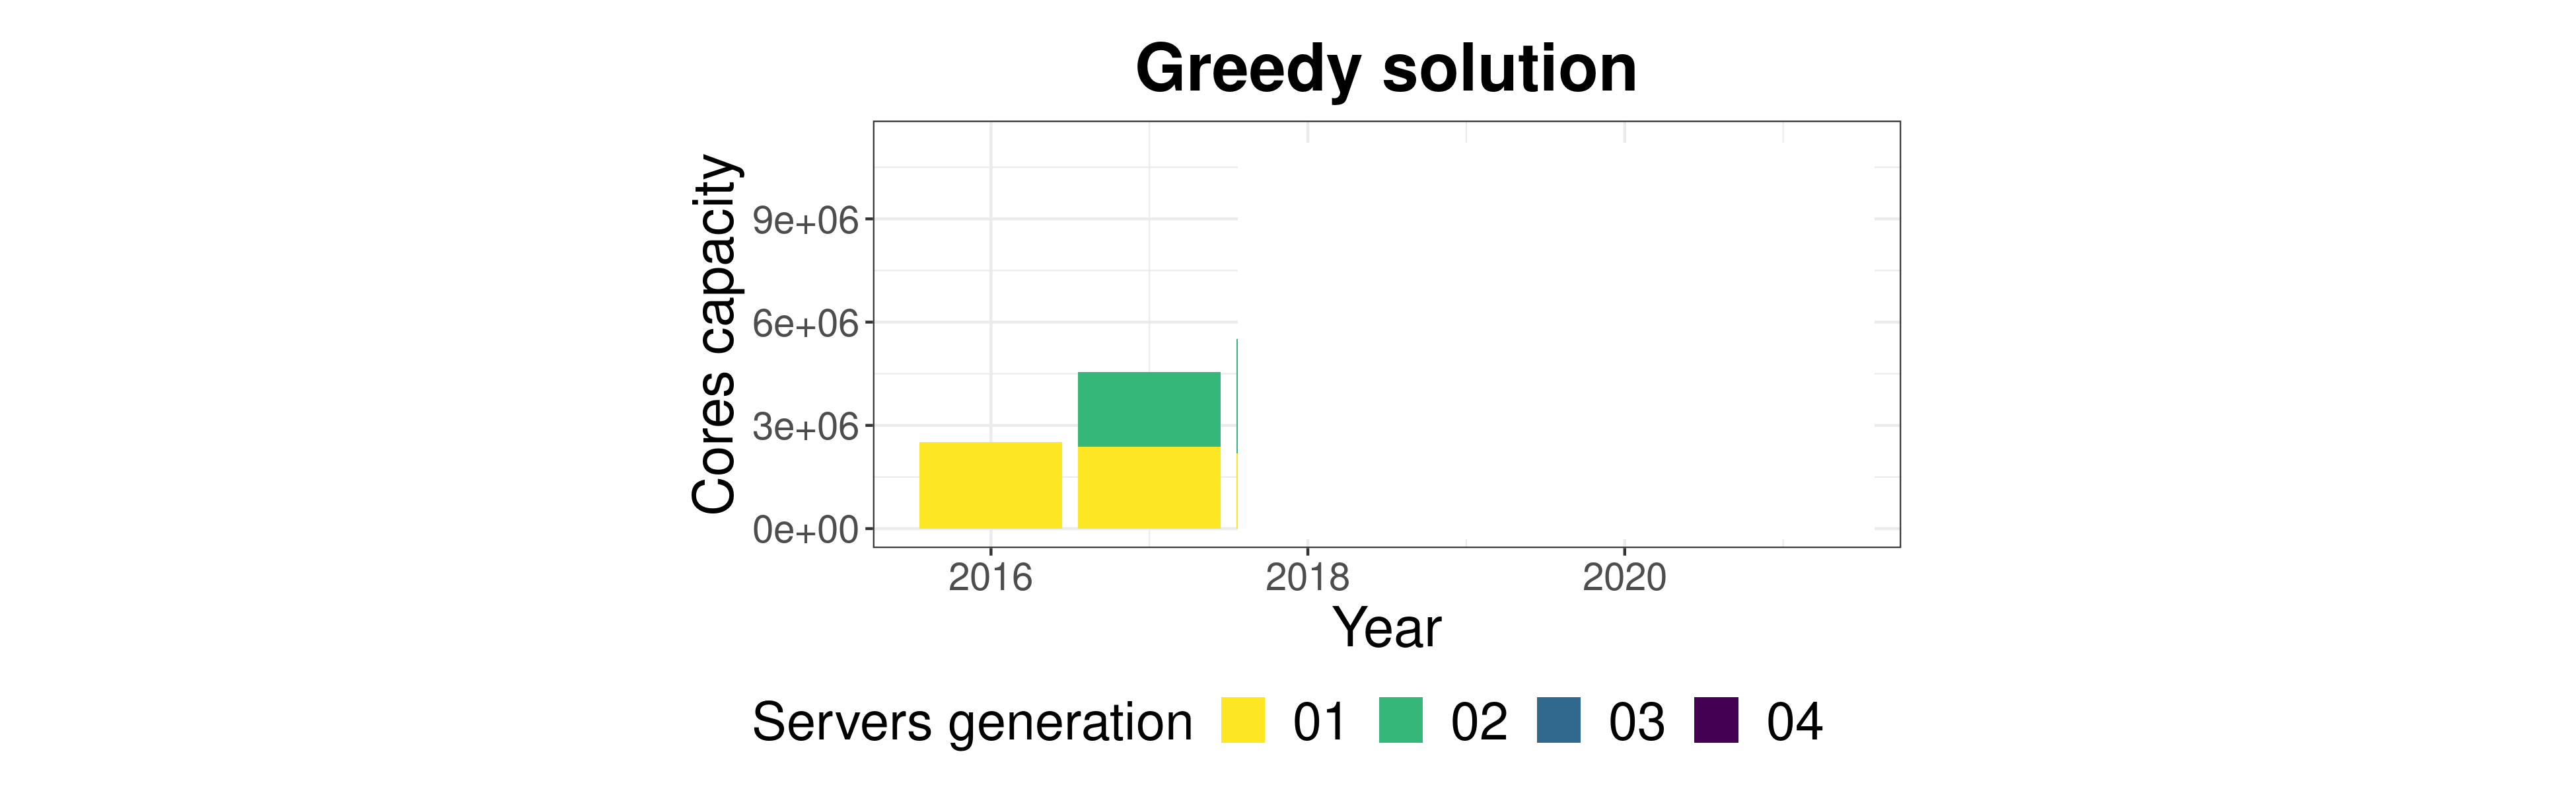
\includegraphics[width=.9\textwidth]{images/cloud_federation_evolution_lifetime_year2.png}
      \caption{Comparison between the optimal and greedy approaches.}
    \end{figure}    
  \end{center}  

  \begin{table}[h]
  \tiny
  \label{tab:servers_specs} 
  \caption{Servers specifications for different generations.} \centering
%  \vspace{-0.8cm}
  \begin{tabular}{|l|l|r|r|r|r|r|}
  \hline    
  \textbf{Gen} & \textbf{Years} & \textbf{CPU} &   \textbf{Cores} & \textbf{Pidle}  & \textbf{Pcore}  & \textbf{$\mathbf{kg\,\ch{CO2}\text{-}eq}$}  \\
  \hline
  01      &  2016 < & Intel Xeon E5-2660 v2 & 20 & 52 & 7.5  & -   \\
  \hline
  02 & 2017, 2018 & Intel Xeon Platinum 8180 & 56 & 48.9 & 6.68  & 578.6   \\
  \hline
  03   & 2019, 2020 & AMD EPYC 7742  & 64 & 66.1 & 2.71  & 587.2 \\
  \hline
  04   & 2021      & AMD EPYC 7763 & 128 & 75.6 & 3     & 590.3 \\
  \hline
  
\end{tabular}  
\end{table}

\end{frame}
\addtocounter{framenumber}{-1}
\begin{frame}{Sizing the IT part}
  \begin{center}
    \begin{figure}[h]    
      \centering
      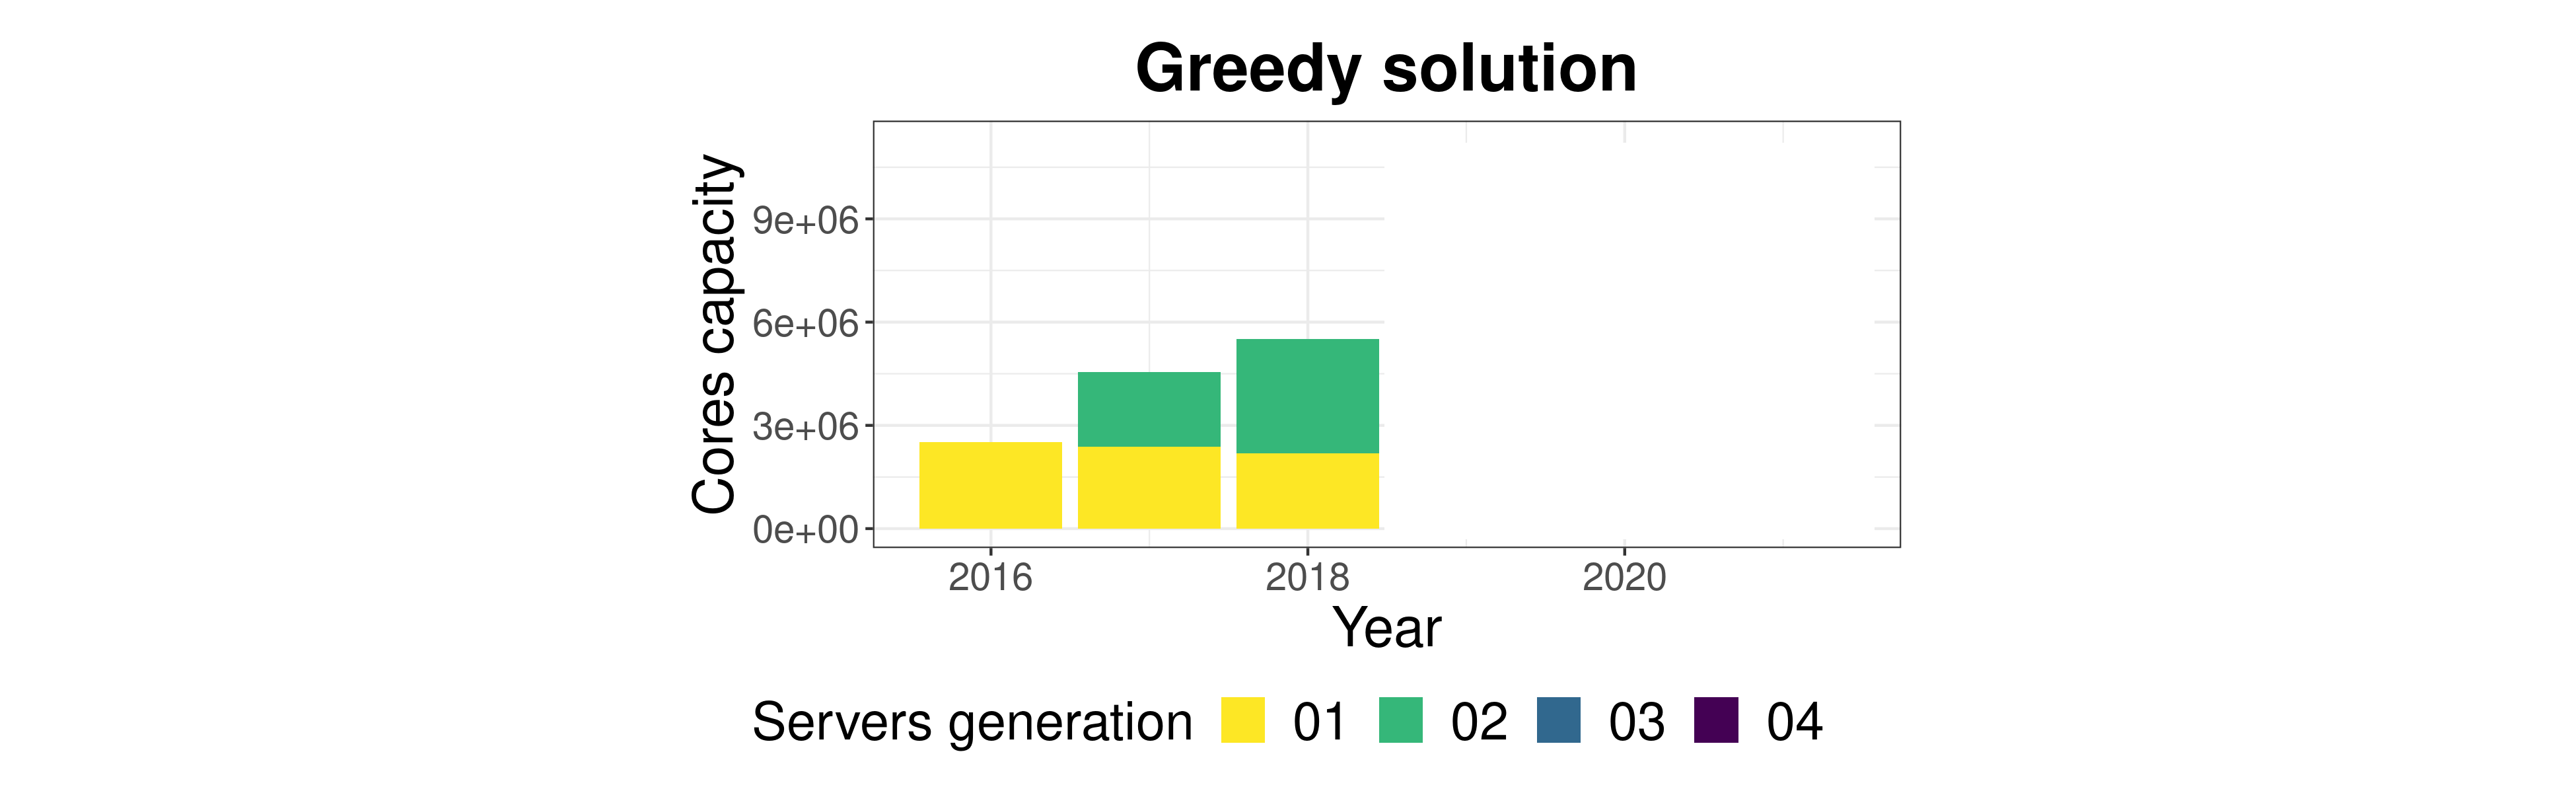
\includegraphics[width=.9\textwidth]{images/cloud_federation_evolution_lifetime_year3.png}
      \caption{Comparison between the optimal and greedy approaches.}
    \end{figure}    
  \end{center}  

  \begin{table}[h]
  \tiny
  \label{tab:servers_specs} 
  \caption{Servers specifications for different generations.} \centering
%  \vspace{-0.8cm}
  \begin{tabular}{|l|l|r|r|r|r|r|}
  \hline    
  \textbf{Gen} & \textbf{Years} & \textbf{CPU} &   \textbf{Cores} & \textbf{Pidle}  & \textbf{Pcore}  & \textbf{$\mathbf{kg\,\ch{CO2}\text{-}eq}$}  \\
  \hline
  01      &  2016 < & Intel Xeon E5-2660 v2 & 20 & 52 & 7.5  & -   \\
  \hline
  02 & 2017, 2018 & Intel Xeon Platinum 8180 & 56 & 48.9 & 6.68  & 578.6   \\
  \hline
  03   & 2019, 2020 & AMD EPYC 7742  & 64 & 66.1 & 2.71  & 587.2 \\
  \hline
  04   & 2021      & AMD EPYC 7763 & 128 & 75.6 & 3     & 590.3 \\
  \hline
  
\end{tabular}  
\end{table}

\end{frame}
\addtocounter{framenumber}{-1}
\begin{frame}{Sizing the IT part}
  \begin{center}
    \begin{figure}[h]    
      \centering
      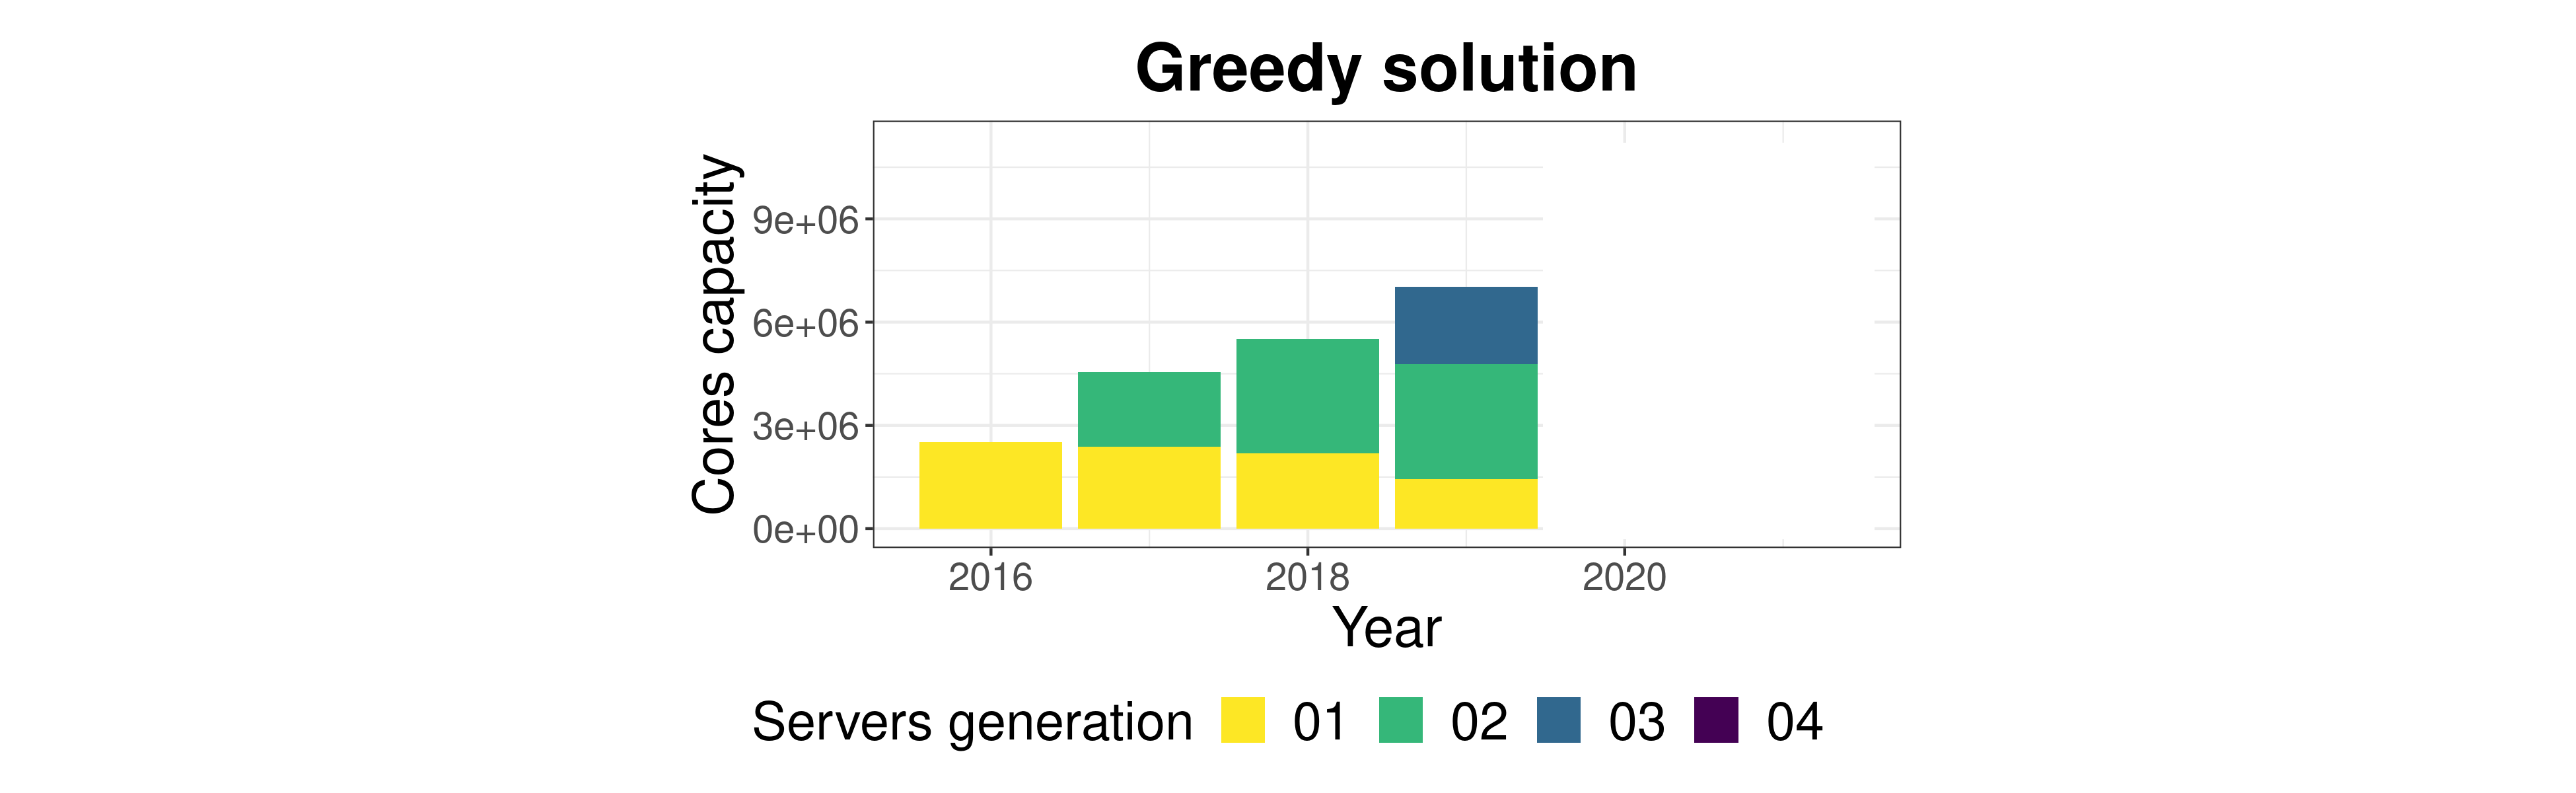
\includegraphics[width=.9\textwidth]{images/cloud_federation_evolution_lifetime_year4.png}
      \caption{Comparison between the optimal and greedy approaches.}
    \end{figure}    
  \end{center}  

  \begin{table}[h]
  \tiny
  \label{tab:servers_specs} 
  \caption{Servers specifications for different generations.} \centering
%  \vspace{-0.8cm}
  \begin{tabular}{|l|l|r|r|r|r|r|}
  \hline    
  \textbf{Gen} & \textbf{Years} & \textbf{CPU} &   \textbf{Cores} & \textbf{Pidle}  & \textbf{Pcore}  & \textbf{$\mathbf{kg\,\ch{CO2}\text{-}eq}$}  \\
  \hline
  01      &  2016 < & Intel Xeon E5-2660 v2 & 20 & 52 & 7.5  & -   \\
  \hline
  02 & 2017, 2018 & Intel Xeon Platinum 8180 & 56 & 48.9 & 6.68  & 578.6   \\
  \hline
  03   & 2019, 2020 & AMD EPYC 7742  & 64 & 66.1 & 2.71  & 587.2 \\
  \hline
  04   & 2021      & AMD EPYC 7763 & 128 & 75.6 & 3     & 590.3 \\
  \hline
  
\end{tabular}  
\end{table}

\end{frame}
\addtocounter{framenumber}{-1}
\begin{frame}{Sizing the IT part}
  \begin{center}
    \begin{figure}[h]    
      \centering
      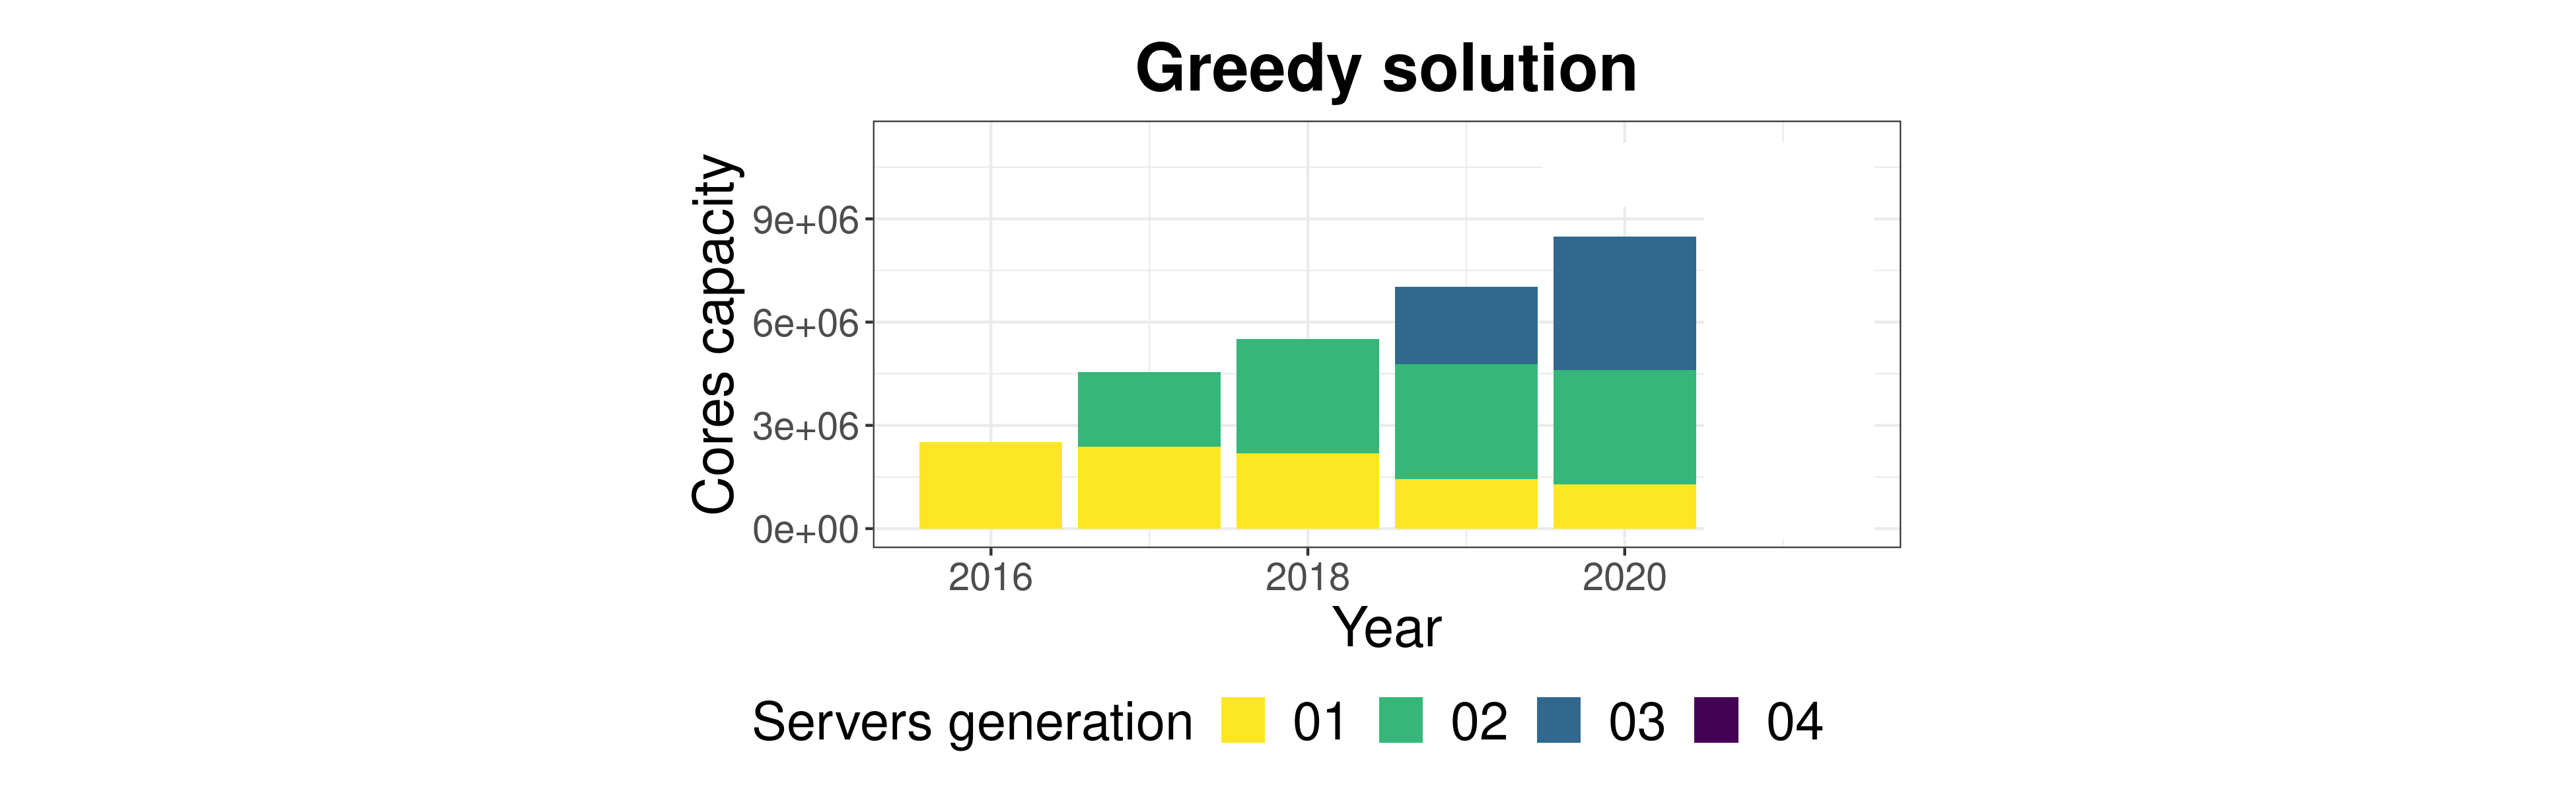
\includegraphics[width=.9\textwidth]{images/cloud_federation_evolution_lifetime_year5.png}
      \caption{Comparison between the optimal and greedy approaches.}
    \end{figure}    
  \end{center}  

  \begin{table}[h]
  \tiny
  \label{tab:servers_specs} 
  \caption{Servers specifications for different generations.} \centering
%  \vspace{-0.8cm}
  \begin{tabular}{|l|l|r|r|r|r|r|}
  \hline    
  \textbf{Gen} & \textbf{Years} & \textbf{CPU} &   \textbf{Cores} & \textbf{Pidle}  & \textbf{Pcore}  & \textbf{$\mathbf{kg\,\ch{CO2}\text{-}eq}$}  \\
  \hline
  01      &  2016 < & Intel Xeon E5-2660 v2 & 20 & 52 & 7.5  & -   \\
  \hline
  02 & 2017, 2018 & Intel Xeon Platinum 8180 & 56 & 48.9 & 6.68  & 578.6   \\
  \hline
  03   & 2019, 2020 & AMD EPYC 7742  & 64 & 66.1 & 2.71  & 587.2 \\
  \hline
  04   & 2021      & AMD EPYC 7763 & 128 & 75.6 & 3     & 590.3 \\
  \hline
  
\end{tabular}  
\end{table}

\end{frame}
\addtocounter{framenumber}{-1}
\begin{frame}{Sizing the IT part}
  \begin{center}
    \begin{figure}[h]    
      \centering
      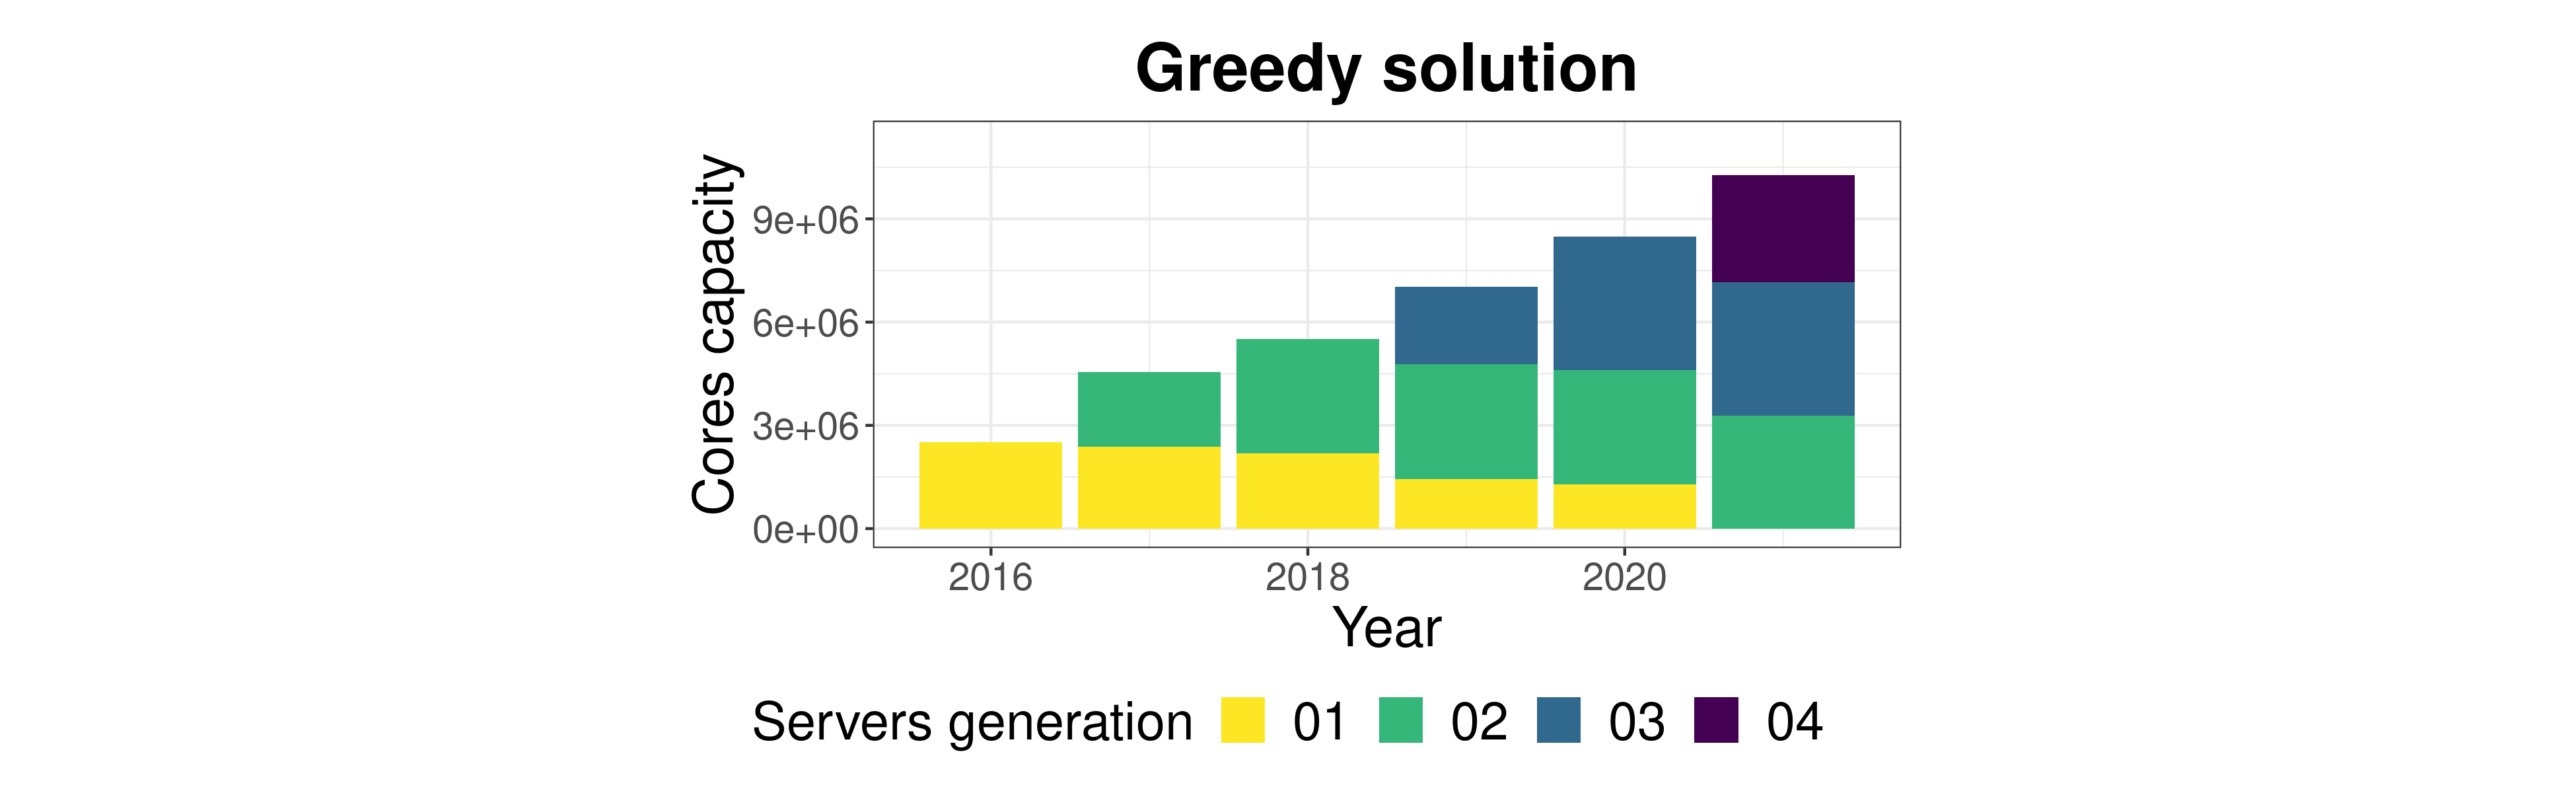
\includegraphics[width=.9\textwidth]{images/cloud_federation_evolution_lifetime_year6.png}
      \caption{Comparison between the optimal and greedy approaches.}
    \end{figure}    
  \end{center}  

  \begin{table}[h]
  \tiny
  \label{tab:servers_specs} 
  \caption{Servers specifications for different generations.} \centering
%  \vspace{-0.8cm}
  \begin{tabular}{|l|l|r|r|r|r|r|}
  \hline    
  \textbf{Gen} & \textbf{Years} & \textbf{CPU} &   \textbf{Cores} & \textbf{Pidle}  & \textbf{Pcore}  & \textbf{$\mathbf{kg\,\ch{CO2}\text{-}eq}$}  \\
  \hline
  01      &  2016 < & Intel Xeon E5-2660 v2 & 20 & 52 & 7.5  & -   \\
  \hline
  02 & 2017, 2018 & Intel Xeon Platinum 8180 & 56 & 48.9 & 6.68  & 578.6   \\
  \hline
  03   & 2019, 2020 & AMD EPYC 7742  & 64 & 66.1 & 2.71  & 587.2 \\
  \hline
  04   & 2021      & AMD EPYC 7763 & 128 & 75.6 & 3     & 590.3 \\
  \hline
  
\end{tabular}  
\end{table}

\end{frame}
\addtocounter{framenumber}{-1}
\begin{frame}{Sizing the IT part}
  The optimal solution emits 13.4\% less \ch{CO2}.
  \begin{center}
    \begin{figure}[h]    
      \centering
      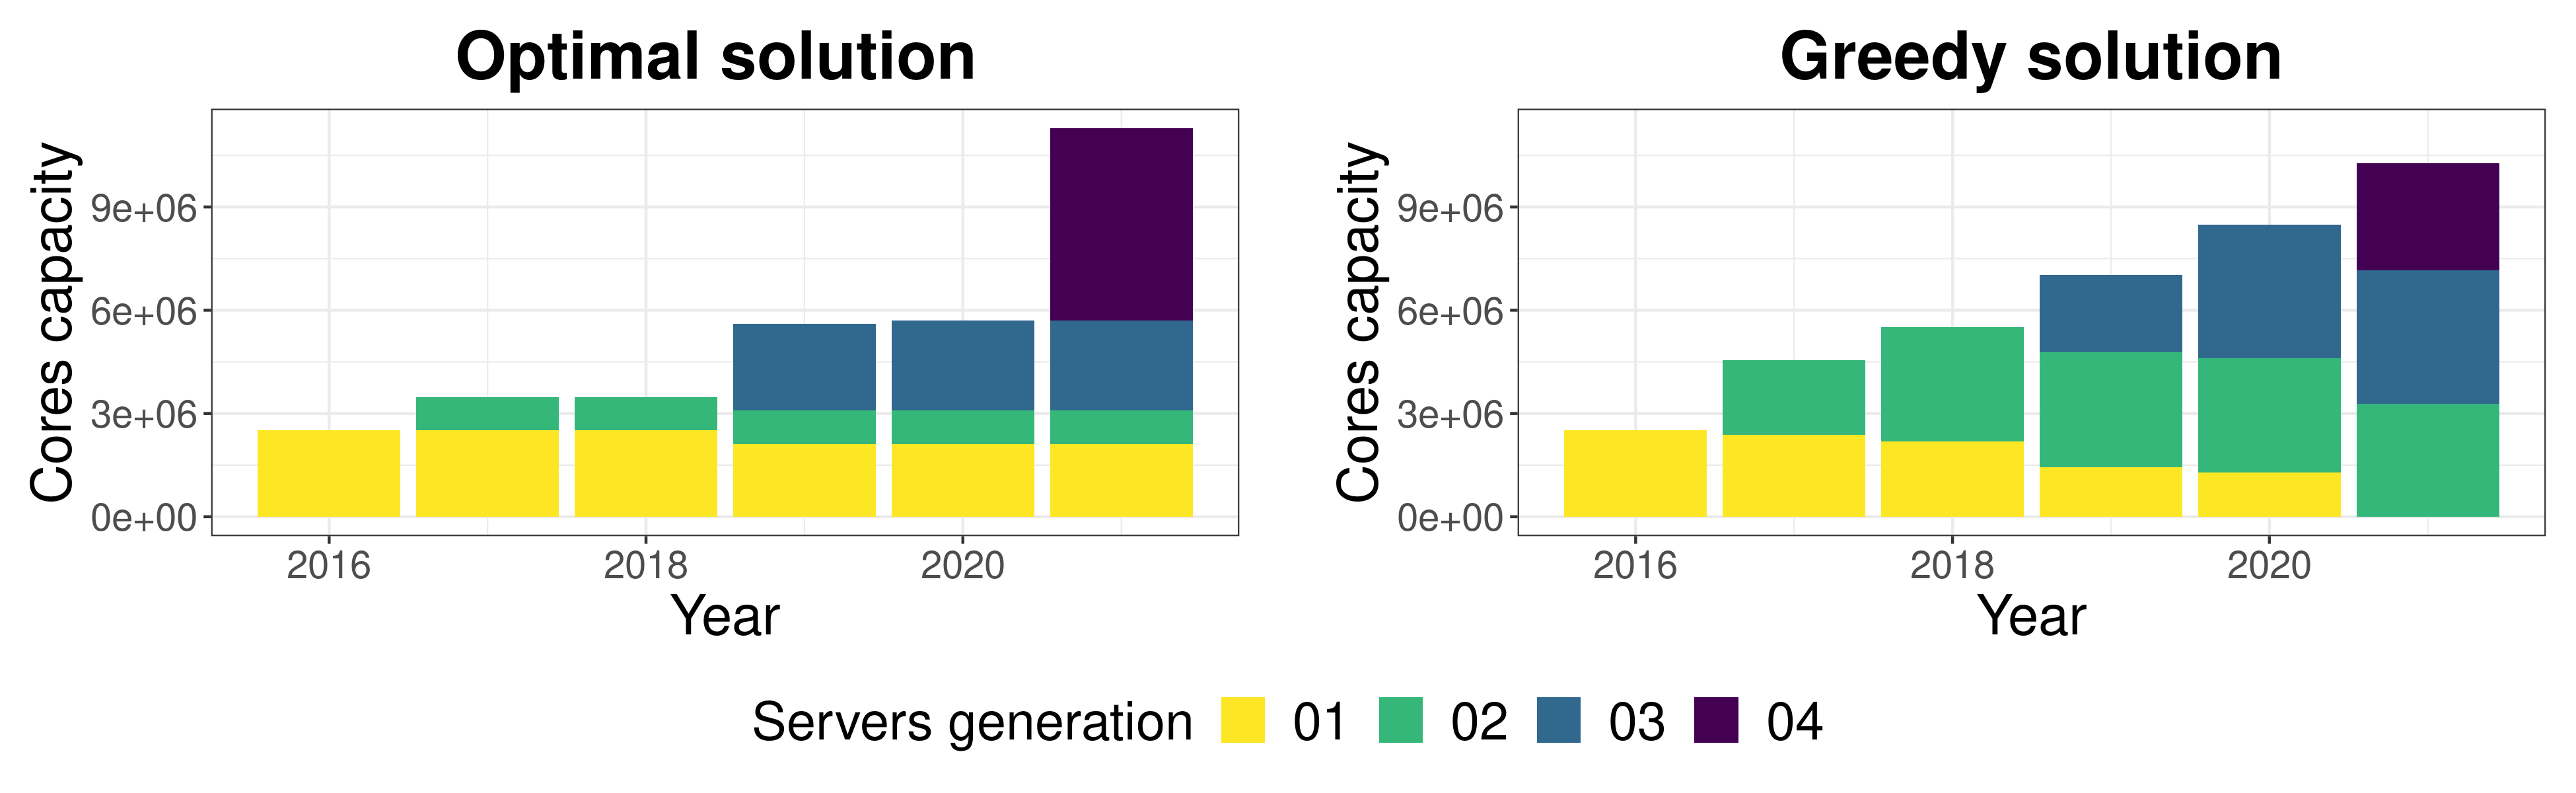
\includegraphics[width=.9\textwidth]{images/cloud_federation_evolution_lifetime.png}
      \caption{Comparison between the optimal and greedy approaches.}
    \end{figure}    
  \end{center}  

  \begin{table}[h]
  \tiny
  \label{tab:servers_specs} 
  \caption{Servers specifications for different generations.} \centering
%  \vspace{-0.8cm}
  \begin{tabular}{|l|l|r|r|r|r|r|}
  \hline    
  \textbf{Gen} & \textbf{Years} & \textbf{CPU} &   \textbf{Cores} & \textbf{Pidle}  & \textbf{Pcore}  & \textbf{$\mathbf{kg\,\ch{CO2}\text{-}eq}$}  \\
  \hline
  01      &  2016 < & Intel Xeon E5-2660 v2 & 20 & 52 & 7.5  & -   \\
  \hline
  02 & 2017, 2018 & Intel Xeon Platinum 8180 & 56 & 48.9 & 6.68  & 578.6   \\
  \hline
  03   & 2019, 2020 & AMD EPYC 7742  & 64 & 66.1 & 2.71  & 587.2 \\
  \hline
  04   & 2021      & AMD EPYC 7763 & 128 & 75.6 & 3     & 590.3 \\
  \hline
  
\end{tabular}  
\end{table}

\end{frame}

\begin{frame}{Summary - second main contribution}

  \begin{itemize}    
  \item Linear program formulation for \textbf{sizing} and \textbf{operating} DCs 
  \begin{itemize}    
    \item renewable and IT infrastructure
  \end{itemize}    

  \item Characteristics of each region   
  \begin{itemize}    
    \item climate conditions, energy mix
  \end{itemize}    
  \item Follow-the-renewables
  \item Flexible to evaluate many scenarios
  \item Solved in polynomial time  
  \end{itemize}    
\end{frame}

\begin{frame}{Future research directions}
  \begin{itemize}
  \item Other types of environmental impact      
  \item Migrating the workload  
  \item Robustness  
  \item Degradation of the infrastructure over the years
  \item Sizing new data centers (renewable and IT infrastructure)  
  \end{itemize}     
\end{frame}

\begin{frame}{Acknowledgments}
  \begin{itemize}
  \item LabEx PERSYVAL-Lab (``ANR-11-LABX-0025-01'')
  \item São Paulo Research Foundation (FAPESP) grants 2021/06867-2 and 2019/26702-8.
   \item EuroHPC EU Regale project (g.a. 956560)
   \item INCT of the Future Internet for Smart Cities funded by CNPq proc. 465446/2014-0, Coordenação de Aperfeiçoamento de Pessoal de Nível Superior – Brasil (CAPES) – Finance Code 001, FAPESP proc. 14/50937-1, and FAPESP proc. 15/24485-9
  \end{itemize}     
\end{frame}


\begin{frame}{Thank you !}


\textbf{Thank you for your attention!}\\
Contact: miguel.felipesilva@gmail.com


\par\noindent\rule{\textwidth}{0.5pt}


\begin{center}


\textbf{Strategies for operating and sizing low-carbon cloud data centers}

Miguel Felipe Silva Vasconcelos

Advisors: Fanny Dufossé and Daniel Cordeiro\\

Université Grenoble Alpes, Grenoble, France \\
Universidade de São Paulo, Brazil

\end{center}

\end{frame}

\appendix


\begin{frame}[allowframebreaks]  
  \printbibliography
\end{frame}

\begin{frame}{Baselines}

  \alert{\textbf{WSNB}} (\textbf{W}orkload \textbf{s}hifting
  \textbf{n}on \textbf{b}rownout)\footfullcite{XU2020191}:

  \begin{itemize}
  \item Allocates the workload to the nearest DC that has available green power
  \item Follow-the-renewables strategy applied for the initial
    allocation
  \item Does not perform live-migrations
  \item Does not shutdown under-utilized servers
  \end{itemize}  
  
\end{frame}





\begin{frame}{Baselines}

  \alert{\textbf{FollowME@Source}}\footfullcite{ALI2021110907}:

  \begin{itemize}
  \item Allocation step: tries to allocate the incoming VMs to the
    greenest DC

  \item Migration step: Either only intra (origin = destination) or
    inter (origin != destination) DC

    \begin{itemize}
    \item Intra DC: executed at each DC separately
    \item Inter DC: tries to migrate the workload to the greenest DC
    \end{itemize}       
  \item Under-utilized servers are shut down (server consolidation)
  \item Do not consider network for migration planning

  \end{itemize}    
\end{frame}


\begin{frame}{Baselines}
  \textbf{Follow-the-renewables strategy}
  \begin{itemize}
  \item Only for the VM allocation
    \begin{itemize}
    \item WSNB and FollowME@S Intra
    \end{itemize}  
  \item During the whole execution of the workload
    \begin{itemize}
    \item NEMESIS, c-NEMESIS and FollowME@S Inter
    \end{itemize}  
  \end{itemize}    
\end{frame}


\begin{frame}{Impact of adding wind turbines (WT) }



  \begin{itemize}    
     \item  Can further reduce 34\% the carbon emissions in comparison to only using PVs and batteries.
     \item However, requires larger land area (1 to 3 WT per km²)
  \end{itemize}
  \begin{table}[h]
  \caption{Computed number of WT for each location.}\label{tab:results_wt} \centering
  \begin{tabular}{|l|r|}
  \hline
    
  \textbf{Location} &   \textbf{Number of WT} \\
  \hline
  Johannesburg & 59   \\
  \hline
  Pune         & 26 \\
  \hline
  Canberra    & 67 \\
  \hline
  Dubai       &  79  \\
  \hline
  Singapore   & 37 \\
  \hline     
  Seoul       & 109  \\
  \hline
  Virginia   & 39 \\
  \hline
  São Paulo   & 87 \\
  \hline 
  Paris    &   22 \\
  \hline
  
\end{tabular}  
\end{table}

\end{frame}

\begin{frame}{Impact of adding wind turbines (WT) }
    

  \begin{itemize}    
     \item  Can further reduce 34\% the carbon emissions in comparison to only using PVs and batteries.
     \item However, requires larger land area (1 to 3 WT per km²)
  \end{itemize}
\begin{table}[H]
  
  \caption{Capacity Factor (in \%) for solar panels and wind turbines at each location.}\label{tab:capacity_factor} \centering
  
  \begin{tabular}{|l|r|r|}
  \hline    
  \textbf{Location} &   \textbf{PV} & \textbf{WT}  \\
  \hline
  Johannesburg & 25.55 & 12.96  \\
  \hline
  Pune        &  24.26   & 10.04    \\
  \hline
  Canberra    & 22.08    & 12.97  \\
  \hline
  Dubai      & 25.28      & 13.98   \\
  \hline
  Singapore & 17.68    & 8.58   \\
  \hline     
  Seoul      & 18.81   &  9.41   \\
  \hline
  Virginia   & 19.83   &  14.68 \\
  \hline
  São Paulo  & 21.74   &  10.06    \\
  \hline 
  Paris      & 15.37   &  23.51   \\
  \hline  

\end{tabular}
\end{table}
  
\end{frame}

\begin{frame}{Wasted energy}  
  \begin{table}[!ht]

    \caption{Wasted energy in the migrations (Wh) for the Azure workload.}\label{tab:wasted_mig} \centering
    \begin{tabular}{|l|r|r|}
      \hline
      \textbf{Algorithm}  & \textbf{Origin} & \textbf{Target}   \\
      \hline
      NEMESIS   & 539.6  & 491.1 \\
      \hline
      c-NEMESIS &  39.3 & 24.1  \\
      \hline
      FollowMe@S Intra & 163 128.1  & 93 298.9  \\
      \hline
      FollowMe@S Inter & 175 086.3  & 105 528.8 \\
      \hline
    \end{tabular}
  \end{table} 
\end{frame}

\begin{frame}{Flexibility in the scheduling}
  
  What is the impact in carbon emissions of delaying $\alpha$ percent of the jobs up to $\beta$ time slots (1h per time slot) ?
 % \pause

  \begin{table}[h]
\caption{Reductions in total carbon emissions ( \% ) in comparison to the scenario where it is not possible to delay the workload. }\centering
\label{tab:flex_scheduling}
\begin{tabular}{|l|r|r|r|r|r|r|r|r|r|}
  \hline
  \small
\backslashbox{$\alpha$}{$\beta$} &   \textcolor{black}{\textbf{ 1}} &  \textcolor{black}{\textbf{ 24 }} &  \textcolor{black}{\textbf{ 48 }}  &   \textcolor{black}{\textbf{ 72 }} &   \textcolor{black}{\textbf{ 96 }} &   \textcolor{black}{\textbf{ 120  }} &   \textcolor{black}{\textbf{ 144 }} &   \textcolor{black}{\textbf{ 168 }} \\ 
     \hline
 \textcolor{black}{ \textbf{10}}   &  0.46  &  3.14 &  3.48 &  3.66 &  3.76 &  3.81 &  3.85 &  3.85 \\ 
\hline
 \textcolor{black}{ \textbf{20}}   &  0.84  &  3.85 &  4.11 &  4.21 &  4.21 &  4.21 &  4.22 &  4.22 \\ 
\hline
 \textcolor{black}{ \textbf{30}}   &  1.15  &  4.07 &  4.25 &  4.25 &  4.26 &  4.26 &  4.27 &  4.27 \\ 
\hline
 \textcolor{black}{ \textbf{40}}   &  1.42  &  4.15 &  4.25 &  4.26 &  4.27 &  4.28 &  4.28 &  4.29 \\ 
\hline
 \textcolor{black}{ \textbf{50}}   &  1.65  &  4.22 &  4.26 &  4.27 &  4.28 &  4.29 &  4.3 &  4.3 \\ 
\hline
\end{tabular}
\end{table}

\end{frame}




\begin{frame}{Network congestion}  
  
  \begin{table}[!ht]
    \small	
    \caption{Extra seconds during migrations compared to the case when
      there is no congestion for the Azure workload, where  ``avg.'' stands for the average of the observations, ``max.'' for the maximum value, and ``rel.'' for the relative value.} \label{ tab:wasted_seconds } \centering
    \begin{tabular}{|l|r|r|r|}
      \hline      
      \textbf{Algorithm}  & \textbf{avg. rel.} &  \textbf{max. rel.} &
                                                                       \textbf{Total
                                                                       extra
                                                                       seconds}
      \\
      \hline
      NEMESIS   & 1.6 & 3.98  & 86 235.5 \\
      \hline
      c-NEMESIS & 1.0 & 1.32  & 4 224.4\\
      \hline      
      FollowME@S Intra & 4.4 & 25.56  & 16 384 188.8  \\
      \hline      
      FollowME@S Inter & 7.8 & 157.24  & 18 531 893.3 \\      
      \hline

    \end{tabular}
  \end{table}
  \normalsize  
\end{frame}

\begin{frame}{Input: DCs irradiation used in second part}
      \begin{center}
        \begin{figure}[!h]
          \centering
          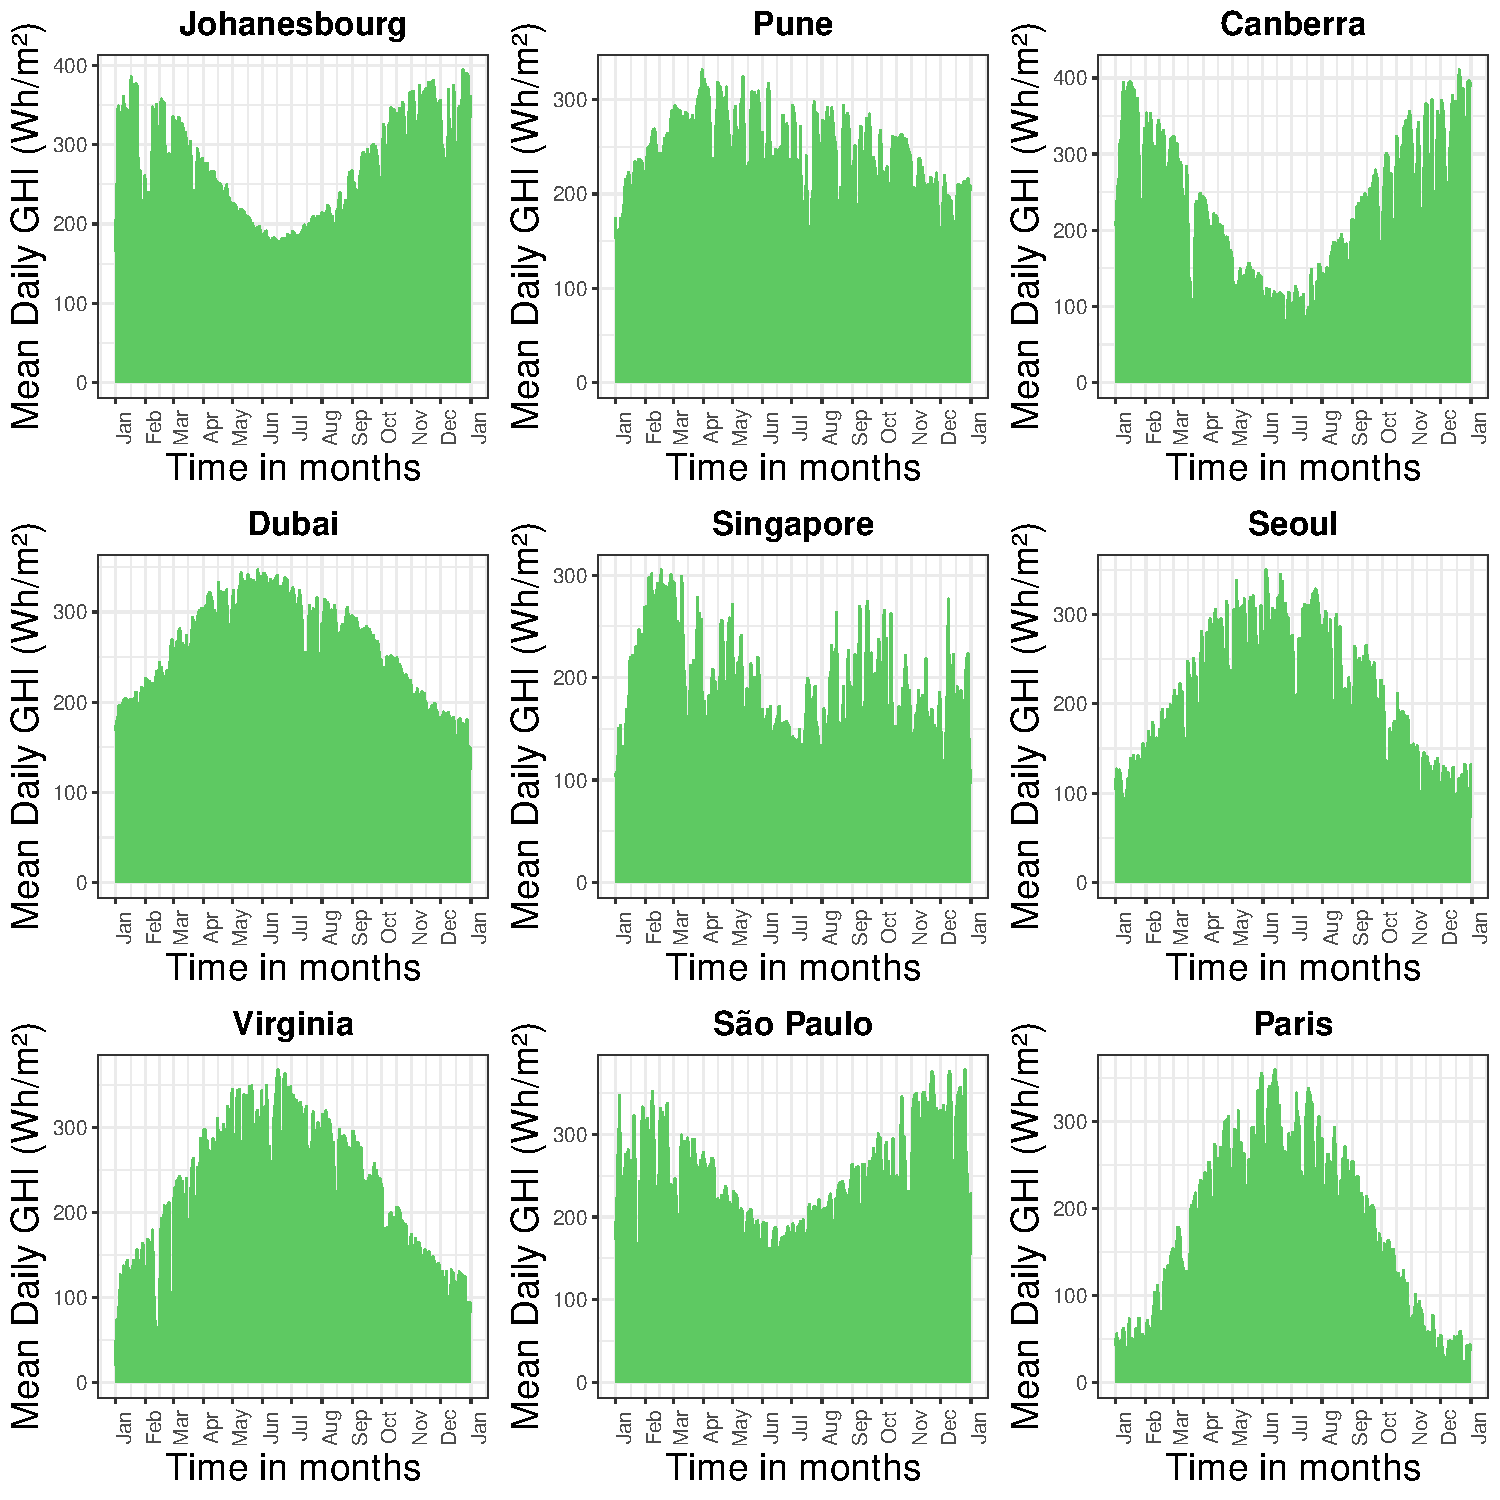
\includegraphics[width=.5\textwidth]{images/pv_ghi.pdf}
          \caption{Solar Irradiation at different locations in
            2021. Source: NASA's MERRA-2.}
        \end{figure}
      \end{center}
\end{frame}


\begin{frame}{Performance of the migration planning algorithm}

      \begin{itemize}          
          \item Will all the network links be evaluated all the time?
          \item No. Using the "migration history" reduces the search space
          \item Planning is made between servers, if server a server already has a migration planed, it will not be evaluated anymore
          
      \end{itemize}
\end{frame}


\begin{frame}{What if my workload require ms to be scheduled?}
      \begin{itemize}                    
          \item Allocation and migration steps could be executed in parallel
          \item Precomputations
          \item Azure uses parallel instances of the scheduler service, and cache mechanisms \footfullcite{protean}  \end{itemize}
\end{frame}




\begin{frame}{DCs all over the world for c-NEMESIS}
    \begin{itemize}    
        \item Multiple instances (for availability reasons, taking into account the energy consumption)
        \item 1 global controller
        \item N-regional controllers (Azure uses 1 instance to manage 10-100k machines)\footfullcite{protean}
        \item Response-time and Quality-of-Service
        \begin{itemize}            
        \item Select DCs with acceptable latency
        \item If workload is too restrictive: no migration
        \end{itemize}        
    \end{itemize}
\end{frame}

\begin{frame}{Changes or Failure in the network}
    \begin{itemize}
        \item Cloud platforms have detection systems for failure or changes in the network
        \item Information can be incorporated to the controller
    \end{itemize}
\end{frame}


\begin{frame}{Incorporating other sources of environmental impact}
    
    \begin{itemize}    
        
        \item Multi-objective optimization
        \item Evaluate the trade-offs of optimizing one type of environmental impact regarding the others        

    \end{itemize}            

\end{frame}


\begin{frame}{Heterogeneous servers in c-NEMESIS}

    \begin{itemize}    
    
        \item Algorithm is agnostic to servers specification
        \item Different clusters with homogeneous servers
        \item Considered workload will execute for a fixed amount of time
        \item Does not invalidate the analysis of the impact in the network

    \end{itemize}        

\end{frame}


\begin{frame}{Adopting the solutions}
    \begin{itemize}        
        \item All software is open source, documented, and reproducible
        \item Feedback from industry can help improve the assumptions
    \end{itemize}        
\end{frame}

\begin{frame}{Duration of time slots}
    \begin{itemize}
        \item MERRA-2 provide solar irradiation data as Short-wave irradiation (Wh/m2)            
        \item Tested with shorter duration (5 min), small differences in the sizing 
        \item Long-term sizing: changes between seasons (winter and summer) have higher impact
    \end{itemize}
\end{frame}


\begin{frame}{How to model migrations in the LP ?}
\begin{itemize}        
    \item Possible modeling:    
    \item Classify the workload into groups (regarding their response time requirements): 
    \item workload of group 1 = can only be executed in DCs A and B 
    \item workload of group 2 = can only be executed in DCs B and C
    
\end{itemize}
\end{frame}



\begin{frame}{Why LP ?}
\begin{itemize}    
    \item Using only linear variables allow for finding polynomial time solution:
    \begin{itemize}
        \item $\approx$ 2 min for 1 year sizing (pv + bat + grid)
        \item $\approx$ 40 min for 5 year sizing (IT sizing)
        \item Important to compare multiple scenarios
    \end{itemize}    
    \item Most studies in the literature uses MILP
    \item Other example of strategies: iterative methods as Genetic Algorithms
\end{itemize}
\end{frame}

\begin{frame}{Rebound effect}
\begin{itemize}    
    \item Clouds will become low-carbon, will the usage increase ? 
    \item Workloads keep increasing
    \item What really needs to be computed?
    \item Integration with social sciences, how to reeducate the users ?   
\end{itemize}
\end{frame}


\begin{frame}{Decision to choose new servers}
\begin{itemize} 

    \item Couple of years instead of every year:
    
    \begin{itemize}    
    \item Model is flexible enough to analyze both scenarios
    \end{itemize}
    
    \item Collaboration with industry to understand what are the requirements and constraints (logistic, money, installation...), to evaluate if it is necessary to extend the model
    
\end{itemize}
\end{frame}

\begin{frame}{Different workloads impact the sizing}
\begin{itemize}    
    \item Bigger workload = More servers = Higher power consumption = More renewable infrastructure
    \item We used a workload generated inspired in the statistic properties of the traces from Google (only 1 month)
    \item Most  public available traces have short duration    
    \item Workload is an input, the cloud provider can use more appropriated  data
    \item Model needs to be updated if we consider other type of workloads, for example, workloads that require specific hardware (GPUs, FPGA, etc)
\end{itemize}
\end{frame}


\begin{frame}{\ch{CO2} from servers}

  \begin{center}
    \begin{figure}[h]    
      \centering
      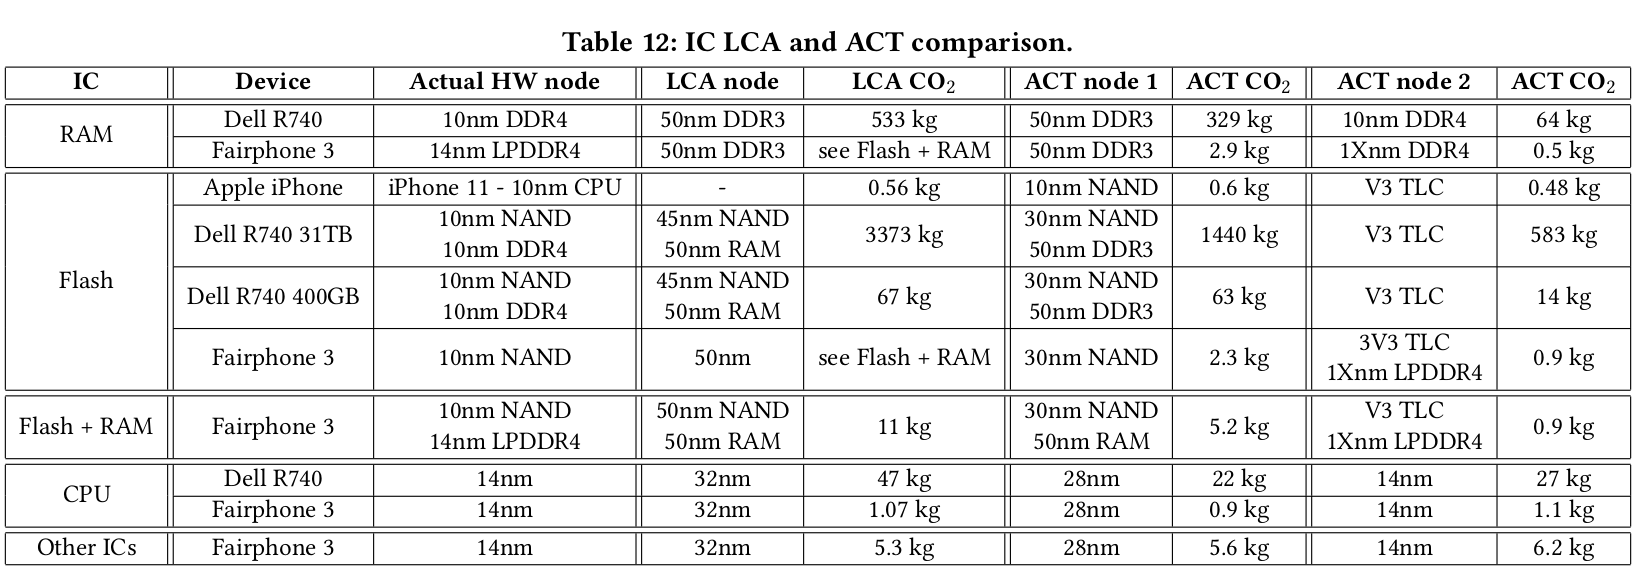
\includegraphics[width=.9\textwidth]{images/act_data.png}
      \caption{Impact of old data in LCA analysis\footfullcite{gupta2022_ACT}}
    \end{figure}    
  \end{center}  


\end{frame}



\end{document}

